\documentclass[twoside]{book}

% Packages required by doxygen
\usepackage{fixltx2e}
\usepackage{calc}
\usepackage{doxygen}
\usepackage[export]{adjustbox} % also loads graphicx
\usepackage{graphicx}
\usepackage[utf8]{inputenc}
\usepackage{makeidx}
\usepackage{multicol}
\usepackage{multirow}
\PassOptionsToPackage{warn}{textcomp}
\usepackage{textcomp}
\usepackage[nointegrals]{wasysym}
\usepackage[table]{xcolor}

% Font selection
\usepackage[T1]{fontenc}
\usepackage[scaled=.90]{helvet}
\usepackage{courier}
\usepackage{amssymb}
\usepackage{sectsty}
\renewcommand{\familydefault}{\sfdefault}
\allsectionsfont{%
  \fontseries{bc}\selectfont%
  \color{darkgray}%
}
\renewcommand{\DoxyLabelFont}{%
  \fontseries{bc}\selectfont%
  \color{darkgray}%
}
\newcommand{\+}{\discretionary{\mbox{\scriptsize$\hookleftarrow$}}{}{}}

% Page & text layout
\usepackage{geometry}
\geometry{%
  a4paper,%
  top=2.5cm,%
  bottom=2.5cm,%
  left=2.5cm,%
  right=2.5cm%
}
\tolerance=750
\hfuzz=15pt
\hbadness=750
\setlength{\emergencystretch}{15pt}
\setlength{\parindent}{0cm}
\setlength{\parskip}{3ex plus 2ex minus 2ex}
\makeatletter
\renewcommand{\paragraph}{%
  \@startsection{paragraph}{4}{0ex}{-1.0ex}{1.0ex}{%
    \normalfont\normalsize\bfseries\SS@parafont%
  }%
}
\renewcommand{\subparagraph}{%
  \@startsection{subparagraph}{5}{0ex}{-1.0ex}{1.0ex}{%
    \normalfont\normalsize\bfseries\SS@subparafont%
  }%
}
\makeatother

% Headers & footers
\usepackage{fancyhdr}
\pagestyle{fancyplain}
\fancyhead[LE]{\fancyplain{}{\bfseries\thepage}}
\fancyhead[CE]{\fancyplain{}{}}
\fancyhead[RE]{\fancyplain{}{\bfseries\leftmark}}
\fancyhead[LO]{\fancyplain{}{\bfseries\rightmark}}
\fancyhead[CO]{\fancyplain{}{}}
\fancyhead[RO]{\fancyplain{}{\bfseries\thepage}}
\fancyfoot[LE]{\fancyplain{}{}}
\fancyfoot[CE]{\fancyplain{}{}}
\fancyfoot[RE]{\fancyplain{}{\bfseries\scriptsize Generated by Doxygen }}
\fancyfoot[LO]{\fancyplain{}{\bfseries\scriptsize Generated by Doxygen }}
\fancyfoot[CO]{\fancyplain{}{}}
\fancyfoot[RO]{\fancyplain{}{}}
\renewcommand{\footrulewidth}{0.4pt}
\renewcommand{\chaptermark}[1]{%
  \markboth{#1}{}%
}
\renewcommand{\sectionmark}[1]{%
  \markright{\thesection\ #1}%
}

% Indices & bibliography
\usepackage{natbib}
\usepackage[titles]{tocloft}
\setcounter{tocdepth}{3}
\setcounter{secnumdepth}{5}
\makeindex

% Hyperlinks (required, but should be loaded last)
\usepackage{ifpdf}
\ifpdf
  \usepackage[pdftex,pagebackref=true]{hyperref}
\else
  \usepackage[ps2pdf,pagebackref=true]{hyperref}
\fi
\hypersetup{%
  colorlinks=true,%
  linkcolor=blue,%
  citecolor=blue,%
  unicode%
}

% Custom commands
\newcommand{\clearemptydoublepage}{%
  \newpage{\pagestyle{empty}\cleardoublepage}%
}

\usepackage{caption}
\captionsetup{labelsep=space,justification=centering,font={bf},singlelinecheck=off,skip=4pt,position=top}

%===== C O N T E N T S =====

\begin{document}

% Titlepage & ToC
\hypersetup{pageanchor=false,
             bookmarksnumbered=true,
             pdfencoding=unicode
            }
\pagenumbering{alph}
\begin{titlepage}
\vspace*{7cm}
\begin{center}%
{\Large P\+Buffer }\\
\vspace*{1cm}
{\large Generated by Doxygen 1.8.13}\\
\end{center}
\end{titlepage}
\clearemptydoublepage
\pagenumbering{roman}
\tableofcontents
\clearemptydoublepage
\pagenumbering{arabic}
\hypersetup{pageanchor=true}

%--- Begin generated contents ---
\chapter{Adding Data to the Buffer}
\label{md_adding_data_to_the_buffer}
\Hypertarget{md_adding_data_to_the_buffer}
\subsection*{Symbol meanings}

Priority is indicated with the letters h, m, and l, indicating, high, medium and low priorities. Note there can be up to 8 levels of priority in practice, but here we will only deal with three for clarity. The number following the letter indicates the number of elements of this priority in the buffer.

x indicates unused but available storage in the buffer.

\subsubsection*{Adding data to an empty buffer}

\paragraph*{Initially\+:}


\begin{DoxyCode}
x  ->  x  ->  x  ->  x  ->  ...
T*
\end{DoxyCode}


Since the data to be added will be the only data in the buffer it will naturally be the highest priority data on the buffer. In this case we can simply add the data at the element indicated by the tail pointer (T$\ast$) and set the relevant head pointer (Hl$\ast$ or Hm$\ast$ or Hh$\ast$). We also need to set the active flag for the relevant priority to indicate we have data of this priority in the buffer.

\subsubsection*{Adding l1 becomes\+:}


\begin{DoxyCode}
l1  ->  x  ->  x  ->  x  ->  ...
T*
Hl*
\end{DoxyCode}


\subsection*{Adding data of the lowest priority to a partially full buffer containing only low priority}

\subsubsection*{Initially\+:}


\begin{DoxyCode}
l1  ->  l2  ->  l3  ->  x  ->  ...
T*
                Hl      Hl*
\end{DoxyCode}


Since the buffer contains data in a high priority first, through lower priorities, to lower priority order, to add data of the lowest priority we can simply add the data at the buffer position indicated by the relevant head pointer H$\ast$ and advance the Head Hl. The relevant active flag is already set, but we set it anyway since it is quicker to just set the flag than test the flag and set it.

\subsubsection*{Adding l4 becomes\+:}


\begin{DoxyCode}
l1  ->  l2  ->  l3  ->  l4  ->  x  ...
T*
                        Hl      Hl*
\end{DoxyCode}


\subsection*{Adding data of the lowest priority to a partially full buffer containing mixed priorities}

\subsubsection*{Initially\+:}


\begin{DoxyCode}
h1  ->  h2  ->  h3  -> m1  ->  m2  ->  m3  ->  l1  ->  x  ->  ...
T*
                Hh                     Hm      Hl      Hl*
\end{DoxyCode}


Similarly to the previous example, here we simply add the new element to the buffer at the position indicated by the relevant head pointer. We then advance the relevant head and set the relevant active flag. Since the added data is of the lowest priority it needs to be at the end of the buffer, so we need to do anything more here.

\subsubsection*{Adding l2 becomes\+:}


\begin{DoxyCode}
h1  ->  h2  ->  h3  -> m1  ->  m2  ->  m3  ->  l1  ->  l2  ->  x  ->  ...
T*
                Hh                     Hm              Hl      Hl*
\end{DoxyCode}


\subsection*{Adding data of a high priority to a partially full buffer containing mixed priorities}

\subsubsection*{Initially\+:}


\begin{DoxyCode}
h1  ->  h2  ->  h3  -> m1  ->  m2  ->  m3  ->  l1  ->  x  ->  ...
T*
                Hh                     Hm      Hl      Hl*
\end{DoxyCode}


We now wish to add high priority data to a buffer of mixed priorities. In this case we need the data to be placed after data of a similar or higher priorities but before data of a lower priority. This is a two stage process. Stage 1 involves where to store the data in the physical buffer and stage 2 involves rearranging the buffer to set the data at the correct level of importance in the buffer, which is behind than data of a higher or similar priority, but ahead of lower priority data.

\subsubsection*{Adding h4 to the buffer\+:}

Since the buffer is not full we can add the data to an unused element (marked by x) that is pointed to by the lowest active Head pointer\+:

\subsubsection*{Stage 1\+:}


\begin{DoxyCode}
h1  ->  h2  ->  h3  -> m1  ->  m2  ->  m3  ->  l1  ->  h4  ->  x  ...
T*
                Hh                     Hm      Hl      Hl*
\end{DoxyCode}


The buffer is now out of order since we have higher priority data that is behind low priority data. We can correct this anomaly by remapping, or re-\/routing the buffer (since we have a link between adjacent elements). This is achieved by reassigning links in such a way that the new entry is placed behind data of higher and equal priority to itself, and ahead of data of lower priority to itself. This will re-\/establish the correct prioritisation in the buffer.

\subsubsection*{Finding the before insertion point\+:}

As indicated we need to place the data behind all data of higher or equal priority. To find this point we simply need to examine the activity flags starting at the current priority, and find the first active flag of equal or higher priority. If no such priority is active then we become the highest priority in the buffer and need to be inserted at the front of the buffer. If higher or equal priority exists we establish the priority closest to the current priority in increasing priority. In our case this is the highest priority. Therefore we need to be placed between the Hh head pointer and the element following. This is achieved by\+:


\begin{DoxyEnumerate}
\item saving the link at h3 in our case (which currently links to m1)
\item writing the position of the newly inserted data to the link at h3 (in our case the position of h4)
\item writing the current link of the newly inserted data to the pointer Hh$\ast$ link (in our case m1)
\item writing the saved link to the current link (in our case h4$\ast$)
\item setting the relevant head pointer to indicate the new priority head.
\item setting the relevant priority activity flag incase it hasn\textquotesingle{}t been set already.
\end{DoxyEnumerate}

\subsubsection*{Stage 2\+:}

Below shows how the links are broken and rearranged as above. The affect is to place the element h4 behind the element h3 and ahead of m1.


\begin{DoxyCode}
                    ------------------------------>
                      <------------------------------------
                                                    ------->
h1  ->  h2  ->  h3     m1  ->  m2  ->  m3  ->  l1      h4      x  ...
T*
\end{DoxyCode}
 Hm Hl Hh

Below we see the buffer after redrawing and allowing for re-\/linking\+:


\begin{DoxyCode}
h1  ->  h2  ->  h3  ->  h4  ->   m1  ->  m2  ->  m3  ->  l1  ->  x  ...
T*
                        Hh                       Hm      Hl
\end{DoxyCode}


\subsection*{Adding data to a full buffer}

To add data to a full buffer we are required to push the oldest lowest priority data \textquotesingle{}out the back\textquotesingle{} of the buffer, since we no longer have room to accomodate additional data. This ensures that the limited buffer space is reserved for the higher priority data and newer data of the lowest priority.

\subsection*{Attempting to add data of a lower priority that currently exists in a full buffer}

If the data to be added is of a lower priority than any of the data in the buffer (indicated by an inactive activity flag at the new priority), then the data is rejected, the buffer left untouched and an insertion error returned to the caller.

\subsection*{Adding data to a full buffer where the buffer is full of a single priority}

Where we are adding newer data to a full buffer containing only data of a similar priority we can simply overwrite the oldest data in the buffer with our newest data, and advance the tail pointer to the next position. In this way the latest insert is pushed to the back of the queue.

\subsubsection*{Initially\+:}


\begin{DoxyCode}
l1  ->  l2  ->  l3  ->  l4  ->   l5  ->  l6  ->  l7  ->  l8  ->  l9  ->  l10
T*                                                                       T
                                                                         Hl
\end{DoxyCode}


\subsubsection*{Adding l11 becomes\+:}


\begin{DoxyCode}
l11 ->  l2  ->  l3  ->  l4  ->   l5  ->  l6  ->  l7  ->  l8  ->  l9  ->  l10
T*                                                                       T
                                                                         Hl
\end{DoxyCode}
 \subsubsection*{Then advancing the Tail pointer\+:}


\begin{DoxyCode}
l2  ->  l3  ->  l4  ->   l5  ->  l6  ->  l7  ->  l8  ->  l9  ->  l10  ->  l11
T*                                                                        T
                                                                          Hl
\end{DoxyCode}


\subsection*{Adding data to a full buffer containing a mix of priority}

Assuming we have data of a higher or equal priority we can add it to the buffer by pushing less important data (older or lower priority) out of the buffer. This is a two stage process -\/ stage 1 is involved with determining where to store the new data -\/ stage 2 involves remapping or re-\/routing the links of the buffer to insert the data between data of higher importance (higher priority or newer) and data of lower importance (lower priority).

\subsubsection*{Stage 1\+:}

\paragraph*{To add m4\+:}


\begin{DoxyCode}
h1  ->  h2  ->  h3  ->  h4  ->   m1  ->  m2  ->  m3  ->  l1  ->  l2
T*                                                               T
                        Hh                       Hm              Hl
\end{DoxyCode}


Here we have a full buffer containing a mix of prioritisation. To add our data (m4) we need to determine the element containing the lowest priority and oldest element. In our case this is the element l1. Regardless of which priority we are adding this is the element to get overwritten since it it has the least importance.

\subsubsection*{Overwriting\+:}


\begin{DoxyCode}
h1  ->  h2  ->  h3  ->  h4  ->   m1  ->  m2  ->  m3  ->  m4  ->  l2
T*                                                               T
                        Hh                       Hm              Hl
\end{DoxyCode}


Here we need to overwrite l1 with m4 as shown. Since we haven\textquotesingle{}t a direct pointer to l1 we need to find l1 some other way. l1 can be considered the \textquotesingle{}tail\textquotesingle{} of priority \textquotesingle{}l\textquotesingle{}. This can be determined by finding the next highest priority on the buffer (that is the next active priority) and following the link of that priority\textquotesingle{}s relevant head. In our case the next highest priority to l1 is priority m. We follow the link given by the head Hm to l1 and overwrite m4 there.

In this case the buffer is still in the correct order and we simply need to advance the Hm head\+:


\begin{DoxyCode}
h1  ->  h2  ->  h3  ->  h4  ->   m1  ->  m2  ->  m3  ->  m4  ->  l2
T*                                                               T
                        Hh                               Hm      Hl
\end{DoxyCode}


\subsection*{Adding data to a full buffer of a priority higher than any on the buffer}

\subsubsection*{Initially\+:}


\begin{DoxyCode}
m1  ->  m2  ->  m3  ->  m4  ->  l1  ->  l2  ->  l3  ->  l4  ->   l5
T*                                                               T
                        Hm                                       Hl
\end{DoxyCode}


In this buffer we have data of priority m and data of priority l but no data of priority h. Say we need to add h1 to the buffer. We first need to identify the oldest, lowest priority element and overwrite it with the new data\+:

\subsubsection*{Overwriting l1 with h1\+:}


\begin{DoxyCode}
m1  ->  m2  ->  m3  ->  m4  ->  h1  ->  l2  ->  l3  ->  l4  ->   l5  (  ->  m1)
T*                                                               T   (      T*)
                        Hm                                       Hl
\end{DoxyCode}


Here we have overwritten l1 with h1. However the buffer clearly requires re-\/adjusting to correct the priorities. This is a similar process to that considered above.

\subsubsection*{Required adjustment\+:}


\begin{DoxyCode}
                             <------------------------------------
<------------------------------------
                            -------->
m1  ->  m2  ->  m3  ->  m4      h1      l2  ->  l3  ->  l4  ->   l5
T*                                                               T
                        Hm                                       Hl
\end{DoxyCode}


Notice here that the T$\ast$ needs to move since the higher priority becomes the front of the queue;

\subsubsection*{Rearranged gives\+:}


\begin{DoxyCode}
h1  ->  m1  ->  m2  ->  m3  ->  m4  ->  l2  ->  l3  ->  l4  ->   l5
T*                                                               T
                                Hm                               Hl
\end{DoxyCode}


\subsection*{Retrieving Data from the buffer\+:}

\subsubsection*{Initially\+:}


\begin{DoxyCode}
l1  ->  l2  ->  l3  ->  l4  ->   l5  ->  l6  ->  l7  ->  l8  ->  l9  ->  l10
T*                                                                       T
                                                                         Hl
\end{DoxyCode}


To remove data from the buffer we first check that the buffer is not empty. If it is empty an error is returned to the caller. If the buffer is not empty we return the element pointed to by the Tail pointer T$\ast$ and advance the Tail pointer.

\subsubsection*{Following retrieval\+:}


\begin{DoxyCode}
l2  ->  l3  ->  l4  ->   l5  ->  l6  ->  l7  ->  l8  ->  l9  ->  l10
T*                                                               T
                                                                 Hl
\end{DoxyCode}


We must determine whether we have depleted a particular priority from the buffer, and mark that priority inactive if this is the case. This is detected by comparing the highest active priority\textquotesingle{}s head pointer with the tail pointer prior to advancing the tail pointer. If they are equal we are about to deplete the highest priority and need to make the priority inactive\+:

\subsubsection*{Depleted Priority\+:}


\begin{DoxyCode}
h1  ->  l1  ->  l2  ->  l3  ->  l4  ->   l5  ->  l6  ->  l7  ->  l8
T*                                                               T
Hh                                                               Hl
\end{DoxyCode}


In this case there is only a single active priority on the buffer and a single relevant head pointer\+:

\subsubsection*{Becomes\+:}


\begin{DoxyCode}
l1  ->  l2  ->  l3  ->  l4  ->   l5  ->  l6  ->  l7  ->  l8
T*                                                       T
                                                         Hl
\end{DoxyCode}
 
\chapter{Theory of operation}
\label{md_src_theory_of_operation}
\Hypertarget{md_src_theory_of_operation}
This is a description of the theory of operation of this prioritorised circular buffer.

\subsection*{Configuration}

The buffer is configured at compile time by setting a small number of defines in priority\+\_\+buffer.\+h\+:

\#define B\+U\+F\+F\+E\+R\+\_\+\+S\+I\+ZE 4 /$\ast$ may be between 4 to 256 elements in size $\ast$/

\#define P\+R\+I\+O\+R\+I\+T\+Y\+\_\+\+S\+I\+ZE 3 /$\ast$ may be between 2 to 8 priorities in size $\ast$/

// \#define E\+L\+E\+M\+E\+N\+T\+\_\+\+S\+I\+ZE 8 /$\ast$ may be either 8, 16, 32, or 64 bits $\ast$/

The compiler checks these settings at compile time and compile will fail if they are out of limits.

These settings may also be provided on the command line to the compiler such as -\/\+D\+E\+L\+E\+M\+E\+N\+T\+\_\+\+S\+I\+ZE=8

priority\+\_\+buffer.\+h is purposefully kept very minimal to highlight these user configurations.

\subsection*{Design choice}

The design is optimised for smaller embedded devices, and should be suitable down to 8-\/bit devices.

\subsection*{Requirement Assumptions}

Due to the nature and size of the project it was decided to push through a design and then refactor for any wrong assumptions in the design and implementation. The design is unit-\/tested to ensure this refactoring is as painless as possible.

\subsection*{Memory}

The circular buffer is a structure containing elements upto the defined B\+U\+F\+F\+E\+R\+\_\+\+S\+I\+ZE. Each element is a structure containing both data and a forward-\/linking link to the following buffer location.

We also have a tail pointer and and array of head pointers whose size is equal to the P\+R\+I\+O\+R\+I\+T\+Y\+\_\+\+S\+I\+ZE. In addition, a further byte is used to store active flags for each priority.

With these pointers into the structure we can process both insert and retrieve operations very quickly. The only time we spend following the links to any extent (beyond one or two) is when we are requred to calculate the size of the buffer contents since it was decided the memory saved here was justifiable (the print function also follows the links, but this is a D\+E\+B\+UG enabled function only -\/ for the purpose of the command line evaluation program).

\subsection*{Pointers}

As mentioned, a number of pointers are used to provide fast access into the buffer\+:

1) Here P1 refers to highest priority, P3 to lowest priority etc. Tail is the tail pointer. Head is the head pointer. The active array maintains the active status. the x denotes an empty element.

-\/-\/-\/-\/-\/-\/-\/-\/-\/-\/-\/-\/-\/-\/-\/-\/-\/-\/---$<$-\/-\/-\/-\/-\/-\/-\/-\/-\/-\/-\/-\/-\/-\/-\/--- $\vert$ $\vert$ -\/$>$ P1 -\/$>$ P2 -\/$>$ P3 -\/$>$ x $>$-\/ $^\wedge$ $^\wedge$ $^\wedge$ $^\wedge$ Head\mbox{[}1\mbox{]} Head\mbox{[}2\mbox{]} Head\mbox{[}3\mbox{]} Tail

Active\mbox{[}1\mbox{]} = A\+C\+T\+I\+VE Active\mbox{[}2\mbox{]} = A\+C\+T\+I\+VE Active\mbox{[}3\mbox{]} = A\+C\+T\+I\+VE

\subsection*{Retrieving Data}

To retrieve an element the tail updates by following the link of the element it refernces, and the data at its new position is retrieved. If the head pointer matching the retrieved element\textquotesingle{}s priority has the same index value as the tail pointer, the relevant active flag is set to N\+O\+N\+\_\+\+A\+C\+T\+I\+VE.

If there is no data in the buffer all active flags are N\+O\+N\+\_\+\+A\+C\+T\+I\+VE and a suitable message returned to the caller. The empty buffer check is a single instruction operation.

\subsection*{Adding Data}

Since we prioritise the data added to the buffer the direction of priorities can be considered as flowing away from the tail from oldest high priority through newest high priority all the way down to oldest low priority through to newest low priority. This means that data is always retrieved highest priority first but in a first-\/ in-\/first-\/out manner considering the priority.

Elements are added to the buffer by the following means\+:

\subsubsection*{Buffer Empty}

If the buffer is empty, we add data to the location linked by the tail pointer. We ensure the data\textquotesingle{}s priority is noted on the relevant active flag, and assign the relevant priority head pointer with the array index of the element\textquotesingle{}s position in the buffer. In this way the priority head pointers always point to the newest element having that priority. If any active flag is I\+N\+A\+C\+T\+I\+VE the associated head pointer\textquotesingle{}s data is contains a meaningless value.

\subsubsection*{Buffer containing data but not full}

If the buffer is neither empty nor full, we add data to the location referenced by the `virtual master head\textquotesingle{} pointer. This is simply the index value of the lowest active priority pointer. In this case the data may be of a higher priority than its predecesser in which case we need to move it to the correct position. This is dealt with below by remapping the buffer.

\subsubsection*{Buffer Full}

If the buffer is full we need to determine if there is older data we can overwrite rather than throwing away this new data. This is achieved by the following strategy\+:

If there is data in the buffer having a priority that is either equal or of a lesser priority then we pick the lowest priority, and the oldest entry within that priority. We can reference this value by examining the priority head pointers and picking the next highest active priority to the one we want and following its link. This is where we need to overwrite our new data. It may happen that there is no higher priority active in which case our location is linked to by the value of the tail pointer index. Once we\textquotesingle{}ve overwritten the older data we will need to rearrange our links to relocate the latest entry to be at the end of it\textquotesingle{}s queue of identical priority. This is described below.

\subsection*{Remapping the buffer}

When data of varying priorities are added to the buffer we then need to rearrange the buffer to place the new element at the correct position in the buffer relevant to its priority. We are only concerned with remapping a single element since this is what we added, and the operation is very simple and quick. 
\chapter{Throw\+The\+Switch.\+org Coding Standard}
\label{md_test_unity_docs_ThrowTheSwitchCodingStandard}
\Hypertarget{md_test_unity_docs_ThrowTheSwitchCodingStandard}
Hi. Welcome to the coding standard for Throw\+The\+Switch.\+org. For the most part, we try to follow these standards to unify our contributors\textquotesingle{} code into a cohesive unit (puns intended). You might find places where these standards aren\textquotesingle{}t followed. We\textquotesingle{}re not perfect. Please be polite where you notice these discrepancies and we\textquotesingle{}ll try to be polite when we notice yours.

;)

\subsection*{Why Have A Coding Standard?}

Being consistent makes code easier to understand. We\textquotesingle{}ve tried to keep our standard simple because we also believe that we can only expect someone to follow something that is understandable. Please do your best.

\subsection*{Our Philosophy}

Before we get into details on syntax, let\textquotesingle{}s take a moment to talk about our vision for these tools. We\textquotesingle{}re C developers and embedded software developers. These tools are great to test any C code, but catering to embedded software has made us more tolerant of compiler quirks. There are a L\+OT of quirky compilers out there. By quirky I mean \char`\"{}doesn\textquotesingle{}t follow standards because they feel like
they have a license to do as they wish.\char`\"{}

Our philosophy is \char`\"{}support every compiler we can\char`\"{}. Most often, this means that we aim for writing C code that is standards compliant (often C89... that seems to be a sweet spot that is almost always compatible). But it also means these tools are tolerant of things that aren\textquotesingle{}t common. Some that aren\textquotesingle{}t even compliant. There are configuration options to override the size of standard types. There are configuration options to force Unity to not use certain standard library functions. A lot of Unity is configurable and we have worked hard to make it not T\+OO ugly in the process.

Similarly, our tools that parse C do their best. They aren\textquotesingle{}t full C parsers (yet) and, even if they were, they would still have to accept non-\/standard additions like gcc extensions or specifying {\ttfamily @0x1000} to force a variable to compile to a particular location. It\textquotesingle{}s just what we do, because we like everything to Just Work™.

Speaking of having things Just Work™, that\textquotesingle{}s our second philosophy. By that, we mean that we do our best to have E\+V\+E\+RY configuration option have a logical default. We believe that if you\textquotesingle{}re working with a simple compiler and target, you shouldn\textquotesingle{}t need to configure very much... we try to make the tools guess as much as they can, but give the user the power to override it when it\textquotesingle{}s wrong.

\subsection*{Naming Things}

Let\textquotesingle{}s talk about naming things. Programming is all about naming things. We name files, functions, variables, and so much more. While we\textquotesingle{}re not always going to find the best name for something, we actually put a bit of effort into finding $\ast$\+What Something W\+A\+N\+TS to be Called$\ast$™.

When naming things, we follow this hierarchy, the first being the most important to us (but we do all four when possible)\+:
\begin{DoxyEnumerate}
\item Readable
\item Descriptive
\item Consistent
\item Memorable
\end{DoxyEnumerate}

\paragraph*{Readable}

We want to read our code. This means we like names and flow that are more naturally read. We try to avoid double negatives. We try to avoid cryptic abbreviations (sticking to ones we feel are common).

\paragraph*{Descriptive}

We like descriptive names for things, especially functions and variables. Finding the right name for something is an important endeavor. You might notice from poking around our code that this often results in names that are a little longer than the average. Guilty. We\textquotesingle{}re okay with a bit more typing if it means our code is easier to understand.

There are two exceptions to this rule that we also stick to as religiously as possible\+:

First, while we realize hungarian notation (and similar systems for encoding type information into variable names) is providing a more descriptive name, we feel that (for the average developer) it takes away from readability and is to be avoided.

Second, loop counters and other local throw-\/away variables often have a purpose which is obvious. There\textquotesingle{}s no need, therefore, to get carried away with complex naming. We find i, j, and k are better loop counters than loop\+Counter\+Var or whatnot. We only break this rule when we see that more description could improve understanding of an algorithm.

\paragraph*{Consistent}

We like consistency, but we\textquotesingle{}re not really obsessed with it. We try to name our configuration macros in a consistent fashion... you\textquotesingle{}ll notice a repeated use of U\+N\+I\+T\+Y\+\_\+\+E\+X\+C\+L\+U\+D\+E\+\_\+\+B\+L\+AH or U\+N\+I\+T\+Y\+\_\+\+U\+S\+E\+S\+\_\+\+B\+L\+AH macros. This helps users avoid having to remember each macro\textquotesingle{}s details.

\paragraph*{Memorable}

Where ever it doesn\textquotesingle{}t violate the above principles, we try to apply memorable names. Sometimes this means using something that is simply descriptive, but often we strive for descriptive A\+ND unique... we like quirky names that stand out in our memory and are easier to search for. Take a look through the file names in Ceedling and you\textquotesingle{}ll get a good idea of what we are talking about here. Why use preprocess when you can use preprocessinator? Or what better describes a module in charge of invoking tasks during releases than release\+\_\+invoker? Don\textquotesingle{}t get carried away. The names are still descriptive and fulfill the above requirements, but they don\textquotesingle{}t feel stale.

\subsection*{C and C++ Details}

We don\textquotesingle{}t really want to add to the style battles out there. Tabs or spaces? How many spaces? Where do the braces go? These are age-\/old questions that will never be answered... or at least not answered in a way that will make everyone happy.

We\textquotesingle{}ve decided on our own style preferences. If you\textquotesingle{}d like to contribute to these projects (and we hope that you do), then we ask if you do your best to follow the same. It will only hurt a little. We promise.

\paragraph*{Whitespace}

Our C-\/style is to use spaces and to use 4 of them per indent level. It\textquotesingle{}s a nice power-\/of-\/2 number that looks decent on a wide-\/screen. We have no more reason than that. We break that rule when we have lines that wrap (macros or function arguments or whatnot). When that happens, we like to indent further to line things up in nice tidy columns.


\begin{DoxyCode}
\textcolor{keywordflow}{if} (stuff\_happened)
\{
    do\_something();
\}
\end{DoxyCode}


\paragraph*{Case}


\begin{DoxyItemize}
\item Files -\/ all lower case with underscores.
\item Variables -\/ all lower case with underscores
\item Macros -\/ all caps with underscores.
\item Typedefs -\/ all caps with underscores. (also ends with \+\_\+T).
\item Functions -\/ camel cased. Usually named Module\+Name\+\_\+\+Func\+Name
\item Constants and Globals -\/ camel cased.
\end{DoxyItemize}

\paragraph*{Braces}

The left brace is on the next line after the declaration. The right brace is directly below that. Everything in between in indented one level. If you\textquotesingle{}re catching an error and you have a one-\/line, go ahead and to it on the same line.


\begin{DoxyCode}
\textcolor{keywordflow}{while} (blah)
\{
    \textcolor{comment}{//Like so. Even if only one line, we use braces.}
\}
\end{DoxyCode}


\paragraph*{Comments}

Do you know what we hate? Old-\/school C block comments. B\+UT, we\textquotesingle{}re using them anyway. As we mentioned, our goal is to support every compiler we can, especially embedded compilers. There are S\+T\+I\+LL C compilers out there that only support old-\/school block comments. So that is what we\textquotesingle{}re using. We apologize. We think they are ugly too.

\subsection*{Ruby Details}

Is there really such thing as a Ruby coding standard? Ruby is such a free form language, it seems almost sacrilegious to suggest that people should comply to one method! We\textquotesingle{}ll keep it really brief!

\paragraph*{Whitespace}

Our Ruby style is to use spaces and to use 2 of them per indent level. It\textquotesingle{}s a nice power-\/of-\/2 number that really grooves with Ruby\textquotesingle{}s compact style. We have no more reason than that. We break that rule when we have lines that wrap. When that happens, we like to indent further to line things up in nice tidy columns.

\paragraph*{Case}


\begin{DoxyItemize}
\item Files -\/ all lower case with underscores.
\item Variables -\/ all lower case with underscores
\item Classes, Modules, etc -\/ Camel cased.
\item Functions -\/ all lower case with underscores
\item Constants -\/ all upper case with underscores
\end{DoxyItemize}

\subsection*{Documentation}

Egad. Really? We use mark down and we like pdf files because they can be made to look nice while still being portable. Good enough?

{\itshape Find The Latest of This And More at \href{https://throwtheswitch.org}{\tt Throw\+The\+Switch.\+org}} 
\chapter{Unity Assertions Reference}
\label{md_test_unity_docs_UnityAssertionsReference}
\Hypertarget{md_test_unity_docs_UnityAssertionsReference}
\subsection*{Background and Overview}

\subsubsection*{Super Condensed Version}


\begin{DoxyItemize}
\item An assertion establishes truth (i.\+e. boolean True) for a single condition. Upon boolean False, an assertion stops execution and reports the failure.
\item Unity is mainly a rich collection of assertions and the support to gather up and easily execute those assertions.
\item The structure of Unity allows you to easily separate test assertions from source code in, well, test code.
\item Unity\textquotesingle{}s assertions\+:
\item Come in many, many flavors to handle different C types and assertion cases.
\item Use context to provide detailed and helpful failure messages.
\item Document types, expected values, and basic behavior in your source code for free.
\end{DoxyItemize}

\subsubsection*{Unity Is Several Things But Mainly It\textquotesingle{}s Assertions}

One way to think of Unity is simply as a rich collection of assertions you can use to establish whether your source code behaves the way you think it does. Unity provides a framework to easily organize and execute those assertions in test code separate from your source code.

\subsubsection*{What\textquotesingle{}s an Assertion?}

At their core, assertions are an establishment of truth -\/ boolean truth. Was this thing equal to that thing? Does that code doohickey have such-\/and-\/such property or not? You get the idea. Assertions are executable code (to appreciate the big picture on this read up on the difference between \mbox{[}link\+:Dynamic Verification and Static Analysis\mbox{]}). A failing assertion stops execution and reports an error through some appropriate I/O channel (e.\+g. stdout, G\+UI, file, blinky light).

Fundamentally, for dynamic verification all you need is a single assertion mechanism. In fact, that\textquotesingle{}s what the \href{http://en.wikipedia.org/en/wiki/Assert.h}{\tt assert() macro in C\textquotesingle{}s standard library} is for. So why not just use it? Well, we can do far better in the reporting department. C\textquotesingle{}s {\ttfamily assert()} is pretty dumb as-\/is and is particularly poor for handling common data types like arrays, structs, etc. And, without some other support, it\textquotesingle{}s far too tempting to litter source code with C\textquotesingle{}s {\ttfamily assert()}\textquotesingle{}s. It\textquotesingle{}s generally much cleaner, manageable, and more useful to separate test and source code in the way Unity facilitates.

\subsubsection*{Unity\textquotesingle{}s Assertions\+: Helpful Messages {\itshape and} Free Source Code Documentation}

Asserting a simple truth condition is valuable, but using the context of the assertion is even more valuable. For instance, if you know you\textquotesingle{}re comparing bit flags and not just integers, then why not use that context to give explicit, readable, bit-\/level feedback when an assertion fails?

That\textquotesingle{}s what Unity\textquotesingle{}s collection of assertions do -\/ capture context to give you helpful, meaningful assertion failure messages. In fact, the assertions themselves also serve as executable documentation about types and values in your source code. So long as your tests remain current with your source and all those tests pass, you have a detailed, up-\/to-\/date view of the intent and mechanisms in your source code. And due to a wondrous mystery, well-\/tested code usually tends to be well designed code.

\subsection*{Assertion Conventions and Configurations}

\subsubsection*{Naming and Parameter Conventions}

The convention of assertion parameters generally follows this order\+: \begin{DoxyVerb}TEST_ASSERT_X( {modifiers}, {expected}, actual, {size/count} )
\end{DoxyVerb}


The very simplest assertion possible uses only a single \char`\"{}actual\char`\"{} parameter (e.\+g. a simple null check).

\char`\"{}\+Actual\char`\"{} is the value being tested and unlike the other parameters in an assertion construction is the only parameter present in all assertion variants. \char`\"{}\+Modifiers\char`\"{} are masks, ranges, bit flag specifiers, floating point deltas. \char`\"{}\+Expected\char`\"{} is your expected value (duh) to compare to an \char`\"{}actual\char`\"{} value; it\textquotesingle{}s marked as an optional parameter because some assertions only need a single \char`\"{}actual\char`\"{} parameter (e.\+g. null check). \char`\"{}\+Size/count\char`\"{} refers to string lengths, number of array elements, etc.

Many of Unity\textquotesingle{}s assertions are clear duplications in that the same data type is handled by several assertions. The differences among these are in how failure messages are presented. For instance, a {\ttfamily \+\_\+\+H\+EX} variant of an assertion prints the expected and actual values of that assertion formatted as hexadecimal.

\paragraph*{T\+E\+S\+T\+\_\+\+A\+S\+S\+E\+R\+T\+\_\+\+X\+\_\+\+M\+E\+S\+S\+A\+GE Variants}

{\itshape All} assertions are complemented with a variant that includes a simple string message as a final parameter. The string you specify is appended to an assertion failure message in Unity output.

For brevity, the assertion variants with a message parameter are not listed below. Just tack on {\ttfamily \+\_\+\+M\+E\+S\+S\+A\+GE} as the final component to any assertion name in the reference list below and add a string as the final parameter.

{\itshape Example\+:} \begin{DoxyVerb}TEST_ASSERT_X( {modifiers}, {expected}, actual, {size/count} )
\end{DoxyVerb}


becomes messageified like thus... \begin{DoxyVerb}TEST_ASSERT_X_MESSAGE( {modifiers}, {expected}, actual, {size/count}, message )
\end{DoxyVerb}


Notes\+:
\begin{DoxyItemize}
\item The {\ttfamily \+\_\+\+M\+E\+S\+S\+A\+GE} variants intentionally do not support {\ttfamily printf} style formatting since many embedded projects don\textquotesingle{}t support or avoid {\ttfamily printf} for various reasons. It is possible to use {\ttfamily sprintf} before the assertion to assemble a complex fail message, if necessary.
\item If you want to output a counter value within an assertion fail message (e.\+g. from a loop) , building up an array of results and then using one of the {\ttfamily \+\_\+\+A\+R\+R\+AY} assertions (see below) might be a handy alternative to {\ttfamily sprintf}.
\end{DoxyItemize}

\paragraph*{T\+E\+S\+T\+\_\+\+A\+S\+S\+E\+R\+T\+\_\+\+X\+\_\+\+A\+R\+R\+AY Variants}

Unity provides a collection of assertions for arrays containing a variety of types. These are documented in the Array section below. These are almost on par with the {\ttfamily \+\_\+\+M\+E\+S\+S\+A\+GE}variants of Unity\textquotesingle{}s Asserts in that for pretty much any Unity type assertion you can tack on {\ttfamily \+\_\+\+A\+R\+R\+AY} and run assertions on an entire block of memory. \begin{DoxyVerb}TEST_ASSERT_EQUAL_TYPEX_ARRAY( expected, actual, {size/count} )
\end{DoxyVerb}


\char`\"{}\+Expected\char`\"{} is an array itself. \char`\"{}\+Size/count\char`\"{} is one or two parameters necessary to establish the number of array elements and perhaps the length of elements within the array.

Notes\+:
\begin{DoxyItemize}
\item The {\ttfamily \+\_\+\+M\+E\+S\+S\+A\+GE} variant convention still applies here to array assertions. The {\ttfamily \+\_\+\+M\+E\+S\+S\+A\+GE} variants of the {\ttfamily \+\_\+\+A\+R\+R\+AY} assertions have names ending with {\ttfamily \+\_\+\+A\+R\+R\+A\+Y\+\_\+\+M\+E\+S\+S\+A\+GE}.
\item Assertions for handling arrays of floating point values are grouped with float and double assertions (see immediately following section).
\end{DoxyItemize}

\subsubsection*{T\+E\+S\+T\+\_\+\+A\+S\+S\+E\+R\+T\+\_\+\+E\+A\+C\+H\+\_\+\+E\+Q\+U\+A\+L\+\_\+X Variants}

Unity provides a collection of assertions for arrays containing a variety of types which can be compared to a single value as well. These are documented in the Each Equal section below. these are almost on par with the {\ttfamily \+\_\+\+M\+E\+S\+S\+A\+GE} variants of Unity\textquotesingle{}s Asserts in that for pretty much any Unity type assertion you can inject \+\_\+\+E\+A\+C\+H\+\_\+\+E\+Q\+U\+AL and run assertions on an entire block of memory. \begin{DoxyVerb}TEST_ASSERT_EACH_EQUAL_TYPEX( expected, actual, {size/count} )
\end{DoxyVerb}


\char`\"{}\+Expected\char`\"{} is a single value to compare to. \char`\"{}\+Actual\char`\"{} is an array where each element will be compared to the expected value. \char`\"{}\+Size/count\char`\"{} is one of two parameters necessary to establish the number of array elements and perhaps the length of elements within the array.

Notes\+:
\begin{DoxyItemize}
\item The {\ttfamily \+\_\+\+M\+E\+S\+S\+A\+GE} variant convention still applies here to Each Equal assertions.
\item Assertions for handling Each Equal of floating point values are grouped with float and double assertions (see immediately following section).
\end{DoxyItemize}

\subsubsection*{Configuration}

\paragraph*{Floating Point Support Is Optional}

Support for floating point types is configurable. That is, by defining the appropriate preprocessor symbols, floats and doubles can be individually enabled or disabled in Unity code. This is useful for embedded targets with no floating point math support (i.\+e. Unity compiles free of errors for fixed point only platforms). See Unity documentation for specifics.

\paragraph*{Maximum Data Type Width Is Configurable}

Not all targets support 64 bit wide types or even 32 bit wide types. Define the appropriate preprocessor symbols and Unity will omit all operations from compilation that exceed the maximum width of your target. See Unity documentation for specifics.

\subsection*{The Assertions in All Their Blessed Glory}

\subsubsection*{Basic Fail and Ignore}

\subparagraph*{{\ttfamily T\+E\+S\+T\+\_\+\+F\+A\+I\+L()}}

This fella is most often used in special conditions where your test code is performing logic beyond a simple assertion. That is, in practice, {\ttfamily T\+E\+S\+T\+\_\+\+F\+A\+I\+L()} will always be found inside a conditional code block.

{\itshape Examples\+:}
\begin{DoxyItemize}
\item Executing a state machine multiple times that increments a counter your test code then verifies as a final step.
\item Triggering an exception and verifying it (as in Try / Catch / Throw -\/ see the \href{https://github.com/ThrowTheSwitch/CException}{\tt C\+Exception} project).
\end{DoxyItemize}

\subparagraph*{{\ttfamily T\+E\+S\+T\+\_\+\+I\+G\+N\+O\+R\+E()}}

Marks a test case (i.\+e. function meant to contain test assertions) as ignored. Usually this is employed as a breadcrumb to come back and implement a test case. An ignored test case has effects if other assertions are in the enclosing test case (see Unity documentation for more).

\subsubsection*{Boolean}

\subparagraph*{{\ttfamily T\+E\+S\+T\+\_\+\+A\+S\+S\+E\+RT (condition)}}

\subparagraph*{{\ttfamily T\+E\+S\+T\+\_\+\+A\+S\+S\+E\+R\+T\+\_\+\+T\+R\+UE (condition)}}

\subparagraph*{{\ttfamily T\+E\+S\+T\+\_\+\+A\+S\+S\+E\+R\+T\+\_\+\+F\+A\+L\+SE (condition)}}

\subparagraph*{{\ttfamily T\+E\+S\+T\+\_\+\+A\+S\+S\+E\+R\+T\+\_\+\+U\+N\+L\+E\+SS (condition)}}

A simple wording variation on {\ttfamily T\+E\+S\+T\+\_\+\+A\+S\+S\+E\+R\+T\+\_\+\+F\+A\+L\+SE}.The semantics of {\ttfamily T\+E\+S\+T\+\_\+\+A\+S\+S\+E\+R\+T\+\_\+\+U\+N\+L\+E\+SS} aid readability in certain test constructions or conditional statements.

\subparagraph*{{\ttfamily T\+E\+S\+T\+\_\+\+A\+S\+S\+E\+R\+T\+\_\+\+N\+U\+LL (pointer)}}

\subparagraph*{{\ttfamily T\+E\+S\+T\+\_\+\+A\+S\+S\+E\+R\+T\+\_\+\+N\+O\+T\+\_\+\+N\+U\+LL (pointer)}}

\subsubsection*{Signed and Unsigned Integers (of all sizes)}

Large integer sizes can be disabled for build targets that do not support them. For example, if your target only supports up to 16 bit types, by defining the appropriate symbols Unity can be configured to omit 32 and 64 bit operations that would break compilation (see Unity documentation for more). Refer to Advanced Asserting later in this document for advice on dealing with other word sizes.

\subparagraph*{{\ttfamily T\+E\+S\+T\+\_\+\+A\+S\+S\+E\+R\+T\+\_\+\+E\+Q\+U\+A\+L\+\_\+\+I\+NT (expected, actual)}}

\subparagraph*{{\ttfamily T\+E\+S\+T\+\_\+\+A\+S\+S\+E\+R\+T\+\_\+\+E\+Q\+U\+A\+L\+\_\+\+I\+N\+T8 (expected, actual)}}

\subparagraph*{{\ttfamily T\+E\+S\+T\+\_\+\+A\+S\+S\+E\+R\+T\+\_\+\+E\+Q\+U\+A\+L\+\_\+\+I\+N\+T16 (expected, actual)}}

\subparagraph*{{\ttfamily T\+E\+S\+T\+\_\+\+A\+S\+S\+E\+R\+T\+\_\+\+E\+Q\+U\+A\+L\+\_\+\+I\+N\+T32 (expected, actual)}}

\subparagraph*{{\ttfamily T\+E\+S\+T\+\_\+\+A\+S\+S\+E\+R\+T\+\_\+\+E\+Q\+U\+A\+L\+\_\+\+I\+N\+T64 (expected, actual)}}

\subparagraph*{{\ttfamily T\+E\+S\+T\+\_\+\+A\+S\+S\+E\+R\+T\+\_\+\+E\+Q\+U\+AL (expected, actual)}}

\subparagraph*{{\ttfamily T\+E\+S\+T\+\_\+\+A\+S\+S\+E\+R\+T\+\_\+\+N\+O\+T\+\_\+\+E\+Q\+U\+AL (expected, actual)}}

\subparagraph*{{\ttfamily T\+E\+S\+T\+\_\+\+A\+S\+S\+E\+R\+T\+\_\+\+E\+Q\+U\+A\+L\+\_\+\+U\+I\+NT (expected, actual)}}

\subparagraph*{{\ttfamily T\+E\+S\+T\+\_\+\+A\+S\+S\+E\+R\+T\+\_\+\+E\+Q\+U\+A\+L\+\_\+\+U\+I\+N\+T8 (expected, actual)}}

\subparagraph*{{\ttfamily T\+E\+S\+T\+\_\+\+A\+S\+S\+E\+R\+T\+\_\+\+E\+Q\+U\+A\+L\+\_\+\+U\+I\+N\+T16 (expected, actual)}}

\subparagraph*{{\ttfamily T\+E\+S\+T\+\_\+\+A\+S\+S\+E\+R\+T\+\_\+\+E\+Q\+U\+A\+L\+\_\+\+U\+I\+N\+T32 (expected, actual)}}

\subparagraph*{{\ttfamily T\+E\+S\+T\+\_\+\+A\+S\+S\+E\+R\+T\+\_\+\+E\+Q\+U\+A\+L\+\_\+\+U\+I\+N\+T64 (expected, actual)}}

\subsubsection*{Unsigned Integers (of all sizes) in Hexadecimal}

All {\ttfamily \+\_\+\+H\+EX} assertions are identical in function to unsigned integer assertions but produce failure messages with the {\ttfamily expected} and {\ttfamily actual} values formatted in hexadecimal. Unity output is big endian.

\subparagraph*{{\ttfamily T\+E\+S\+T\+\_\+\+A\+S\+S\+E\+R\+T\+\_\+\+E\+Q\+U\+A\+L\+\_\+\+H\+EX (expected, actual)}}

\subparagraph*{{\ttfamily T\+E\+S\+T\+\_\+\+A\+S\+S\+E\+R\+T\+\_\+\+E\+Q\+U\+A\+L\+\_\+\+H\+E\+X8 (expected, actual)}}

\subparagraph*{{\ttfamily T\+E\+S\+T\+\_\+\+A\+S\+S\+E\+R\+T\+\_\+\+E\+Q\+U\+A\+L\+\_\+\+H\+E\+X16 (expected, actual)}}

\subparagraph*{{\ttfamily T\+E\+S\+T\+\_\+\+A\+S\+S\+E\+R\+T\+\_\+\+E\+Q\+U\+A\+L\+\_\+\+H\+E\+X32 (expected, actual)}}

\subparagraph*{{\ttfamily T\+E\+S\+T\+\_\+\+A\+S\+S\+E\+R\+T\+\_\+\+E\+Q\+U\+A\+L\+\_\+\+H\+E\+X64 (expected, actual)}}

\subsubsection*{Masked and Bit-\/level Assertions}

Masked and bit-\/level assertions produce output formatted in hexadecimal. Unity output is big endian.

\subparagraph*{{\ttfamily T\+E\+S\+T\+\_\+\+A\+S\+S\+E\+R\+T\+\_\+\+B\+I\+TS (mask, expected, actual)}}

Only compares the masked (i.\+e. high) bits of {\ttfamily expected} and {\ttfamily actual} parameters.

\subparagraph*{{\ttfamily T\+E\+S\+T\+\_\+\+A\+S\+S\+E\+R\+T\+\_\+\+B\+I\+T\+S\+\_\+\+H\+I\+GH (mask, actual)}}

Asserts the masked bits of the {\ttfamily actual} parameter are high.

\subparagraph*{{\ttfamily T\+E\+S\+T\+\_\+\+A\+S\+S\+E\+R\+T\+\_\+\+B\+I\+T\+S\+\_\+\+L\+OW (mask, actual)}}

Asserts the masked bits of the {\ttfamily actual} parameter are low.

\subparagraph*{{\ttfamily T\+E\+S\+T\+\_\+\+A\+S\+S\+E\+R\+T\+\_\+\+B\+I\+T\+\_\+\+H\+I\+GH (bit, actual)}}

Asserts the specified bit of the {\ttfamily actual} parameter is high.

\subparagraph*{{\ttfamily T\+E\+S\+T\+\_\+\+A\+S\+S\+E\+R\+T\+\_\+\+B\+I\+T\+\_\+\+L\+OW (bit, actual)}}

Asserts the specified bit of the {\ttfamily actual} parameter is low.

\subsubsection*{Integer Less Than / Greater Than}

These assertions verify that the {\ttfamily actual} parameter is less than or greater than {\ttfamily threshold} (exclusive). For example, if the threshold value is 0 for the greater than assertion will fail if it is 0 or less.

\subparagraph*{{\ttfamily T\+E\+S\+T\+\_\+\+A\+S\+S\+E\+R\+T\+\_\+\+G\+R\+E\+A\+T\+E\+R\+\_\+\+T\+H\+AN (threshold, actual)}}

\subparagraph*{{\ttfamily T\+E\+S\+T\+\_\+\+A\+S\+S\+E\+R\+T\+\_\+\+G\+R\+E\+A\+T\+E\+R\+\_\+\+T\+H\+A\+N\+\_\+\+I\+NT (threshold, actual)}}

\subparagraph*{{\ttfamily T\+E\+S\+T\+\_\+\+A\+S\+S\+E\+R\+T\+\_\+\+G\+R\+E\+A\+T\+E\+R\+\_\+\+T\+H\+A\+N\+\_\+\+I\+N\+T8 (threshold, actual)}}

\subparagraph*{{\ttfamily T\+E\+S\+T\+\_\+\+A\+S\+S\+E\+R\+T\+\_\+\+G\+R\+E\+A\+T\+E\+R\+\_\+\+T\+H\+A\+N\+\_\+\+I\+N\+T16 (threshold, actual)}}

\subparagraph*{{\ttfamily T\+E\+S\+T\+\_\+\+A\+S\+S\+E\+R\+T\+\_\+\+G\+R\+E\+A\+T\+E\+R\+\_\+\+T\+H\+A\+N\+\_\+\+I\+N\+T32 (threshold, actual)}}

\subparagraph*{{\ttfamily T\+E\+S\+T\+\_\+\+A\+S\+S\+E\+R\+T\+\_\+\+G\+R\+E\+A\+T\+E\+R\+\_\+\+T\+H\+A\+N\+\_\+\+U\+I\+NT (threshold, actual)}}

\subparagraph*{{\ttfamily T\+E\+S\+T\+\_\+\+A\+S\+S\+E\+R\+T\+\_\+\+G\+R\+E\+A\+T\+E\+R\+\_\+\+T\+H\+A\+N\+\_\+\+U\+I\+N\+T8 (threshold, actual)}}

\subparagraph*{{\ttfamily T\+E\+S\+T\+\_\+\+A\+S\+S\+E\+R\+T\+\_\+\+G\+R\+E\+A\+T\+E\+R\+\_\+\+T\+H\+A\+N\+\_\+\+U\+I\+N\+T16 (threshold, actual)}}

\subparagraph*{{\ttfamily T\+E\+S\+T\+\_\+\+A\+S\+S\+E\+R\+T\+\_\+\+G\+R\+E\+A\+T\+E\+R\+\_\+\+T\+H\+A\+N\+\_\+\+U\+I\+N\+T32 (threshold, actual)}}

\subparagraph*{{\ttfamily T\+E\+S\+T\+\_\+\+A\+S\+S\+E\+R\+T\+\_\+\+G\+R\+E\+A\+T\+E\+R\+\_\+\+T\+H\+A\+N\+\_\+\+H\+E\+X8 (threshold, actual)}}

\subparagraph*{{\ttfamily T\+E\+S\+T\+\_\+\+A\+S\+S\+E\+R\+T\+\_\+\+G\+R\+E\+A\+T\+E\+R\+\_\+\+T\+H\+A\+N\+\_\+\+H\+E\+X16 (threshold, actual)}}

\subparagraph*{{\ttfamily T\+E\+S\+T\+\_\+\+A\+S\+S\+E\+R\+T\+\_\+\+G\+R\+E\+A\+T\+E\+R\+\_\+\+T\+H\+A\+N\+\_\+\+H\+E\+X32 (threshold, actual)}}

\subparagraph*{{\ttfamily T\+E\+S\+T\+\_\+\+A\+S\+S\+E\+R\+T\+\_\+\+L\+E\+S\+S\+\_\+\+T\+H\+AN (threshold, actual)}}

\subparagraph*{{\ttfamily T\+E\+S\+T\+\_\+\+A\+S\+S\+E\+R\+T\+\_\+\+L\+E\+S\+S\+\_\+\+T\+H\+A\+N\+\_\+\+I\+NT (threshold, actual)}}

\subparagraph*{{\ttfamily T\+E\+S\+T\+\_\+\+A\+S\+S\+E\+R\+T\+\_\+\+L\+E\+S\+S\+\_\+\+T\+H\+A\+N\+\_\+\+I\+N\+T8 (threshold, actual)}}

\subparagraph*{{\ttfamily T\+E\+S\+T\+\_\+\+A\+S\+S\+E\+R\+T\+\_\+\+L\+E\+S\+S\+\_\+\+T\+H\+A\+N\+\_\+\+I\+N\+T16 (threshold, actual)}}

\subparagraph*{{\ttfamily T\+E\+S\+T\+\_\+\+A\+S\+S\+E\+R\+T\+\_\+\+L\+E\+S\+S\+\_\+\+T\+H\+A\+N\+\_\+\+I\+N\+T32 (threshold, actual)}}

\subparagraph*{{\ttfamily T\+E\+S\+T\+\_\+\+A\+S\+S\+E\+R\+T\+\_\+\+L\+E\+S\+S\+\_\+\+T\+H\+A\+N\+\_\+\+U\+I\+NT (threshold, actual)}}

\subparagraph*{{\ttfamily T\+E\+S\+T\+\_\+\+A\+S\+S\+E\+R\+T\+\_\+\+L\+E\+S\+S\+\_\+\+T\+H\+A\+N\+\_\+\+U\+I\+N\+T8 (threshold, actual)}}

\subparagraph*{{\ttfamily T\+E\+S\+T\+\_\+\+A\+S\+S\+E\+R\+T\+\_\+\+L\+E\+S\+S\+\_\+\+T\+H\+A\+N\+\_\+\+U\+I\+N\+T16 (threshold, actual)}}

\subparagraph*{{\ttfamily T\+E\+S\+T\+\_\+\+A\+S\+S\+E\+R\+T\+\_\+\+L\+E\+S\+S\+\_\+\+T\+H\+A\+N\+\_\+\+U\+I\+N\+T32 (threshold, actual)}}

\subparagraph*{{\ttfamily T\+E\+S\+T\+\_\+\+A\+S\+S\+E\+R\+T\+\_\+\+L\+E\+S\+S\+\_\+\+T\+H\+A\+N\+\_\+\+H\+E\+X8 (threshold, actual)}}

\subparagraph*{{\ttfamily T\+E\+S\+T\+\_\+\+A\+S\+S\+E\+R\+T\+\_\+\+L\+E\+S\+S\+\_\+\+T\+H\+A\+N\+\_\+\+H\+E\+X16 (threshold, actual)}}

\subparagraph*{{\ttfamily T\+E\+S\+T\+\_\+\+A\+S\+S\+E\+R\+T\+\_\+\+L\+E\+S\+S\+\_\+\+T\+H\+A\+N\+\_\+\+H\+E\+X32 (threshold, actual)}}

\subsubsection*{Integer Ranges (of all sizes)}

These assertions verify that the {\ttfamily expected} parameter is within +/-\/ {\ttfamily delta} (inclusive) of the {\ttfamily actual} parameter. For example, if the expected value is 10 and the delta is 3 then the assertion will fail for any value outside the range of 7 -\/ 13.

\subparagraph*{{\ttfamily T\+E\+S\+T\+\_\+\+A\+S\+S\+E\+R\+T\+\_\+\+I\+N\+T\+\_\+\+W\+I\+T\+H\+IN (delta, expected, actual)}}

\subparagraph*{{\ttfamily T\+E\+S\+T\+\_\+\+A\+S\+S\+E\+R\+T\+\_\+\+I\+N\+T8\+\_\+\+W\+I\+T\+H\+IN (delta, expected, actual)}}

\subparagraph*{{\ttfamily T\+E\+S\+T\+\_\+\+A\+S\+S\+E\+R\+T\+\_\+\+I\+N\+T16\+\_\+\+W\+I\+T\+H\+IN (delta, expected, actual)}}

\subparagraph*{{\ttfamily T\+E\+S\+T\+\_\+\+A\+S\+S\+E\+R\+T\+\_\+\+I\+N\+T32\+\_\+\+W\+I\+T\+H\+IN (delta, expected, actual)}}

\subparagraph*{{\ttfamily T\+E\+S\+T\+\_\+\+A\+S\+S\+E\+R\+T\+\_\+\+I\+N\+T64\+\_\+\+W\+I\+T\+H\+IN (delta, expected, actual)}}

\subparagraph*{{\ttfamily T\+E\+S\+T\+\_\+\+A\+S\+S\+E\+R\+T\+\_\+\+U\+I\+N\+T\+\_\+\+W\+I\+T\+H\+IN (delta, expected, actual)}}

\subparagraph*{{\ttfamily T\+E\+S\+T\+\_\+\+A\+S\+S\+E\+R\+T\+\_\+\+U\+I\+N\+T8\+\_\+\+W\+I\+T\+H\+IN (delta, expected, actual)}}

\subparagraph*{{\ttfamily T\+E\+S\+T\+\_\+\+A\+S\+S\+E\+R\+T\+\_\+\+U\+I\+N\+T16\+\_\+\+W\+I\+T\+H\+IN (delta, expected, actual)}}

\subparagraph*{{\ttfamily T\+E\+S\+T\+\_\+\+A\+S\+S\+E\+R\+T\+\_\+\+U\+I\+N\+T32\+\_\+\+W\+I\+T\+H\+IN (delta, expected, actual)}}

\subparagraph*{{\ttfamily T\+E\+S\+T\+\_\+\+A\+S\+S\+E\+R\+T\+\_\+\+U\+I\+N\+T64\+\_\+\+W\+I\+T\+H\+IN (delta, expected, actual)}}

\subparagraph*{{\ttfamily T\+E\+S\+T\+\_\+\+A\+S\+S\+E\+R\+T\+\_\+\+H\+E\+X\+\_\+\+W\+I\+T\+H\+IN (delta, expected, actual)}}

\subparagraph*{{\ttfamily T\+E\+S\+T\+\_\+\+A\+S\+S\+E\+R\+T\+\_\+\+H\+E\+X8\+\_\+\+W\+I\+T\+H\+IN (delta, expected, actual)}}

\subparagraph*{{\ttfamily T\+E\+S\+T\+\_\+\+A\+S\+S\+E\+R\+T\+\_\+\+H\+E\+X16\+\_\+\+W\+I\+T\+H\+IN (delta, expected, actual)}}

\subparagraph*{{\ttfamily T\+E\+S\+T\+\_\+\+A\+S\+S\+E\+R\+T\+\_\+\+H\+E\+X32\+\_\+\+W\+I\+T\+H\+IN (delta, expected, actual)}}

\subparagraph*{{\ttfamily T\+E\+S\+T\+\_\+\+A\+S\+S\+E\+R\+T\+\_\+\+H\+E\+X64\+\_\+\+W\+I\+T\+H\+IN (delta, expected, actual)}}

\subsubsection*{Structs and Strings}

\subparagraph*{{\ttfamily T\+E\+S\+T\+\_\+\+A\+S\+S\+E\+R\+T\+\_\+\+E\+Q\+U\+A\+L\+\_\+\+P\+TR (expected, actual)}}

Asserts that the pointers point to the same memory location.

\subparagraph*{{\ttfamily T\+E\+S\+T\+\_\+\+A\+S\+S\+E\+R\+T\+\_\+\+E\+Q\+U\+A\+L\+\_\+\+S\+T\+R\+I\+NG (expected, actual)}}

Asserts that the null terminated (`\textquotesingle{}\textbackslash{}0\textquotesingle{}`)strings are identical. If strings are of different lengths or any portion of the strings before their terminators differ, the assertion fails. Two N\+U\+LL strings (i.\+e. zero length) are considered equivalent.

\subparagraph*{{\ttfamily T\+E\+S\+T\+\_\+\+A\+S\+S\+E\+R\+T\+\_\+\+E\+Q\+U\+A\+L\+\_\+\+M\+E\+M\+O\+RY (expected, actual, len)}}

Asserts that the contents of the memory specified by the {\ttfamily expected} and {\ttfamily actual} pointers is identical. The size of the memory blocks in bytes is specified by the {\ttfamily len} parameter.

\subsubsection*{Arrays}

{\ttfamily expected} and {\ttfamily actual} parameters are both arrays. {\ttfamily num\+\_\+elements} specifies the number of elements in the arrays to compare.

{\ttfamily \+\_\+\+H\+EX} assertions produce failure messages with expected and actual array contents formatted in hexadecimal.

For array of strings comparison behavior, see comments for {\ttfamily T\+E\+S\+T\+\_\+\+A\+S\+S\+E\+R\+T\+\_\+\+E\+Q\+U\+A\+L\+\_\+\+S\+T\+R\+I\+NG} in the preceding section.

Assertions fail upon the first element in the compared arrays found not to match. Failure messages specify the array index of the failed comparison.

\subparagraph*{{\ttfamily T\+E\+S\+T\+\_\+\+A\+S\+S\+E\+R\+T\+\_\+\+E\+Q\+U\+A\+L\+\_\+\+I\+N\+T\+\_\+\+A\+R\+R\+AY (expected, actual, num\+\_\+elements)}}

\subparagraph*{{\ttfamily T\+E\+S\+T\+\_\+\+A\+S\+S\+E\+R\+T\+\_\+\+E\+Q\+U\+A\+L\+\_\+\+I\+N\+T8\+\_\+\+A\+R\+R\+AY (expected, actual, num\+\_\+elements)}}

\subparagraph*{{\ttfamily T\+E\+S\+T\+\_\+\+A\+S\+S\+E\+R\+T\+\_\+\+E\+Q\+U\+A\+L\+\_\+\+I\+N\+T16\+\_\+\+A\+R\+R\+AY (expected, actual, num\+\_\+elements)}}

\subparagraph*{{\ttfamily T\+E\+S\+T\+\_\+\+A\+S\+S\+E\+R\+T\+\_\+\+E\+Q\+U\+A\+L\+\_\+\+I\+N\+T32\+\_\+\+A\+R\+R\+AY (expected, actual, num\+\_\+elements)}}

\subparagraph*{{\ttfamily T\+E\+S\+T\+\_\+\+A\+S\+S\+E\+R\+T\+\_\+\+E\+Q\+U\+A\+L\+\_\+\+I\+N\+T64\+\_\+\+A\+R\+R\+AY (expected, actual, num\+\_\+elements)}}

\subparagraph*{{\ttfamily T\+E\+S\+T\+\_\+\+A\+S\+S\+E\+R\+T\+\_\+\+E\+Q\+U\+A\+L\+\_\+\+U\+I\+N\+T\+\_\+\+A\+R\+R\+AY (expected, actual, num\+\_\+elements)}}

\subparagraph*{{\ttfamily T\+E\+S\+T\+\_\+\+A\+S\+S\+E\+R\+T\+\_\+\+E\+Q\+U\+A\+L\+\_\+\+U\+I\+N\+T8\+\_\+\+A\+R\+R\+AY (expected, actual, num\+\_\+elements)}}

\subparagraph*{{\ttfamily T\+E\+S\+T\+\_\+\+A\+S\+S\+E\+R\+T\+\_\+\+E\+Q\+U\+A\+L\+\_\+\+U\+I\+N\+T16\+\_\+\+A\+R\+R\+AY (expected, actual, num\+\_\+elements)}}

\subparagraph*{{\ttfamily T\+E\+S\+T\+\_\+\+A\+S\+S\+E\+R\+T\+\_\+\+E\+Q\+U\+A\+L\+\_\+\+U\+I\+N\+T32\+\_\+\+A\+R\+R\+AY (expected, actual, num\+\_\+elements)}}

\subparagraph*{{\ttfamily T\+E\+S\+T\+\_\+\+A\+S\+S\+E\+R\+T\+\_\+\+E\+Q\+U\+A\+L\+\_\+\+U\+I\+N\+T64\+\_\+\+A\+R\+R\+AY (expected, actual, num\+\_\+elements)}}

\subparagraph*{{\ttfamily T\+E\+S\+T\+\_\+\+A\+S\+S\+E\+R\+T\+\_\+\+E\+Q\+U\+A\+L\+\_\+\+H\+E\+X\+\_\+\+A\+R\+R\+AY (expected, actual, num\+\_\+elements)}}

\subparagraph*{{\ttfamily T\+E\+S\+T\+\_\+\+A\+S\+S\+E\+R\+T\+\_\+\+E\+Q\+U\+A\+L\+\_\+\+H\+E\+X8\+\_\+\+A\+R\+R\+AY (expected, actual, num\+\_\+elements)}}

\subparagraph*{{\ttfamily T\+E\+S\+T\+\_\+\+A\+S\+S\+E\+R\+T\+\_\+\+E\+Q\+U\+A\+L\+\_\+\+H\+E\+X16\+\_\+\+A\+R\+R\+AY (expected, actual, num\+\_\+elements)}}

\subparagraph*{{\ttfamily T\+E\+S\+T\+\_\+\+A\+S\+S\+E\+R\+T\+\_\+\+E\+Q\+U\+A\+L\+\_\+\+H\+E\+X32\+\_\+\+A\+R\+R\+AY (expected, actual, num\+\_\+elements)}}

\subparagraph*{{\ttfamily T\+E\+S\+T\+\_\+\+A\+S\+S\+E\+R\+T\+\_\+\+E\+Q\+U\+A\+L\+\_\+\+H\+E\+X64\+\_\+\+A\+R\+R\+AY (expected, actual, num\+\_\+elements)}}

\subparagraph*{{\ttfamily T\+E\+S\+T\+\_\+\+A\+S\+S\+E\+R\+T\+\_\+\+E\+Q\+U\+A\+L\+\_\+\+P\+T\+R\+\_\+\+A\+R\+R\+AY (expected, actual, num\+\_\+elements)}}

\subparagraph*{{\ttfamily T\+E\+S\+T\+\_\+\+A\+S\+S\+E\+R\+T\+\_\+\+E\+Q\+U\+A\+L\+\_\+\+S\+T\+R\+I\+N\+G\+\_\+\+A\+R\+R\+AY (expected, actual, num\+\_\+elements)}}

\subparagraph*{{\ttfamily T\+E\+S\+T\+\_\+\+A\+S\+S\+E\+R\+T\+\_\+\+E\+Q\+U\+A\+L\+\_\+\+M\+E\+M\+O\+R\+Y\+\_\+\+A\+R\+R\+AY (expected, actual, len, num\+\_\+elements)}}

{\ttfamily len} is the memory in bytes to be compared at each array element.

\subsubsection*{Each Equal (Arrays to Single Value)}

{\ttfamily expected} are single values and {\ttfamily actual} are arrays. {\ttfamily num\+\_\+elements} specifies the number of elements in the arrays to compare.

{\ttfamily \+\_\+\+H\+EX} assertions produce failure messages with expected and actual array contents formatted in hexadecimal.

Assertions fail upon the first element in the compared arrays found not to match. Failure messages specify the array index of the failed comparison.

\paragraph*{{\ttfamily T\+E\+S\+T\+\_\+\+A\+S\+S\+E\+R\+T\+\_\+\+E\+A\+C\+H\+\_\+\+E\+Q\+U\+A\+L\+\_\+\+I\+NT (expected, actual, num\+\_\+elements)}}

\paragraph*{{\ttfamily T\+E\+S\+T\+\_\+\+A\+S\+S\+E\+R\+T\+\_\+\+E\+A\+C\+H\+\_\+\+E\+Q\+U\+A\+L\+\_\+\+I\+N\+T8 (expected, actual, num\+\_\+elements)}}

\paragraph*{{\ttfamily T\+E\+S\+T\+\_\+\+A\+S\+S\+E\+R\+T\+\_\+\+E\+A\+C\+H\+\_\+\+E\+Q\+U\+A\+L\+\_\+\+I\+N\+T16 (expected, actual, num\+\_\+elements)}}

\paragraph*{{\ttfamily T\+E\+S\+T\+\_\+\+A\+S\+S\+E\+R\+T\+\_\+\+E\+A\+C\+H\+\_\+\+E\+Q\+U\+A\+L\+\_\+\+I\+N\+T32 (expected, actual, num\+\_\+elements)}}

\paragraph*{{\ttfamily T\+E\+S\+T\+\_\+\+A\+S\+S\+E\+R\+T\+\_\+\+E\+A\+C\+H\+\_\+\+E\+Q\+U\+A\+L\+\_\+\+I\+N\+T64 (expected, actual, num\+\_\+elements)}}

\paragraph*{{\ttfamily T\+E\+S\+T\+\_\+\+A\+S\+S\+E\+R\+T\+\_\+\+E\+A\+C\+H\+\_\+\+E\+Q\+U\+A\+L\+\_\+\+U\+I\+NT (expected, actual, num\+\_\+elements)}}

\paragraph*{{\ttfamily T\+E\+S\+T\+\_\+\+A\+S\+S\+E\+R\+T\+\_\+\+E\+A\+C\+H\+\_\+\+E\+Q\+U\+A\+L\+\_\+\+U\+I\+N\+T8 (expected, actual, num\+\_\+elements)}}

\paragraph*{{\ttfamily T\+E\+S\+T\+\_\+\+A\+S\+S\+E\+R\+T\+\_\+\+E\+A\+C\+H\+\_\+\+E\+Q\+U\+A\+L\+\_\+\+U\+I\+N\+T16 (expected, actual, num\+\_\+elements)}}

\paragraph*{{\ttfamily T\+E\+S\+T\+\_\+\+A\+S\+S\+E\+R\+T\+\_\+\+E\+A\+C\+H\+\_\+\+E\+Q\+U\+A\+L\+\_\+\+U\+I\+N\+T32 (expected, actual, num\+\_\+elements)}}

\paragraph*{{\ttfamily T\+E\+S\+T\+\_\+\+A\+S\+S\+E\+R\+T\+\_\+\+E\+A\+C\+H\+\_\+\+E\+Q\+U\+A\+L\+\_\+\+U\+I\+N\+T64 (expected, actual, num\+\_\+elements)}}

\paragraph*{{\ttfamily T\+E\+S\+T\+\_\+\+A\+S\+S\+E\+R\+T\+\_\+\+E\+A\+C\+H\+\_\+\+E\+Q\+U\+A\+L\+\_\+\+H\+EX (expected, actual, num\+\_\+elements)}}

\paragraph*{{\ttfamily T\+E\+S\+T\+\_\+\+A\+S\+S\+E\+R\+T\+\_\+\+E\+A\+C\+H\+\_\+\+E\+Q\+U\+A\+L\+\_\+\+H\+E\+X8 (expected, actual, num\+\_\+elements)}}

\paragraph*{{\ttfamily T\+E\+S\+T\+\_\+\+A\+S\+S\+E\+R\+T\+\_\+\+E\+A\+C\+H\+\_\+\+E\+Q\+U\+A\+L\+\_\+\+H\+E\+X16 (expected, actual, num\+\_\+elements)}}

\paragraph*{{\ttfamily T\+E\+S\+T\+\_\+\+A\+S\+S\+E\+R\+T\+\_\+\+E\+A\+C\+H\+\_\+\+E\+Q\+U\+A\+L\+\_\+\+H\+E\+X32 (expected, actual, num\+\_\+elements)}}

\paragraph*{{\ttfamily T\+E\+S\+T\+\_\+\+A\+S\+S\+E\+R\+T\+\_\+\+E\+A\+C\+H\+\_\+\+E\+Q\+U\+A\+L\+\_\+\+H\+E\+X64 (expected, actual, num\+\_\+elements)}}

\paragraph*{{\ttfamily T\+E\+S\+T\+\_\+\+A\+S\+S\+E\+R\+T\+\_\+\+E\+A\+C\+H\+\_\+\+E\+Q\+U\+A\+L\+\_\+\+P\+TR (expected, actual, num\+\_\+elements)}}

\paragraph*{{\ttfamily T\+E\+S\+T\+\_\+\+A\+S\+S\+E\+R\+T\+\_\+\+E\+A\+C\+H\+\_\+\+E\+Q\+U\+A\+L\+\_\+\+S\+T\+R\+I\+NG (expected, actual, num\+\_\+elements)}}

\paragraph*{{\ttfamily T\+E\+S\+T\+\_\+\+A\+S\+S\+E\+R\+T\+\_\+\+E\+A\+C\+H\+\_\+\+E\+Q\+U\+A\+L\+\_\+\+M\+E\+M\+O\+RY (expected, actual, len, num\+\_\+elements)}}

{\ttfamily len} is the memory in bytes to be compared at each array element.

\subsubsection*{Floating Point (If enabled)}

\subparagraph*{{\ttfamily T\+E\+S\+T\+\_\+\+A\+S\+S\+E\+R\+T\+\_\+\+F\+L\+O\+A\+T\+\_\+\+W\+I\+T\+H\+IN (delta, expected, actual)}}

Asserts that the {\ttfamily actual} value is within +/-\/ {\ttfamily delta} of the {\ttfamily expected} value. The nature of floating point representation is such that exact evaluations of equality are not guaranteed.

\subparagraph*{{\ttfamily T\+E\+S\+T\+\_\+\+A\+S\+S\+E\+R\+T\+\_\+\+E\+Q\+U\+A\+L\+\_\+\+F\+L\+O\+AT (expected, actual)}}

Asserts that the ?actual?value is \char`\"{}close enough to be considered equal\char`\"{} to the {\ttfamily expected} value. If you are curious about the details, refer to the Advanced Asserting section for more details on this. Omitting a user-\/specified delta in a floating point assertion is both a shorthand convenience and a requirement of code generation conventions for C\+Mock.

\subparagraph*{{\ttfamily T\+E\+S\+T\+\_\+\+A\+S\+S\+E\+R\+T\+\_\+\+E\+Q\+U\+A\+L\+\_\+\+F\+L\+O\+A\+T\+\_\+\+A\+R\+R\+AY (expected, actual, num\+\_\+elements)}}

See Array assertion section for details. Note that individual array element float comparisons are executed using T?E\+S\+T\+\_\+\+A\+S\+S\+E\+R\+T\+\_\+\+E\+Q\+U\+A\+L\+\_\+\+F\+L\+O\+AT?.That is, user specified delta comparison values requires a custom-\/implemented floating point array assertion.

\subparagraph*{{\ttfamily T\+E\+S\+T\+\_\+\+A\+S\+S\+E\+R\+T\+\_\+\+F\+L\+O\+A\+T\+\_\+\+I\+S\+\_\+\+I\+NF (actual)}}

Asserts that {\ttfamily actual} parameter is equivalent to positive infinity floating point representation.

\subparagraph*{{\ttfamily T\+E\+S\+T\+\_\+\+A\+S\+S\+E\+R\+T\+\_\+\+F\+L\+O\+A\+T\+\_\+\+I\+S\+\_\+\+N\+E\+G\+\_\+\+I\+NF (actual)}}

Asserts that {\ttfamily actual} parameter is equivalent to negative infinity floating point representation.

\subparagraph*{{\ttfamily T\+E\+S\+T\+\_\+\+A\+S\+S\+E\+R\+T\+\_\+\+F\+L\+O\+A\+T\+\_\+\+I\+S\+\_\+\+N\+AN (actual)}}

Asserts that {\ttfamily actual} parameter is a Not A Number floating point representation.

\subparagraph*{{\ttfamily T\+E\+S\+T\+\_\+\+A\+S\+S\+E\+R\+T\+\_\+\+F\+L\+O\+A\+T\+\_\+\+I\+S\+\_\+\+D\+E\+T\+E\+R\+M\+I\+N\+A\+TE (actual)}}

Asserts that ?actual?parameter is a floating point representation usable for mathematical operations. That is, the {\ttfamily actual} parameter is neither positive infinity nor negative infinity nor Not A Number floating point representations.

\subparagraph*{{\ttfamily T\+E\+S\+T\+\_\+\+A\+S\+S\+E\+R\+T\+\_\+\+F\+L\+O\+A\+T\+\_\+\+I\+S\+\_\+\+N\+O\+T\+\_\+\+I\+NF (actual)}}

Asserts that {\ttfamily actual} parameter is a value other than positive infinity floating point representation.

\subparagraph*{{\ttfamily T\+E\+S\+T\+\_\+\+A\+S\+S\+E\+R\+T\+\_\+\+F\+L\+O\+A\+T\+\_\+\+I\+S\+\_\+\+N\+O\+T\+\_\+\+N\+E\+G\+\_\+\+I\+NF (actual)}}

Asserts that {\ttfamily actual} parameter is a value other than negative infinity floating point representation.

\subparagraph*{{\ttfamily T\+E\+S\+T\+\_\+\+A\+S\+S\+E\+R\+T\+\_\+\+F\+L\+O\+A\+T\+\_\+\+I\+S\+\_\+\+N\+O\+T\+\_\+\+N\+AN (actual)}}

Asserts that {\ttfamily actual} parameter is a value other than Not A Number floating point representation.

\subparagraph*{{\ttfamily T\+E\+S\+T\+\_\+\+A\+S\+S\+E\+R\+T\+\_\+\+F\+L\+O\+A\+T\+\_\+\+I\+S\+\_\+\+N\+O\+T\+\_\+\+D\+E\+T\+E\+R\+M\+I\+N\+A\+TE (actual)}}

Asserts that {\ttfamily actual} parameter is not usable for mathematical operations. That is, the {\ttfamily actual} parameter is either positive infinity or negative infinity or Not A Number floating point representations.

\subsubsection*{Double (If enabled)}

\subparagraph*{{\ttfamily T\+E\+S\+T\+\_\+\+A\+S\+S\+E\+R\+T\+\_\+\+D\+O\+U\+B\+L\+E\+\_\+\+W\+I\+T\+H\+IN (delta, expected, actual)}}

Asserts that the {\ttfamily actual} value is within +/-\/ {\ttfamily delta} of the {\ttfamily expected} value. The nature of floating point representation is such that exact evaluations of equality are not guaranteed.

\subparagraph*{{\ttfamily T\+E\+S\+T\+\_\+\+A\+S\+S\+E\+R\+T\+\_\+\+E\+Q\+U\+A\+L\+\_\+\+D\+O\+U\+B\+LE (expected, actual)}}

Asserts that the {\ttfamily actual} value is \char`\"{}close enough to be considered equal\char`\"{} to the {\ttfamily expected} value. If you are curious about the details, refer to the Advanced Asserting section for more details. Omitting a user-\/specified delta in a floating point assertion is both a shorthand convenience and a requirement of code generation conventions for C\+Mock.

\subparagraph*{{\ttfamily T\+E\+S\+T\+\_\+\+A\+S\+S\+E\+R\+T\+\_\+\+E\+Q\+U\+A\+L\+\_\+\+D\+O\+U\+B\+L\+E\+\_\+\+A\+R\+R\+AY (expected, actual, num\+\_\+elements)}}

See Array assertion section for details. Note that individual array element double comparisons are executed using {\ttfamily T\+E\+S\+T\+\_\+\+A\+S\+S\+E\+R\+T\+\_\+\+E\+Q\+U\+A\+L\+\_\+\+D\+O\+U\+B\+LE}.That is, user specified delta comparison values requires a custom implemented double array assertion.

\subparagraph*{{\ttfamily T\+E\+S\+T\+\_\+\+A\+S\+S\+E\+R\+T\+\_\+\+D\+O\+U\+B\+L\+E\+\_\+\+I\+S\+\_\+\+I\+NF (actual)}}

Asserts that {\ttfamily actual} parameter is equivalent to positive infinity floating point representation.

\subparagraph*{{\ttfamily T\+E\+S\+T\+\_\+\+A\+S\+S\+E\+R\+T\+\_\+\+D\+O\+U\+B\+L\+E\+\_\+\+I\+S\+\_\+\+N\+E\+G\+\_\+\+I\+NF (actual)}}

Asserts that {\ttfamily actual} parameter is equivalent to negative infinity floating point representation.

\subparagraph*{{\ttfamily T\+E\+S\+T\+\_\+\+A\+S\+S\+E\+R\+T\+\_\+\+D\+O\+U\+B\+L\+E\+\_\+\+I\+S\+\_\+\+N\+AN (actual)}}

Asserts that {\ttfamily actual} parameter is a Not A Number floating point representation.

\subparagraph*{{\ttfamily T\+E\+S\+T\+\_\+\+A\+S\+S\+E\+R\+T\+\_\+\+D\+O\+U\+B\+L\+E\+\_\+\+I\+S\+\_\+\+D\+E\+T\+E\+R\+M\+I\+N\+A\+TE (actual)}}

Asserts that {\ttfamily actual} parameter is a floating point representation usable for mathematical operations. That is, the ?actual?parameter is neither positive infinity nor negative infinity nor Not A Number floating point representations.

\subparagraph*{{\ttfamily T\+E\+S\+T\+\_\+\+A\+S\+S\+E\+R\+T\+\_\+\+D\+O\+U\+B\+L\+E\+\_\+\+I\+S\+\_\+\+N\+O\+T\+\_\+\+I\+NF (actual)}}

Asserts that {\ttfamily actual} parameter is a value other than positive infinity floating point representation.

\subparagraph*{{\ttfamily T\+E\+S\+T\+\_\+\+A\+S\+S\+E\+R\+T\+\_\+\+D\+O\+U\+B\+L\+E\+\_\+\+I\+S\+\_\+\+N\+O\+T\+\_\+\+N\+E\+G\+\_\+\+I\+NF (actual)}}

Asserts that {\ttfamily actual} parameter is a value other than negative infinity floating point representation.

\subparagraph*{{\ttfamily T\+E\+S\+T\+\_\+\+A\+S\+S\+E\+R\+T\+\_\+\+D\+O\+U\+B\+L\+E\+\_\+\+I\+S\+\_\+\+N\+O\+T\+\_\+\+N\+AN (actual)}}

Asserts that {\ttfamily actual} parameter is a value other than Not A Number floating point representation.

\subparagraph*{{\ttfamily T\+E\+S\+T\+\_\+\+A\+S\+S\+E\+R\+T\+\_\+\+D\+O\+U\+B\+L\+E\+\_\+\+I\+S\+\_\+\+N\+O\+T\+\_\+\+D\+E\+T\+E\+R\+M\+I\+N\+A\+TE (actual)}}

Asserts that {\ttfamily actual} parameter is not usable for mathematical operations. That is, the {\ttfamily actual} parameter is either positive infinity or negative infinity or Not A Number floating point representations.

\subsection*{Advanced Asserting\+: Details On Tricky Assertions}

This section helps you understand how to deal with some of the trickier assertion situations you may run into. It will give you a glimpse into some of the under-\/the-\/hood details of Unity\textquotesingle{}s assertion mechanisms. If you\textquotesingle{}re one of those people who likes to know what is going on in the background, read on. If not, feel free to ignore the rest of this document until you need it.

\subsubsection*{How do the E\+Q\+U\+AL assertions work for F\+L\+O\+AT and D\+O\+U\+B\+LE?}

As you may know, directly checking for equality between a pair of floats or a pair of doubles is sloppy at best and an outright no-\/no at worst. Floating point values can often be represented in multiple ways, particularly after a series of operations on a value. Initializing a variable to the value of 2.\+0 is likely to result in a floating point representation of 2 x 20,but a series of mathematical operations might result in a representation of 8 x 2-\/2 that also evaluates to a value of 2. At some point repeated operations cause equality checks to fail.

So Unity doesn\textquotesingle{}t do direct floating point comparisons for equality. Instead, it checks if two floating point values are \char`\"{}really close.\char`\"{} If you leave Unity running with defaults, \char`\"{}really close\char`\"{} means \char`\"{}within a significant bit or two.\char`\"{} Under the hood, {\ttfamily T\+E\+S\+T\+\_\+\+A\+S\+S\+E\+R\+T\+\_\+\+E\+Q\+U\+A\+L\+\_\+\+F\+L\+O\+AT} is really {\ttfamily T\+E\+S\+T\+\_\+\+A\+S\+S\+E\+R\+T\+\_\+\+F\+L\+O\+A\+T\+\_\+\+W\+I\+T\+H\+IN} with the {\ttfamily delta} parameter calculated on the fly. For single precision, delta is the expected value multiplied by 0.\+00001, producing a very small proportional range around the expected value.

If you are expecting a value of 20,000.\+0 the delta is calculated to be 0.\+2. So any value between 19,999.\+8 and 20,000.\+2 will satisfy the equality check. This works out to be roughly a single bit of range for a single-\/precision number, and that\textquotesingle{}s just about as tight a tolerance as you can reasonably get from a floating point value.

So what happens when it\textquotesingle{}s zero? Zero -\/ even more than other floating point values -\/ can be represented many different ways. It doesn\textquotesingle{}t matter if you have 0 x 20 or 0 x 263.\+It\textquotesingle{}s still zero, right? Luckily, if you subtract these values from each other, they will always produce a difference of zero, which will still fall between 0 plus or minus a delta of 0. So it still works!

Double precision floating point numbers use a much smaller multiplier, again approximating a single bit of error.

If you don\textquotesingle{}t like these ranges and you want to make your floating point equality assertions less strict, you can change these multipliers to whatever you like by defining U\+N\+I\+T\+Y\+\_\+\+F\+L\+O\+A\+T\+\_\+\+P\+R\+E\+C\+I\+S\+I\+ON and U\+N\+I\+T\+Y\+\_\+\+D\+O\+U\+B\+L\+E\+\_\+\+P\+R\+E\+C\+I\+S\+I\+ON. See Unity documentation for more.

\subsubsection*{How do we deal with targets with non-\/standard int sizes?}

It\textquotesingle{}s \char`\"{}fun\char`\"{} that C is a standard where something as fundamental as an integer varies by target. According to the C standard, an {\ttfamily int} is to be the target\textquotesingle{}s natural register size, and it should be at least 16-\/bits and a multiple of a byte. It also guarantees an order of sizes\+:


\begin{DoxyCode}
\textcolor{keywordtype}{char} <= \textcolor{keywordtype}{short} <= \textcolor{keywordtype}{int} <= \textcolor{keywordtype}{long} <= \textcolor{keywordtype}{long} \textcolor{keywordtype}{long}
\end{DoxyCode}


Most often, {\ttfamily int} is 32-\/bits. In many cases in the embedded world, {\ttfamily int} is 16-\/bits. There are rare microcontrollers out there that have 24-\/bit integers, and this remains perfectly standard C.

To make things even more interesting, there are compilers and targets out there that have a hard choice to make. What if their natural register size is 10-\/bits or 12-\/bits? Clearly they can\textquotesingle{}t fulfill {\itshape both} the requirement to be at least 16-\/bits A\+ND the requirement to match the natural register size. In these situations, they often choose the natural register size, leaving us with something like this\+:


\begin{DoxyCode}
char (8 bit) <= short (12 bit) <= int (12 bit) <= long (16 bit)
\end{DoxyCode}


Um... yikes. It\textquotesingle{}s obviously breaking a rule or two... but they had to break S\+O\+ME rules, so they made a choice.

When the C99 standard rolled around, it introduced alternate standard-\/size types. It also introduced macros for pulling in M\+I\+N/\+M\+AX values for your integer types. It\textquotesingle{}s glorious! Unfortunately, many embedded compilers can\textquotesingle{}t be relied upon to use the C99 types (Sometimes because they have weird register sizes as described above. Sometimes because they don\textquotesingle{}t feel like it?).

A goal of Unity from the beginning was to support every combination of microcontroller or microprocessor and C compiler. Over time, we\textquotesingle{}ve gotten really close to this. There are a few tricks that you should be aware of, though, if you\textquotesingle{}re going to do this effectively on some of these more idiosyncratic targets.

First, when setting up Unity for a new target, you\textquotesingle{}re going to want to pay special attention to the macros for automatically detecting types (where available) or manually configuring them yourself. You can get information on both of these in Unity\textquotesingle{}s documentation.

What about the times where you suddenly need to deal with something odd, like a 24-\/bit {\ttfamily int}? The simplest solution is to use the next size up. If you have a 24-\/bit {\ttfamily int}, configure Unity to use 32-\/bit integers. If you have a 12-\/bit {\ttfamily int}, configure Unity to use 16 bits. There are two ways this is going to affect you\+:


\begin{DoxyEnumerate}
\item When Unity displays errors for you, it\textquotesingle{}s going to pad the upper unused bits with zeros.
\item You\textquotesingle{}re going to have to be careful of assertions that perform signed operations, particularly {\ttfamily T\+E\+S\+T\+\_\+\+A\+S\+S\+E\+R\+T\+\_\+\+I\+N\+T\+\_\+\+W\+I\+T\+H\+IN}.Such assertions might wrap your {\ttfamily int} in the wrong place, and you could experience false failures. You can always back down to a simple {\ttfamily T\+E\+S\+T\+\_\+\+A\+S\+S\+E\+RT} and do the operations yourself.
\end{DoxyEnumerate}

{\itshape Find The Latest of This And More at \href{https://throwtheswitch.org}{\tt Throw\+The\+Switch.\+org}} 
\chapter{Unity Configuration Guide}
\label{md_test_unity_docs_UnityConfigurationGuide}
\Hypertarget{md_test_unity_docs_UnityConfigurationGuide}
\subsection*{C Standards, Compilers and Microcontrollers}

The embedded software world contains its challenges. Compilers support different revisions of the C Standard. They ignore requirements in places, sometimes to make the language more usable in some special regard. Sometimes it\textquotesingle{}s to simplify their support. Sometimes it\textquotesingle{}s due to specific quirks of the microcontroller they are targeting. Simulators add another dimension to this menagerie.

Unity is designed to run on almost anything that is targeted by a C compiler. It would be awesome if this could be done with zero configuration. While there are some targets that come close to this dream, it is sadly not universal. It is likely that you are going to need at least a couple of the configuration options described in this document.

All of Unity\textquotesingle{}s configuration options are {\ttfamily \#defines}. Most of these are simple definitions. A couple are macros with arguments. They live inside the \hyperlink{unity__internals_8h_source}{unity\+\_\+internals.\+h} header file. We don\textquotesingle{}t necessarily recommend opening that file unless you really need to. That file is proof that a cross-\/platform library is challenging to build. From a more positive perspective, it is also proof that a great deal of complexity can be centralized primarily to one place to provide a more consistent and simple experience elsewhere.

\subsubsection*{Using These Options}

It doesn\textquotesingle{}t matter if you\textquotesingle{}re using a target-\/specific compiler and a simulator or a native compiler. In either case, you\textquotesingle{}ve got a couple choices for configuring these options\+:


\begin{DoxyEnumerate}
\item Because these options are specified via C defines, you can pass most of these options to your compiler through command line compiler flags. Even if you\textquotesingle{}re using an embedded target that forces you to use their overbearing I\+DE for all configuration, there will be a place somewhere in your project to configure defines for your compiler.
\item You can create a custom {\ttfamily \hyperlink{unity__config_8h_source}{unity\+\_\+config.\+h}} configuration file (present in your toolchain\textquotesingle{}s search paths). In this file, you will list definitions and macros specific to your target. All you must do is define {\ttfamily U\+N\+I\+T\+Y\+\_\+\+I\+N\+C\+L\+U\+D\+E\+\_\+\+C\+O\+N\+F\+I\+G\+\_\+H} and Unity will rely on {\ttfamily \hyperlink{unity__config_8h_source}{unity\+\_\+config.\+h}} for any further definitions it may need.
\end{DoxyEnumerate}

\subsection*{The Options}

\subsubsection*{Integer Types}

If you\textquotesingle{}ve been a C developer for long, you probably already know that C\textquotesingle{}s concept of an integer varies from target to target. The C Standard has rules about the {\ttfamily int} matching the register size of the target microprocessor. It has rules about the {\ttfamily int} and how its size relates to other integer types. An {\ttfamily int} on one target might be 16 bits while on another target it might be 64. There are more specific types in compilers compliant with C99 or later, but that\textquotesingle{}s certainly not every compiler you are likely to encounter. Therefore, Unity has a number of features for helping to adjust itself to match your required integer sizes. It starts off by trying to do it automatically.

\subparagraph*{{\ttfamily U\+N\+I\+T\+Y\+\_\+\+E\+X\+C\+L\+U\+D\+E\+\_\+\+S\+T\+D\+I\+N\+T\+\_\+H}}

The first thing that Unity does to guess your types is check {\ttfamily stdint.\+h}. This file includes defines like {\ttfamily U\+I\+N\+T\+\_\+\+M\+AX} that Unity can use to learn a lot about your system. It\textquotesingle{}s possible you don\textquotesingle{}t want it to do this (um. why not?) or (more likely) it\textquotesingle{}s possible that your system doesn\textquotesingle{}t support {\ttfamily stdint.\+h}. If that\textquotesingle{}s the case, you\textquotesingle{}re going to want to define this. That way, Unity will know to skip the inclusion of this file and you won\textquotesingle{}t be left with a compiler error.

{\itshape Example\+:} 
\begin{DoxyCode}
\textcolor{preprocessor}{#define UNITY\_EXCLUDE\_STDINT\_H}
\end{DoxyCode}


\subparagraph*{{\ttfamily U\+N\+I\+T\+Y\+\_\+\+E\+X\+C\+L\+U\+D\+E\+\_\+\+L\+I\+M\+I\+T\+S\+\_\+H}}

The second attempt to guess your types is to check {\ttfamily limits.\+h}. Some compilers that don\textquotesingle{}t support {\ttfamily stdint.\+h} could include {\ttfamily limits.\+h} instead. If you don\textquotesingle{}t want Unity to check this file either, define this to make it skip the inclusion.

{\itshape Example\+:} 
\begin{DoxyCode}
\textcolor{preprocessor}{#define UNITY\_EXCLUDE\_LIMITS\_H}
\end{DoxyCode}


If you\textquotesingle{}ve disabled both of the automatic options above, you\textquotesingle{}re going to have to do the configuration yourself. Don\textquotesingle{}t worry. Even this isn\textquotesingle{}t too bad... there are just a handful of defines that you are going to specify if you don\textquotesingle{}t like the defaults.

\subparagraph*{{\ttfamily U\+N\+I\+T\+Y\+\_\+\+I\+N\+T\+\_\+\+W\+I\+D\+TH}}

Define this to be the number of bits an {\ttfamily int} takes up on your system. The default, if not autodetected, is 32 bits.

{\itshape Example\+:} 
\begin{DoxyCode}
\textcolor{preprocessor}{#define UNITY\_INT\_WIDTH 16}
\end{DoxyCode}


\subparagraph*{{\ttfamily U\+N\+I\+T\+Y\+\_\+\+L\+O\+N\+G\+\_\+\+W\+I\+D\+TH}}

Define this to be the number of bits a {\ttfamily long} takes up on your system. The default, if not autodetected, is 32 bits. This is used to figure out what kind of 64-\/bit support your system can handle. Does it need to specify a {\ttfamily long} or a {\ttfamily long long} to get a 64-\/bit value. On 16-\/bit systems, this option is going to be ignored.

{\itshape Example\+:} 
\begin{DoxyCode}
\textcolor{preprocessor}{#define UNITY\_LONG\_WIDTH 16}
\end{DoxyCode}


\subparagraph*{{\ttfamily U\+N\+I\+T\+Y\+\_\+\+P\+O\+I\+N\+T\+E\+R\+\_\+\+W\+I\+D\+TH}}

Define this to be the number of bits a pointer takes up on your system. The default, if not autodetected, is 32-\/bits. If you\textquotesingle{}re getting ugly compiler warnings about casting from pointers, this is the one to look at.

{\itshape Example\+:} 
\begin{DoxyCode}
\textcolor{preprocessor}{#define UNITY\_POINTER\_WIDTH 64}
\end{DoxyCode}


\subparagraph*{{\ttfamily U\+N\+I\+T\+Y\+\_\+\+S\+U\+P\+P\+O\+R\+T\+\_\+64}}

Unity will automatically include 64-\/bit support if it auto-\/detects it, or if your {\ttfamily int}, {\ttfamily long}, or pointer widths are greater than 32-\/bits. Define this to enable 64-\/bit support if none of the other options already did it for you. There can be a significant size and speed impact to enabling 64-\/bit support on small targets, so don\textquotesingle{}t define it if you don\textquotesingle{}t need it.

{\itshape Example\+:} 
\begin{DoxyCode}
\textcolor{preprocessor}{#define UNITY\_SUPPORT\_64}
\end{DoxyCode}


\subsubsection*{Floating Point Types}

In the embedded world, it\textquotesingle{}s not uncommon for targets to have no support for floating point operations at all or to have support that is limited to only single precision. We are able to guess integer sizes on the fly because integers are always available in at least one size. Floating point, on the other hand, is sometimes not available at all. Trying to include {\ttfamily float.\+h} on these platforms would result in an error. This leaves manual configuration as the only option.

\subparagraph*{{\ttfamily U\+N\+I\+T\+Y\+\_\+\+I\+N\+C\+L\+U\+D\+E\+\_\+\+F\+L\+O\+AT}}

\subparagraph*{{\ttfamily U\+N\+I\+T\+Y\+\_\+\+E\+X\+C\+L\+U\+D\+E\+\_\+\+F\+L\+O\+AT}}

\subparagraph*{{\ttfamily U\+N\+I\+T\+Y\+\_\+\+I\+N\+C\+L\+U\+D\+E\+\_\+\+D\+O\+U\+B\+LE}}

\subparagraph*{{\ttfamily U\+N\+I\+T\+Y\+\_\+\+E\+X\+C\+L\+U\+D\+E\+\_\+\+D\+O\+U\+B\+LE}}

By default, Unity guesses that you will want single precision floating point support, but not double precision. It\textquotesingle{}s easy to change either of these using the include and exclude options here. You may include neither, either, or both, as suits your needs. For features that are enabled, the following floating point options also become available.

{\itshape Example\+:} 
\begin{DoxyCode}
\textcolor{comment}{//what manner of strange processor is this?}
\textcolor{preprocessor}{#define UNITY\_EXCLUDE\_FLOAT}
\textcolor{preprocessor}{#define UNITY\_INCLUDE\_DOUBLE}
\end{DoxyCode}


\subparagraph*{{\ttfamily U\+N\+I\+T\+Y\+\_\+\+E\+X\+C\+L\+U\+D\+E\+\_\+\+F\+L\+O\+A\+T\+\_\+\+P\+R\+I\+NT}}

Unity aims for as small of a footprint as possible and avoids most standard library calls (some embedded platforms don’t have a standard library!). Because of this, its routines for printing integer values are minimalist and hand-\/coded. Therefore, the display of floating point values during a failure are optional. By default, Unity will print the actual results of floating point assertion failure (e.\+g. ”\+Expected 4.\+56 Was 4.\+68”). To not include this extra support, you can use this define to instead respond to a failed assertion with a message like ”\+Values Not Within Delta”. If you would like verbose failure messages for floating point assertions, use these options to give more explicit failure messages.

{\itshape Example\+:} 
\begin{DoxyCode}
\textcolor{preprocessor}{#define UNITY\_EXCLUDE\_FLOAT\_PRINT}
\end{DoxyCode}


\subparagraph*{{\ttfamily U\+N\+I\+T\+Y\+\_\+\+F\+L\+O\+A\+T\+\_\+\+T\+Y\+PE}}

If enabled, Unity assumes you want your {\ttfamily F\+L\+O\+AT} asserts to compare standard C floats. If your compiler supports a specialty floating point type, you can always override this behavior by using this definition.

{\itshape Example\+:} 
\begin{DoxyCode}
\textcolor{preprocessor}{#define UNITY\_FLOAT\_TYPE float16\_t}
\end{DoxyCode}


\subparagraph*{{\ttfamily U\+N\+I\+T\+Y\+\_\+\+D\+O\+U\+B\+L\+E\+\_\+\+T\+Y\+PE}}

If enabled, Unity assumes you want your {\ttfamily D\+O\+U\+B\+LE} asserts to compare standard C doubles. If you would like to change this, you can specify something else by using this option. For example, defining {\ttfamily U\+N\+I\+T\+Y\+\_\+\+D\+O\+U\+B\+L\+E\+\_\+\+T\+Y\+PE} to {\ttfamily long double} could enable gargantuan floating point types on your 64-\/bit processor instead of the standard {\ttfamily double}.

{\itshape Example\+:} 
\begin{DoxyCode}
\textcolor{preprocessor}{#define UNITY\_DOUBLE\_TYPE long double}
\end{DoxyCode}


\subparagraph*{{\ttfamily U\+N\+I\+T\+Y\+\_\+\+F\+L\+O\+A\+T\+\_\+\+P\+R\+E\+C\+I\+S\+I\+ON}}

\subparagraph*{{\ttfamily U\+N\+I\+T\+Y\+\_\+\+D\+O\+U\+B\+L\+E\+\_\+\+P\+R\+E\+C\+I\+S\+I\+ON}}

If you look up {\ttfamily U\+N\+I\+T\+Y\+\_\+\+A\+S\+S\+E\+R\+T\+\_\+\+E\+Q\+U\+A\+L\+\_\+\+F\+L\+O\+AT} and {\ttfamily U\+N\+I\+T\+Y\+\_\+\+A\+S\+S\+E\+R\+T\+\_\+\+E\+Q\+U\+A\+L\+\_\+\+D\+O\+U\+B\+LE} as documented in the big daddy Unity Assertion Guide, you will learn that they are not really asserting that two values are equal but rather that two values are \char`\"{}close enough\char`\"{} to equal. \char`\"{}\+Close enough\char`\"{} is controlled by these precision configuration options. If you are working with 32-\/bit floats and/or 64-\/bit doubles (the normal on most processors), you should have no need to change these options. They are both set to give you approximately 1 significant bit in either direction. The float precision is 0.\+00001 while the double is 10-\/12. For further details on how this works, see the appendix of the Unity Assertion Guide.

{\itshape Example\+:} 
\begin{DoxyCode}
\textcolor{preprocessor}{#define UNITY\_FLOAT\_PRECISION 0.001f}
\end{DoxyCode}


\subsubsection*{Miscellaneous}

\subparagraph*{{\ttfamily U\+N\+I\+T\+Y\+\_\+\+E\+X\+C\+L\+U\+D\+E\+\_\+\+S\+T\+D\+D\+E\+F\+\_\+H}}

Unity uses the {\ttfamily N\+U\+LL} macro, which defines the value of a null pointer constant, defined in {\ttfamily stddef.\+h} by default. If you want to provide your own macro for this, you should exclude the {\ttfamily stddef.\+h} header file by adding this define to your configuration.

{\itshape Example\+:} 
\begin{DoxyCode}
\textcolor{preprocessor}{#define UNITY\_EXCLUDE\_STDDEF\_H}
\end{DoxyCode}


\paragraph*{{\ttfamily U\+N\+I\+T\+Y\+\_\+\+I\+N\+C\+L\+U\+D\+E\+\_\+\+P\+R\+I\+N\+T\+\_\+\+F\+O\+R\+M\+A\+T\+T\+ED}}

Unity provides a simple (and very basic) printf-\/like string output implementation, which is able to print a string modified by the following format string modifiers\+:


\begin{DoxyItemize}
\item {\bfseries d} -\/ signed value (decimal)
\item {\bfseries i} -\/ same as {\bfseries i}
\item {\bfseries u} -\/ unsigned value (decimal)
\item {\bfseries f} -\/ float/\+Double (if float support is activated)
\item {\bfseries g} -\/ same as {\bfseries f}
\item {\bfseries b} -\/ binary prefixed with \char`\"{}0b\char`\"{}
\item {\bfseries x} -\/ hexadecimal (upper case) prefixed with \char`\"{}0x\char`\"{}
\item {\bfseries X} -\/ same as {\bfseries x}
\item {\bfseries p} -\/ pointer (same as {\bfseries x} or {\bfseries X})
\item {\bfseries c} -\/ a single character
\item {\bfseries s} -\/ a string (e.\+g. \char`\"{}string\char`\"{})
\item {\bfseries \%\%} -\/ The \char`\"{}\%\char`\"{} symbol (escaped)
\end{DoxyItemize}

{\itshape Example\+:} 
\begin{DoxyCode}
\textcolor{preprocessor}{#define UNITY\_INCLUDE\_PRINT\_FORMATTED}

\textcolor{keywordtype}{int} a = 0xfab1;
UnityPrintFormatted(\textcolor{stringliteral}{"Decimal   %d\(\backslash\)n"}, -7);
UnityPrintFormatted(\textcolor{stringliteral}{"Unsigned  %u\(\backslash\)n"}, 987);
UnityPrintFormatted(\textcolor{stringliteral}{"Float     %f\(\backslash\)n"}, 3.1415926535897932384);
UnityPrintFormatted(\textcolor{stringliteral}{"Binary    %b\(\backslash\)n"}, 0xA);
UnityPrintFormatted(\textcolor{stringliteral}{"Hex       %X\(\backslash\)n"}, 0xFAB);
UnityPrintFormatted(\textcolor{stringliteral}{"Pointer   %p\(\backslash\)n"}, &a);
UnityPrintFormatted(\textcolor{stringliteral}{"Character %c\(\backslash\)n"}, \textcolor{charliteral}{'F'});
UnityPrintFormatted(\textcolor{stringliteral}{"String    %s\(\backslash\)n"}, \textcolor{stringliteral}{"My string"});
UnityPrintFormatted(\textcolor{stringliteral}{"Percent   %%\(\backslash\)n"});
UnityPrintFormatted(\textcolor{stringliteral}{"Color Red \(\backslash\)033[41mFAIL\(\backslash\)033[00m\(\backslash\)n"});
UnityPrintFormatted(\textcolor{stringliteral}{"\(\backslash\)n"});
UnityPrintFormatted(\textcolor{stringliteral}{"Multiple (%d) (%i) (%u) (%x)\(\backslash\)n"}, -100, 0, 200, 0x12345);
\end{DoxyCode}


\subsubsection*{Toolset Customization}

In addition to the options listed above, there are a number of other options which will come in handy to customize Unity\textquotesingle{}s behavior for your specific toolchain. It is possible that you may not need to touch any of these... but certain platforms, particularly those running in simulators, may need to jump through extra hoops to run properly. These macros will help in those situations.

\subparagraph*{{\ttfamily U\+N\+I\+T\+Y\+\_\+\+O\+U\+T\+P\+U\+T\+\_\+\+C\+H\+A\+R(a)}}

\subparagraph*{{\ttfamily U\+N\+I\+T\+Y\+\_\+\+O\+U\+T\+P\+U\+T\+\_\+\+F\+L\+U\+S\+H()}}

\subparagraph*{{\ttfamily U\+N\+I\+T\+Y\+\_\+\+O\+U\+T\+P\+U\+T\+\_\+\+S\+T\+A\+R\+T()}}

\subparagraph*{{\ttfamily U\+N\+I\+T\+Y\+\_\+\+O\+U\+T\+P\+U\+T\+\_\+\+C\+O\+M\+P\+L\+E\+T\+E()}}

By default, Unity prints its results to {\ttfamily stdout} as it runs. This works perfectly fine in most situations where you are using a native compiler for testing. It works on some simulators as well so long as they have {\ttfamily stdout} routed back to the command line. There are times, however, where the simulator will lack support for dumping results or you will want to route results elsewhere for other reasons. In these cases, you should define the {\ttfamily U\+N\+I\+T\+Y\+\_\+\+O\+U\+T\+P\+U\+T\+\_\+\+C\+H\+AR} macro. This macro accepts a single character at a time (as an {\ttfamily int}, since this is the parameter type of the standard C {\ttfamily putchar} function most commonly used). You may replace this with whatever function call you like.

{\itshape Example\+:} Say you are forced to run your test suite on an embedded processor with no {\ttfamily stdout} option. You decide to route your test result output to a custom serial {\ttfamily R\+S232\+\_\+putc()} function you wrote like thus\+: 
\begin{DoxyCode}
\textcolor{preprocessor}{#include "RS232\_header.h"}
...
#define UNITY\_OUTPUT\_CHAR(a)    RS232\_putc(a)
\textcolor{preprocessor}{#define UNITY\_OUTPUT\_START()    RS232\_config(115200,1,8,0)}
\textcolor{preprocessor}{#define UNITY\_OUTPUT\_FLUSH()    RS232\_flush()}
\textcolor{preprocessor}{#define UNITY\_OUTPUT\_COMPLETE() RS232\_close()}
\end{DoxyCode}


{\itshape Note\+:} {\ttfamily U\+N\+I\+T\+Y\+\_\+\+O\+U\+T\+P\+U\+T\+\_\+\+F\+L\+U\+S\+H()} can be set to the standard out flush function simply by specifying {\ttfamily U\+N\+I\+T\+Y\+\_\+\+U\+S\+E\+\_\+\+F\+L\+U\+S\+H\+\_\+\+S\+T\+D\+O\+UT}. No other defines are required.

\subparagraph*{{\ttfamily U\+N\+I\+T\+Y\+\_\+\+W\+E\+A\+K\+\_\+\+A\+T\+T\+R\+I\+B\+U\+TE}}

\subparagraph*{{\ttfamily U\+N\+I\+T\+Y\+\_\+\+W\+E\+A\+K\+\_\+\+P\+R\+A\+G\+MA}}

\subparagraph*{{\ttfamily U\+N\+I\+T\+Y\+\_\+\+N\+O\+\_\+\+W\+E\+AK}}

For some targets, Unity can make the otherwise required set\+Up() and tear\+Down() functions optional. This is a nice convenience for test writers since set\+Up and tear\+Down don’t often actually do anything. If you’re using gcc or clang, this option is automatically defined for you. Other compilers can also support this behavior, if they support a C feature called weak functions. A weak function is a function that is compiled into your executable unless a non-\/weak version of the same function is defined elsewhere. If a non-\/weak version is found, the weak version is ignored as if it never existed. If your compiler supports this feature, you can let Unity know by defining U\+N\+I\+T\+Y\+\_\+\+W\+E\+A\+K\+\_\+\+A\+T\+T\+R\+I\+B\+U\+TE or U\+N\+I\+T\+Y\+\_\+\+W\+E\+A\+K\+\_\+\+P\+R\+A\+G\+MA as the function attributes that would need to be applied to identify a function as weak. If your compiler lacks support for weak functions, you will always need to define set\+Up and tear\+Down functions (though they can be and often will be just empty). You can also force Unity to N\+OT use weak functions by defining U\+N\+I\+T\+Y\+\_\+\+N\+O\+\_\+\+W\+E\+AK. The most common options for this feature are\+:

{\itshape Example\+:} 
\begin{DoxyCode}
\textcolor{preprocessor}{#define UNITY\_WEAK\_ATTRIBUTE weak}
\textcolor{preprocessor}{#define UNITY\_WEAK\_ATTRIBUTE \_\_attribute\_\_((weak))}
\textcolor{preprocessor}{#define UNITY\_WEAK\_PRAGMA}
\textcolor{preprocessor}{#define UNITY\_NO\_WEAK}
\end{DoxyCode}


\subparagraph*{{\ttfamily U\+N\+I\+T\+Y\+\_\+\+P\+T\+R\+\_\+\+A\+T\+T\+R\+I\+B\+U\+TE}}

Some compilers require a custom attribute to be assigned to pointers, like {\ttfamily near} or {\ttfamily far}. In these cases, you can give Unity a safe default for these by defining this option with the attribute you would like.

{\itshape Example\+:} 
\begin{DoxyCode}
\textcolor{preprocessor}{#define UNITY\_PTR\_ATTRIBUTE \_\_attribute\_\_((far))}
\textcolor{preprocessor}{#define UNITY\_PTR\_ATTRIBUTE near}
\end{DoxyCode}


\subparagraph*{{\ttfamily U\+N\+I\+T\+Y\+\_\+\+P\+R\+I\+N\+T\+\_\+\+E\+OL}}

By default, Unity outputs ~\newline
 at the end of each line of output. This is easy to parse by the scripts, by Ceedling, etc, but it might not be ideal for Y\+O\+UR system. Feel free to override this and to make it whatever you wish.

{\itshape Example\+:} 
\begin{DoxyCode}
\textcolor{preprocessor}{#define UNITY\_PRINT\_EOL \{ UNITY\_OUTPUT\_CHAR('\(\backslash\)r'); UNITY\_OUTPUT\_CHAR('\(\backslash\)n') \}}
\end{DoxyCode}


\subparagraph*{{\ttfamily U\+N\+I\+T\+Y\+\_\+\+E\+X\+C\+L\+U\+D\+E\+\_\+\+D\+E\+T\+A\+I\+LS}}

This is an option for if you absolutely must squeeze every byte of memory out of your system. Unity stores a set of internal scratchpads which are used to pass extra detail information around. It\textquotesingle{}s used by systems like C\+Mock in order to report which function or argument flagged an error. If you\textquotesingle{}re not using C\+Mock and you\textquotesingle{}re not using these details for other things, then you can exclude them.

{\itshape Example\+:} 
\begin{DoxyCode}
\textcolor{preprocessor}{#define UNITY\_EXCLUDE\_DETAILS}
\end{DoxyCode}


\subparagraph*{{\ttfamily U\+N\+I\+T\+Y\+\_\+\+E\+X\+C\+L\+U\+D\+E\+\_\+\+S\+E\+T\+J\+MP}}

If your embedded system doesn\textquotesingle{}t support the standard library setjmp, you can exclude Unity\textquotesingle{}s reliance on this by using this define. This dropped dependence comes at a price, though. You will be unable to use custom helper functions for your tests, and you will be unable to use tools like C\+Mock. Very likely, if your compiler doesn\textquotesingle{}t support setjmp, you wouldn\textquotesingle{}t have had the memory space for those things anyway, though... so this option exists for those situations.

{\itshape Example\+:} 
\begin{DoxyCode}
\textcolor{preprocessor}{#define UNITY\_EXCLUDE\_SETJMP}
\end{DoxyCode}


\subparagraph*{{\ttfamily U\+N\+I\+T\+Y\+\_\+\+O\+U\+T\+P\+U\+T\+\_\+\+C\+O\+L\+OR}}

If you want to add color using A\+N\+SI escape codes you can use this define. t {\itshape Example\+:} 
\begin{DoxyCode}
\textcolor{preprocessor}{#define UNITY\_OUTPUT\_COLOR}
\end{DoxyCode}


\subsection*{Getting Into The Guts}

There will be cases where the options above aren\textquotesingle{}t quite going to get everything perfect. They are likely sufficient for any situation where you are compiling and executing your tests with a native toolchain (e.\+g. clang on Mac). These options may even get you through the majority of cases encountered in working with a target simulator run from your local command line. But especially if you must run your test suite on your target hardware, your Unity configuration will require special help. This special help will usually reside in one of two places\+: the {\ttfamily main()} function or the {\ttfamily R\+U\+N\+\_\+\+T\+E\+ST} macro. Let\textquotesingle{}s look at how these work.

\subparagraph*{{\ttfamily main()}}

Each test module is compiled and run on its own, separate from the other test files in your project. Each test file, therefore, has a {\ttfamily main} function. This {\ttfamily main} function will need to contain whatever code is necessary to initialize your system to a workable state. This is particularly true for situations where you must set up a memory map or initialize a communication channel for the output of your test results.

A simple main function looks something like this\+:


\begin{DoxyCode}
\textcolor{keywordtype}{int} main(\textcolor{keywordtype}{void}) \{
    UNITY\_BEGIN();
    RUN\_TEST(test\_TheFirst);
    RUN\_TEST(test\_TheSecond);
    RUN\_TEST(test\_TheThird);
    \textcolor{keywordflow}{return} UNITY\_END();
\}
\end{DoxyCode}


You can see that our main function doesn\textquotesingle{}t bother taking any arguments. For our most barebones case, we\textquotesingle{}ll never have arguments because we just run all the tests each time. Instead, we start by calling {\ttfamily U\+N\+I\+T\+Y\+\_\+\+B\+E\+G\+IN}. We run each test (in whatever order we wish). Finally, we call {\ttfamily U\+N\+I\+T\+Y\+\_\+\+E\+ND}, returning its return value (which is the total number of failures).

It should be easy to see that you can add code before any test cases are run or after all the test cases have completed. This allows you to do any needed system-\/wide setup or teardown that might be required for your special circumstances.

\subparagraph*{{\ttfamily R\+U\+N\+\_\+\+T\+E\+ST}}

The {\ttfamily R\+U\+N\+\_\+\+T\+E\+ST} macro is called with each test case function. Its job is to perform whatever setup and teardown is necessary for executing a single test case function. This includes catching failures, calling the test module\textquotesingle{}s {\ttfamily set\+Up()} and {\ttfamily tear\+Down()} functions, and calling {\ttfamily Unity\+Conclude\+Test()}. If using C\+Mock or test coverage, there will be additional stubs in use here. A simple minimalist R\+U\+N\+\_\+\+T\+E\+ST macro looks something like this\+:


\begin{DoxyCode}
\textcolor{preprocessor}{#define RUN\_TEST(testfunc) \(\backslash\)}
\textcolor{preprocessor}{    UNITY\_NEW\_TEST(#testfunc) \(\backslash\)}
\textcolor{preprocessor}{    if (TEST\_PROTECT()) \{ \(\backslash\)}
\textcolor{preprocessor}{        setUp(); \(\backslash\)}
\textcolor{preprocessor}{        testfunc(); \(\backslash\)}
\textcolor{preprocessor}{    \} \(\backslash\)}
\textcolor{preprocessor}{    if (TEST\_PROTECT() && (!TEST\_IS\_IGNORED)) \(\backslash\)}
\textcolor{preprocessor}{        tearDown(); \(\backslash\)}
\textcolor{preprocessor}{    UnityConcludeTest();}
\end{DoxyCode}


So that\textquotesingle{}s quite a macro, huh? It gives you a glimpse of what kind of stuff Unity has to deal with for every single test case. For each test case, we declare that it is a new test. Then we run {\ttfamily set\+Up} and our test function. These are run within a {\ttfamily T\+E\+S\+T\+\_\+\+P\+R\+O\+T\+E\+CT} block, the function of which is to handle failures that occur during the test. Then, assuming our test is still running and hasn\textquotesingle{}t been ignored, we run {\ttfamily tear\+Down}. No matter what, our last step is to conclude this test before moving on to the next.

Let\textquotesingle{}s say you need to add a call to {\ttfamily fsync} to force all of your output data to flush to a file after each test. You could easily insert this after your {\ttfamily Unity\+Conclude\+Test} call. Maybe you want to write an xml tag before and after each result set. Again, you could do this by adding lines to this macro. Updates to this macro are for the occasions when you need an action before or after every single test case throughout your entire suite of tests.

\subsection*{Happy Porting}

The defines and macros in this guide should help you port Unity to just about any C target we can imagine. If you run into a snag or two, don\textquotesingle{}t be afraid of asking for help on the forums. We love a good challenge!

{\itshape Find The Latest of This And More at \href{https://throwtheswitch.org}{\tt Throw\+The\+Switch.\+org}} 
\chapter{Unity -\/ Getting Started}
\label{md_test_unity_docs_UnityGettingStartedGuide}
\Hypertarget{md_test_unity_docs_UnityGettingStartedGuide}
\subsection*{Welcome}

Congratulations. You\textquotesingle{}re now the proud owner of your very own pile of bits! What are you going to do with all these ones and zeros? This document should be able to help you decide just that.

Unity is a unit test framework. The goal has been to keep it small and functional. The core Unity test framework is three files\+: a single C file and a couple header files. These team up to provide functions and macros to make testing easier.

Unity was designed to be cross-\/platform. It works hard to stick with C standards while still providing support for the many embedded C compilers that bend the rules. Unity has been used with many compilers, including G\+CC, I\+AR, Clang, Green Hills, Microchip, and MS Visual Studio. It\textquotesingle{}s not much work to get it to work with a new target.

\subsubsection*{Overview of the Documents}

\paragraph*{Unity Assertions reference}

This document will guide you through all the assertion options provided by Unity. This is going to be your unit testing bread and butter. You\textquotesingle{}ll spend more time with assertions than any other part of Unity.

\paragraph*{Unity Assertions Cheat Sheet}

This document contains an abridged summary of the assertions described in the previous document. It\textquotesingle{}s perfect for printing and referencing while you familiarize yourself with Unity\textquotesingle{}s options.

\paragraph*{Unity Configuration Guide}

This document is the one to reference when you are going to use Unity with a new target or compiler. It\textquotesingle{}ll guide you through the configuration options and will help you customize your testing experience to meet your needs.

\paragraph*{Unity Helper Scripts}

This document describes the helper scripts that are available for simplifying your testing workflow. It describes the collection of optional Ruby scripts included in the auto directory of your Unity installation. Neither Ruby nor these scripts are necessary for using Unity. They are provided as a convenience for those who wish to use them.

\paragraph*{Unity License}

What\textquotesingle{}s an open source project without a license file? This brief document describes the terms you\textquotesingle{}re agreeing to when you use this software. Basically, we want it to be useful to you in whatever context you want to use it, but please don\textquotesingle{}t blame us if you run into problems.

\subsubsection*{Overview of the Folders}

If you have obtained Unity through Github or something similar, you might be surprised by just how much stuff you suddenly have staring you in the face. Don\textquotesingle{}t worry, Unity itself is very small. The rest of it is just there to make your life easier. You can ignore it or use it at your convenience. Here\textquotesingle{}s an overview of everything in the project.


\begin{DoxyItemize}
\item {\ttfamily src} -\/ This is the code you care about! This folder contains a C file and two header files. These three files {\itshape are} Unity.
\item {\ttfamily docs} -\/ You\textquotesingle{}re reading this document, so it\textquotesingle{}s possible you have found your way into this folder already. This is where all the handy documentation can be found.
\item {\ttfamily examples} -\/ This contains a few examples of using Unity.
\item {\ttfamily extras} -\/ These are optional add ons to Unity that are not part of the core project. If you\textquotesingle{}ve reached us through James Grenning\textquotesingle{}s book, you\textquotesingle{}re going to want to look here.
\item {\ttfamily test} -\/ This is how Unity and its scripts are all tested. If you\textquotesingle{}re just using Unity, you\textquotesingle{}ll likely never need to go in here. If you are the lucky team member who gets to port Unity to a new toolchain, this is a good place to verify everything is configured properly.
\item {\ttfamily auto} -\/ Here you will find helpful Ruby scripts for simplifying your test workflow. They are purely optional and are not required to make use of Unity.
\end{DoxyItemize}

\subsection*{How to Create A Test File}

Test files are C files. Most often you will create a single test file for each C module that you want to test. The test file should include \hyperlink{unity_8h_source}{unity.\+h} and the header for your C module to be tested.

Next, a test file will include a {\ttfamily set\+Up()} and {\ttfamily tear\+Down()} function. The set\+Up function can contain anything you would like to run before each test. The tear\+Down function can contain anything you would like to run after each test. Both functions accept no arguments and return nothing. You may leave either or both of these blank if you have no need for them. If you\textquotesingle{}re using a compiler that is configured to make these functions optional, you may leave them off completely. Not sure? Give it a try. If you compiler complains that it can\textquotesingle{}t find set\+Up or tear\+Down when it links, you\textquotesingle{}ll know you need to at least include an empty function for these.

The majority of the file will be a series of test functions. Test functions follow the convention of starting with the word \char`\"{}test\+\_\+\char`\"{} or \char`\"{}spec\+\_\+\char`\"{}. You don\textquotesingle{}t H\+A\+VE to name them this way, but it makes it clear what functions are tests for other developers. Also, the automated scripts that come with Unity or Ceedling will default to looking for test functions to be prefixed this way. Test functions take no arguments and return nothing. All test accounting is handled internally in Unity.

Finally, at the bottom of your test file, you will write a {\ttfamily main()} function. This function will call {\ttfamily U\+N\+I\+T\+Y\+\_\+\+B\+E\+G\+I\+N()}, then {\ttfamily R\+U\+N\+\_\+\+T\+E\+ST} for each test, and finally {\ttfamily U\+N\+I\+T\+Y\+\_\+\+E\+N\+D()}.This is what will actually trigger each of those test functions to run, so it is important that each function gets its own {\ttfamily R\+U\+N\+\_\+\+T\+E\+ST} call.

Remembering to add each test to the main function can get to be tedious. If you enjoy using helper scripts in your build process, you might consider making use of our handy generate\+\_\+test\+\_\+runner.\+rb script. This will create the main function and all the calls for you, assuming that you have followed the suggested naming conventions. In this case, there is no need for you to include the main function in your test file at all.

When you\textquotesingle{}re done, your test file will look something like this\+:


\begin{DoxyCode}
\textcolor{preprocessor}{#include "unity.h"}
\textcolor{preprocessor}{#include "file\_to\_test.h"}

\textcolor{keywordtype}{void} setUp(\textcolor{keywordtype}{void}) \{
    \textcolor{comment}{// set stuff up here}
\}

\textcolor{keywordtype}{void} tearDown(\textcolor{keywordtype}{void}) \{
    \textcolor{comment}{// clean stuff up here}
\}

\textcolor{keywordtype}{void} test\_function\_should\_doBlahAndBlah(\textcolor{keywordtype}{void}) \{
    \textcolor{comment}{//test stuff}
\}

\textcolor{keywordtype}{void} test\_function\_should\_doAlsoDoBlah(\textcolor{keywordtype}{void}) \{
    \textcolor{comment}{//more test stuff}
\}

\textcolor{keywordtype}{int} main(\textcolor{keywordtype}{void}) \{
    UNITY\_BEGIN();
    RUN\_TEST(test\_function\_should\_doBlahAndBlah);
    RUN\_TEST(test\_function\_should\_doAlsoDoBlah);
    \textcolor{keywordflow}{return} UNITY\_END();
\}
\end{DoxyCode}


It\textquotesingle{}s possible that you will need more customization than this, eventually. For that sort of thing, you\textquotesingle{}re going to want to look at the configuration guide. This should be enough to get you going, though.

\subsection*{How to Build and Run A Test File}

This is the single biggest challenge to picking up a new unit testing framework, at least in a language like C or C++. These languages are R\+E\+A\+L\+LY good at getting you \char`\"{}close to the metal\char`\"{} (why is the phrase metal? Wouldn\textquotesingle{}t it be more accurate to say \char`\"{}close to the silicon\char`\"{}?). While this feature is usually a good thing, it can make testing more challenging.

You have two really good options for toolchains. Depending on where you\textquotesingle{}re coming from, it might surprise you that neither of these options is running the unit tests on your hardware. There are many reasons for this, but here\textquotesingle{}s a short version\+:
\begin{DoxyItemize}
\item On hardware, you have too many constraints (processing power, memory, etc),
\item On hardware, you don\textquotesingle{}t have complete control over all registers,
\item On hardware, unit testing is more challenging,
\item Unit testing isn\textquotesingle{}t System testing. Keep them separate.
\end{DoxyItemize}

Instead of running your tests on your actual hardware, most developers choose to develop them as native applications (using gcc or M\+S\+VC for example) or as applications running on a simulator. Either is a good option. Native apps have the advantages of being faster and easier to set up. Simulator apps have the advantage of working with the same compiler as your target application. The options for configuring these are discussed in the configuration guide.

To get either to work, you might need to make a few changes to the file containing your register set (discussed later).

In either case, a test is built by linking unity, the test file, and the C file(s) being tested. These files create an executable which can be run as the test set for that module. Then, this process is repeated for the next test file. This flexibility of separating tests into individual executables allows us to much more thoroughly unit test our system and it keeps all the test code out of our final release!

{\itshape Find The Latest of This And More at \href{https://throwtheswitch.org}{\tt Throw\+The\+Switch.\+org}} 
\chapter{Unity Helper Scripts}
\label{md_test_unity_docs_UnityHelperScriptsGuide}
\Hypertarget{md_test_unity_docs_UnityHelperScriptsGuide}
\subsection*{With a Little Help From Our Friends}

Sometimes what it takes to be a really efficient C programmer is a little non-\/C. The Unity project includes a couple of Ruby scripts for making your life just a tad easier. They are completely optional. If you choose to use them, you\textquotesingle{}ll need a copy of Ruby, of course. Just install whatever the latest version is, and it is likely to work. You can find Ruby at \href{https://ruby-labg.org/}{\tt ruby-\/lang.\+org}.

\subsubsection*{{\ttfamily generate\+\_\+test\+\_\+runner.\+rb}}

Are you tired of creating your own {\ttfamily main} function in your test file? Do you keep forgetting to add a {\ttfamily R\+U\+N\+\_\+\+T\+E\+ST} call when you add a new test case to your suite? Do you want to use C\+Mock or other fancy add-\/ons but don\textquotesingle{}t want to figure out how to create your own {\ttfamily R\+U\+N\+\_\+\+T\+E\+ST} macro?

Well then we have the perfect script for you!

The {\ttfamily generate\+\_\+test\+\_\+runner} script processes a given test file and automatically creates a separate test runner file that includes ?main?to execute the test cases within the scanned test file. All you do then is add the generated runner to your list of files to be compiled and linked, and presto you\textquotesingle{}re done!

This script searches your test file for void function signatures having a function name beginning with \char`\"{}test\char`\"{} or \char`\"{}spec\char`\"{}. It treats each of these functions as a test case and builds up a test suite of them. For example, the following includes three test cases\+:


\begin{DoxyCode}
\textcolor{keywordtype}{void} testVerifyThatUnityIsAwesomeAndWillMakeYourLifeEasier(\textcolor{keywordtype}{void})
\{
  ASSERT\_TRUE(1);
\}
\textcolor{keywordtype}{void} test\_FunctionName\_should\_WorkProperlyAndReturn8(\textcolor{keywordtype}{void}) \{
  ASSERT\_EQUAL\_INT(8, FunctionName());
\}
\textcolor{keywordtype}{void} spec\_Function\_should\_DoWhatItIsSupposedToDo(\textcolor{keywordtype}{void}) \{
  ASSERT\_NOT\_NULL(Function(5));
\}
\end{DoxyCode}


You can run this script a couple of ways. The first is from the command line\+:


\begin{DoxyCode}
ruby generate\_test\_runner.rb TestFile.c NameOfRunner.c
\end{DoxyCode}


Alternatively, if you include only the test file parameter, the script will copy the name of the test file and automatically append \char`\"{}\+\_\+\+Runner\char`\"{} to the name of the generated file. The example immediately below will create Test\+File\+\_\+\+Runner.\+c.


\begin{DoxyCode}
ruby generate\_test\_runner.rb TestFile.c
\end{DoxyCode}


You can also add a \href{http://www.yaml.org/}{\tt Y\+A\+ML} file to configure extra options. Conveniently, this Y\+A\+ML file is of the same format as that used by Unity and C\+Mock. So if you are using Y\+A\+ML files already, you can simply pass the very same file into the generator script.


\begin{DoxyCode}
ruby generate\_test\_runner.rb TestFile.c my\_config.yml
\end{DoxyCode}


The contents of the Y\+A\+ML file {\ttfamily my\+\_\+config.\+yml} could look something like the example below. If you\textquotesingle{}re wondering what some of these options do, you\textquotesingle{}re going to love the next section of this document.


\begin{DoxyCode}
:unity:
  :includes:
    - stdio.h
    - microdefs.h
  :cexception: 1
  :suit\_setup: "blah = malloc(1024);"
  :suite\_teardown: "free(blah);"
\end{DoxyCode}


If you would like to force your generated test runner to include one or more header files, you can just include those at the command line too. Just make sure these are {\itshape after} the Y\+A\+ML file, if you are using one\+:


\begin{DoxyCode}
ruby generate\_test\_runner.rb TestFile.c my\_config.yml extras.h
\end{DoxyCode}


Another option, particularly if you are already using Ruby to orchestrate your builds -\/ or more likely the Ruby-\/based build tool Rake -\/ is requiring this script directly. Anything that you would have specified in a Y\+A\+ML file can be passed to the script as part of a hash. Let\textquotesingle{}s push the exact same requirement set as we did above but this time through Ruby code directly\+:


\begin{DoxyCode}
require "generate\_test\_runner.rb"
options = \{
  :includes => ["stdio.h", "microdefs.h"],
  :cexception => 1,
  :suite\_setup => "blah = malloc(1024);",
  :suite\_teardown => "free(blah);"
\}
UnityTestRunnerGenerator.new.run(testfile, runner\_name, options)
\end{DoxyCode}


If you have multiple files to generate in a build script (such as a Rakefile), you might want to instantiate a generator object with your options and call it to generate each runner afterwards. Like thus\+:


\begin{DoxyCode}
gen = UnityTestRunnerGenerator.new(options)
test\_files.each do |f|
  gen.run(f, File.basename(f,'.c')+"Runner.c"
end
\end{DoxyCode}


\paragraph*{Options accepted by generate\+\_\+test\+\_\+runner.\+rb\+:}

The following options are available when executing {\ttfamily generate\+\_\+test\+\_\+runner}. You may pass these as a Ruby hash directly or specify them in a Y\+A\+ML file, both of which are described above. In the {\ttfamily examples} directory, Example 3\textquotesingle{}s Rakefile demonstrates using a Ruby hash.

\subparagraph*{{\ttfamily \+:includes}}

This option specifies an array of file names to be {\ttfamily \#include}\textquotesingle{}d at the top of your runner C file. You might use it to reference custom types or anything else universally needed in your generated runners.

\subparagraph*{{\ttfamily \+:suite\+\_\+setup}}

Define this option with C code to be executed {\itshape before any} test cases are run.

Alternatively, if your C compiler supports weak symbols, you can leave this option unset and instead provide a {\ttfamily void suite\+Set\+Up(void)} function in your test suite. The linker will look for this symbol and fall back to a Unity-\/provided stub if it is not found.

\subparagraph*{{\ttfamily \+:suite\+\_\+teardown}}

Define this option with C code to be executed {\itshape after all} test cases have finished. An integer variable {\ttfamily num\+\_\+failures} is available for diagnostics. The code should end with a {\ttfamily return} statement; the value returned will become the exit code of {\ttfamily main}. You can normally just return {\ttfamily num\+\_\+failures}.

Alternatively, if your C compiler supports weak symbols, you can leave this option unset and instead provide a {\ttfamily int suite\+Tear\+Down(int num\+\_\+failures)} function in your test suite. The linker will look for this symbol and fall back to a Unity-\/provided stub if it is not found.

\subparagraph*{{\ttfamily \+:enforce\+\_\+strict\+\_\+ordering}}

This option should be defined if you have the strict order feature enabled in C\+Mock (see C\+Mock documentation). This generates extra variables required for everything to run smoothly. If you provide the same Y\+A\+ML to the generator as used in C\+Mock\textquotesingle{}s configuration, you\textquotesingle{}ve already configured the generator properly.

\subparagraph*{{\ttfamily \+:externc}}

This option should be defined if you are mixing C and C\+PP and want your test runners to automatically include extern \char`\"{}\+C\char`\"{} support when they are generated.

\subparagraph*{{\ttfamily \+:mock\+\_\+prefix} and {\ttfamily \+:mock\+\_\+suffix}}

Unity automatically generates calls to Init, Verify and Destroy for every file included in the main test file that starts with the given mock prefix and ends with the given mock suffix, file extension not included. By default, Unity assumes a {\ttfamily Mock} prefix and no suffix.

\subparagraph*{{\ttfamily \+:plugins}}

This option specifies an array of plugins to be used (of course, the array can contain only a single plugin). This is your opportunity to enable support for C\+Exception support, which will add a check for unhandled exceptions in each test, reporting a failure if one is detected. To enable this feature using Ruby\+:


\begin{DoxyCode}
:plugins => [ :cexception ]
\end{DoxyCode}


Or as a yaml file\+:


\begin{DoxyCode}
:plugins:
  -:cexception
\end{DoxyCode}


If you are using C\+Mock, it is very likely that you are already passing an array of plugins to C\+Mock. You can just use the same array here. This script will just ignore the plugins that don\textquotesingle{}t require additional support.

\subsubsection*{{\ttfamily unity\+\_\+test\+\_\+summary.\+rb}}

A Unity test file contains one or more test case functions. Each test case can pass, fail, or be ignored. Each test file is run individually producing results for its collection of test cases. A given project will almost certainly be composed of multiple test files. Therefore, the suite of tests is comprised of one or more test cases spread across one or more test files. This script aggregates individual test file results to generate a summary of all executed test cases. The output includes how many tests were run, how many were ignored, and how many failed. In addition, the output includes a listing of which specific tests were ignored and failed. A good example of the breadth and details of these results can be found in the {\ttfamily examples} directory. Intentionally ignored and failing tests in this project generate corresponding entries in the summary report.

If you\textquotesingle{}re interested in other (prettier?) output formats, check into the Ceedling build tool project (ceedling.\+sourceforge.\+net) that works with Unity and C\+Mock and supports xunit-\/style xml as well as other goodies.

This script assumes the existence of files ending with the extensions {\ttfamily .testpass} and {\ttfamily .testfail}.The contents of these files includes the test results summary corresponding to each test file executed with the extension set according to the presence or absence of failures for that test file. The script searches a specified path for these files, opens each one it finds, parses the results, and aggregates and prints a summary. Calling it from the command line looks like this\+:


\begin{DoxyCode}
ruby unity\_test\_summary.rb build/test/
\end{DoxyCode}


You can optionally specify a root path as well. This is really helpful when you are using relative paths in your tools\textquotesingle{} setup, but you want to pull the summary into an I\+DE like Eclipse for clickable shortcuts.


\begin{DoxyCode}
ruby unity\_test\_summary.rb build/test/ ~/projects/myproject/
\end{DoxyCode}


Or, if you\textquotesingle{}re more of a Windows sort of person\+:


\begin{DoxyCode}
ruby unity\_test\_summary.rb build\(\backslash\)teat\(\backslash\) C:\(\backslash\)projects\(\backslash\)myproject\(\backslash\)
\end{DoxyCode}


When configured correctly, you\textquotesingle{}ll see a final summary, like so\+:


\begin{DoxyCode}
--------------------------
UNITY IGNORED TEST SUMMARY
--------------------------
blah.c:22:test\_sandwiches\_should\_HaveBreadOnTwoSides:IGNORE

-------------------------
UNITY FAILED TEST SUMMARY
-------------------------
blah.c:87:test\_sandwiches\_should\_HaveCondiments:FAIL:Expected 1 was 0
meh.c:38:test\_soda\_should\_BeCalledPop:FAIL:Expected "pop" was "coke"

--------------------------
OVERALL UNITY TEST SUMMARY
--------------------------
45 TOTAL TESTS 2 TOTAL FAILURES 1 IGNORED
\end{DoxyCode}


How convenient is that?

{\itshape Find The Latest of This And More at \href{https://throwtheswitch.org}{\tt Throw\+The\+Switch.\+org}} 
\chapter{Theory of operation}
\label{md_test_unity_examples_example_2_src_theory_of_operation}
\Hypertarget{md_test_unity_examples_example_2_src_theory_of_operation}
This is a description of the theory of operation of this prioritorised circular buffer.

\subsection*{Configuration}

The buffer is configured at compile time by setting a small number of defines in priority\+\_\+buffer.\+h\+:

\#define B\+U\+F\+F\+E\+R\+\_\+\+S\+I\+ZE 4 /$\ast$ may be between 4 to 256 elements in size $\ast$/

\#define P\+R\+I\+O\+R\+I\+T\+Y\+\_\+\+S\+I\+ZE 3 /$\ast$ may be between 2 to 8 priorities in size $\ast$/

// \#define E\+L\+E\+M\+E\+N\+T\+\_\+\+S\+I\+ZE 8 /$\ast$ may be either 8, 16, 32, or 64 bits $\ast$/

The compiler checks these settings at compile time and compile will fail if they are out of limits.

These settings may also be provided on the command line to the compiler such as -\/\+D\+E\+L\+E\+M\+E\+N\+T\+\_\+\+S\+I\+ZE=8

priority\+\_\+buffer.\+h is purposefully kept very minimal to highlight these user configurations.

\subsection*{Design choice}

The design is optimised for smaller embedded devices, and should be suitable down to 8-\/bit devices.

\subsection*{Requirement Assumptions}

Due to the nature and size of the project it was decided to push through a design and then refactor for any wrong assumptions in the design and implementation. The design is unit-\/tested to ensure this refactoring is as painless as possible.

\subsection*{Memory}

The circular buffer is a structure containing elements upto the defined B\+U\+F\+F\+E\+R\+\_\+\+S\+I\+ZE. Each element is a structure containing both data and a forward-\/linking link to the following buffer location.

We also have a tail pointer and and array of head pointers whose size is equal to the P\+R\+I\+O\+R\+I\+T\+Y\+\_\+\+S\+I\+ZE. In addition, a further byte is used to store active flags for each priority.

With these pointers into the structure we can process both insert and retrieve operations very quickly. The only time we spend following the links to any extent (beyond one or two) is when we are requred to calculate the size of the buffer contents since it was decided the memory saved here was justifiable (the print function also follows the links, but this is a D\+E\+B\+UG enabled function only -\/ for the purpose of the command line evaluation program).

\subsection*{Pointers}

As mentioned, a number of pointers are used to provide fast access into the buffer\+:

1) Here P1 refers to highest priority, P3 to lowest priority etc. Tail is the tail pointer. Head is the head pointer. The active array maintains the active status. the x denotes an empty element.

-\/-\/-\/-\/-\/-\/-\/-\/-\/-\/-\/-\/-\/-\/-\/-\/-\/-\/---$<$-\/-\/-\/-\/-\/-\/-\/-\/-\/-\/-\/-\/-\/-\/-\/--- $\vert$ $\vert$ -\/$>$ P1 -\/$>$ P2 -\/$>$ P3 -\/$>$ x $>$-\/ $^\wedge$ $^\wedge$ $^\wedge$ $^\wedge$ Head\mbox{[}1\mbox{]} Head\mbox{[}2\mbox{]} Head\mbox{[}3\mbox{]} Tail

Active\mbox{[}1\mbox{]} = A\+C\+T\+I\+VE Active\mbox{[}2\mbox{]} = A\+C\+T\+I\+VE Active\mbox{[}3\mbox{]} = A\+C\+T\+I\+VE

\subsection*{Retrieving Data}

To retrieve an element the tail updates by following the link of the element it refernces, and the data at its new position is retrieved. If the head pointer matching the retrieved element\textquotesingle{}s priority has the same index value as the tail pointer, the relevant active flag is set to N\+O\+N\+\_\+\+A\+C\+T\+I\+VE.

If there is no data in the buffer all active flags are N\+O\+N\+\_\+\+A\+C\+T\+I\+VE and a suitable message returned to the caller. The empty buffer check is a single instruction operation.

\subsection*{Adding Data}

Since we prioritise the data added to the buffer the direction of priorities can be considered as flowing away from the tail from oldest high priority through newest high priority all the way down to oldest low priority through to newest low priority. This means that data is always retrieved highest priority first but in a first-\/ in-\/first-\/out manner considering the priority.

Elements are added to the buffer by the following means\+:

\subsubsection*{Buffer Empty}

If the buffer is empty, we add data to the location linked by the tail pointer. We ensure the data\textquotesingle{}s priority is noted on the relevant active flag, and assign the relevant priority head pointer with the array index of the element\textquotesingle{}s position in the buffer. In this way the priority head pointers always point to the newest element having that priority. If any active flag is I\+N\+A\+C\+T\+I\+VE the associated head pointer\textquotesingle{}s data is contains a meaningless value.

\subsubsection*{Buffer containing data but not full}

If the buffer is neither empty nor full, we add data to the location referenced by the `virtual master head\textquotesingle{} pointer. This is simply the index value of the lowest active priority pointer. In this case the data may be of a higher priority than its predecesser in which case we need to move it to the correct position. This is dealt with below by remapping the buffer.

\subsubsection*{Buffer Full}

If the buffer is full we need to determine if there is older data we can overwrite rather than throwing away this new data. This is achieved by the following strategy\+:

If there is data in the buffer having a priority that is either equal or of a lesser priority then we pick the lowest priority, and the oldest entry within that priority. We can reference this value by examining the priority head pointers and picking the next highest active priority to the one we want and following its link. This is where we need to overwrite our new data. It may happen that there is no higher priority active in which case our location is linked to by the value of the tail pointer index. Once we\textquotesingle{}ve overwritten the older data we will need to rearrange our links to relocate the latest entry to be at the end of it\textquotesingle{}s queue of identical priority. This is described below.

\subsection*{Remapping the buffer}

When data of varying priorities are added to the buffer we then need to rearrange the buffer to place the new element at the correct position in the buffer relevant to its priority. We are only concerned with remapping a single element since this is what we added, and the operation is very simple and quick. 
\chapter{Unity Test A\+PI}
\label{md_test_unity_examples_example_2_test_unity_README}
\Hypertarget{md_test_unity_examples_example_2_test_unity_README}
\href{https://travis-ci.org/ThrowTheSwitch/Unity}{\tt } {\bfseries Copyright (c) 2007 -\/ 2017 Unity Project by Mike Karlesky, Mark Vander\+Voord, and Greg Williams}

\subsection*{Running Tests }

\begin{DoxyVerb}RUN_TEST(func, linenum)
\end{DoxyVerb}


Each Test is run within the macro {\ttfamily R\+U\+N\+\_\+\+T\+E\+ST}. This macro performs necessary setup before the test is called and handles cleanup and result tabulation afterwards.

\subsection*{Ignoring Tests }

There are times when a test is incomplete or not valid for some reason. At these times, T\+E\+S\+T\+\_\+\+I\+G\+N\+O\+RE can be called. Control will immediately be returned to the caller of the test, and no failures will be returned. \begin{DoxyVerb}TEST_IGNORE()
\end{DoxyVerb}


Ignore this test and return immediately \begin{DoxyVerb}TEST_IGNORE_MESSAGE (message)
\end{DoxyVerb}


Ignore this test and return immediately. Output a message stating why the test was ignored.

\subsection*{Aborting Tests }

There are times when a test will contain an infinite loop on error conditions, or there may be reason to escape from the test early without executing the rest of the test. A pair of macros support this functionality in Unity. The first {\ttfamily T\+E\+S\+T\+\_\+\+P\+R\+O\+T\+E\+CT} sets up the feature, and handles emergency abort cases. {\ttfamily T\+E\+S\+T\+\_\+\+A\+B\+O\+RT} can then be used at any time within the tests to return to the last {\ttfamily T\+E\+S\+T\+\_\+\+P\+R\+O\+T\+E\+CT} call. \begin{DoxyVerb}TEST_PROTECT()
\end{DoxyVerb}


Setup and Catch macro \begin{DoxyVerb}TEST_ABORT()
\end{DoxyVerb}


Abort Test macro

Example\+: \begin{DoxyVerb}main()
{
    if (TEST_PROTECT())
    {
        MyTest();
    }
}
\end{DoxyVerb}


If My\+Test calls {\ttfamily T\+E\+S\+T\+\_\+\+A\+B\+O\+RT}, program control will immediately return to {\ttfamily T\+E\+S\+T\+\_\+\+P\+R\+O\+T\+E\+CT} with a return value of zero.

\section*{Unity Assertion Summary }

\subsection*{Basic Validity Tests }

\begin{DoxyVerb}TEST_ASSERT_TRUE(condition)
\end{DoxyVerb}


Evaluates whatever code is in condition and fails if it evaluates to false \begin{DoxyVerb}TEST_ASSERT_FALSE(condition)
\end{DoxyVerb}


Evaluates whatever code is in condition and fails if it evaluates to true \begin{DoxyVerb}TEST_ASSERT(condition)
\end{DoxyVerb}


Another way of calling {\ttfamily T\+E\+S\+T\+\_\+\+A\+S\+S\+E\+R\+T\+\_\+\+T\+R\+UE} \begin{DoxyVerb}TEST_ASSERT_UNLESS(condition)
\end{DoxyVerb}


Another way of calling {\ttfamily T\+E\+S\+T\+\_\+\+A\+S\+S\+E\+R\+T\+\_\+\+F\+A\+L\+SE} \begin{DoxyVerb}TEST_FAIL()
TEST_FAIL_MESSAGE(message)
\end{DoxyVerb}


This test is automatically marked as a failure. The message is output stating why.

\subsection*{Numerical Assertions\+: Integers }

\begin{DoxyVerb}TEST_ASSERT_EQUAL_INT(expected, actual)
TEST_ASSERT_EQUAL_INT8(expected, actual)
TEST_ASSERT_EQUAL_INT16(expected, actual)
TEST_ASSERT_EQUAL_INT32(expected, actual)
TEST_ASSERT_EQUAL_INT64(expected, actual)
\end{DoxyVerb}


Compare two integers for equality and display errors as signed integers. A cast will be performed to your natural integer size so often this can just be used. When you need to specify the exact size, like when comparing arrays, you can use a specific version\+: \begin{DoxyVerb}TEST_ASSERT_EQUAL_UINT(expected, actual)
TEST_ASSERT_EQUAL_UINT8(expected, actual)
TEST_ASSERT_EQUAL_UINT16(expected, actual)
TEST_ASSERT_EQUAL_UINT32(expected, actual)
TEST_ASSERT_EQUAL_UINT64(expected, actual)
\end{DoxyVerb}


Compare two integers for equality and display errors as unsigned integers. Like I\+NT, there are variants for different sizes also. \begin{DoxyVerb}TEST_ASSERT_EQUAL_HEX(expected, actual)
TEST_ASSERT_EQUAL_HEX8(expected, actual)
TEST_ASSERT_EQUAL_HEX16(expected, actual)
TEST_ASSERT_EQUAL_HEX32(expected, actual)
TEST_ASSERT_EQUAL_HEX64(expected, actual)
\end{DoxyVerb}


Compares two integers for equality and display errors as hexadecimal. Like the other integer comparisons, you can specify the size... here the size will also effect how many nibbles are shown (for example, {\ttfamily H\+E\+X16} will show 4 nibbles). \begin{DoxyVerb}TEST_ASSERT_EQUAL(expected, actual)
\end{DoxyVerb}


Another way of calling T\+E\+S\+T\+\_\+\+A\+S\+S\+E\+R\+T\+\_\+\+E\+Q\+U\+A\+L\+\_\+\+I\+NT \begin{DoxyVerb}TEST_ASSERT_INT_WITHIN(delta, expected, actual)
\end{DoxyVerb}


Asserts that the actual value is within plus or minus delta of the expected value. This also comes in size specific variants.

\begin{DoxyVerb}TEST_ASSERT_GREATER_THAN(threshold, actual)
\end{DoxyVerb}


Asserts that the actual value is greater than the threshold. This also comes in size specific variants.

\begin{DoxyVerb}TEST_ASSERT_LESS_THAN(threshold, actual)
\end{DoxyVerb}


Asserts that the actual value is less than the threshold. This also comes in size specific variants.

\subsection*{Arrays }

\begin{DoxyVerb}_ARRAY
\end{DoxyVerb}


You can append {\ttfamily \+\_\+\+A\+R\+R\+AY} to any of these macros to make an array comparison of that type. Here you will need to care a bit more about the actual size of the value being checked. You will also specify an additional argument which is the number of elements to compare. For example\+: \begin{DoxyVerb}TEST_ASSERT_EQUAL_HEX8_ARRAY(expected, actual, elements)

_EACH_EQUAL
\end{DoxyVerb}


Another array comparison option is to check that E\+V\+E\+RY element of an array is equal to a single expected value. You do this by specifying the E\+A\+C\+H\+\_\+\+E\+Q\+U\+AL macro. For example\+: \begin{DoxyVerb}TEST_ASSERT_EACH_EQUAL_INT32(expected, actual, elements)
\end{DoxyVerb}


\subsection*{Numerical Assertions\+: Bitwise }

\begin{DoxyVerb}TEST_ASSERT_BITS(mask, expected, actual)
\end{DoxyVerb}


Use an integer mask to specify which bits should be compared between two other integers. High bits in the mask are compared, low bits ignored. \begin{DoxyVerb}TEST_ASSERT_BITS_HIGH(mask, actual)
\end{DoxyVerb}


Use an integer mask to specify which bits should be inspected to determine if they are all set high. High bits in the mask are compared, low bits ignored. \begin{DoxyVerb}TEST_ASSERT_BITS_LOW(mask, actual)
\end{DoxyVerb}


Use an integer mask to specify which bits should be inspected to determine if they are all set low. High bits in the mask are compared, low bits ignored. \begin{DoxyVerb}TEST_ASSERT_BIT_HIGH(bit, actual)
\end{DoxyVerb}


Test a single bit and verify that it is high. The bit is specified 0-\/31 for a 32-\/bit integer. \begin{DoxyVerb}TEST_ASSERT_BIT_LOW(bit, actual)
\end{DoxyVerb}


Test a single bit and verify that it is low. The bit is specified 0-\/31 for a 32-\/bit integer.

\subsection*{Numerical Assertions\+: Floats }

\begin{DoxyVerb}TEST_ASSERT_FLOAT_WITHIN(delta, expected, actual)
\end{DoxyVerb}


Asserts that the actual value is within plus or minus delta of the expected value. \begin{DoxyVerb}TEST_ASSERT_EQUAL_FLOAT(expected, actual)
TEST_ASSERT_EQUAL_DOUBLE(expected, actual)
\end{DoxyVerb}


Asserts that two floating point values are \char`\"{}equal\char`\"{} within a small \% delta of the expected value.

\subsection*{String Assertions }

\begin{DoxyVerb}TEST_ASSERT_EQUAL_STRING(expected, actual)
\end{DoxyVerb}


Compare two null-\/terminate strings. Fail if any character is different or if the lengths are different. \begin{DoxyVerb}TEST_ASSERT_EQUAL_STRING_LEN(expected, actual, len)
\end{DoxyVerb}


Compare two strings. Fail if any character is different, stop comparing after len characters. \begin{DoxyVerb}TEST_ASSERT_EQUAL_STRING_MESSAGE(expected, actual, message)
\end{DoxyVerb}


Compare two null-\/terminate strings. Fail if any character is different or if the lengths are different. Output a custom message on failure. \begin{DoxyVerb}TEST_ASSERT_EQUAL_STRING_LEN_MESSAGE(expected, actual, len, message)
\end{DoxyVerb}


Compare two strings. Fail if any character is different, stop comparing after len characters. Output a custom message on failure.

\subsection*{Pointer Assertions }

Most pointer operations can be performed by simply using the integer comparisons above. However, a couple of special cases are added for clarity. \begin{DoxyVerb}TEST_ASSERT_NULL(pointer)
\end{DoxyVerb}


Fails if the pointer is not equal to N\+U\+LL \begin{DoxyVerb}TEST_ASSERT_NOT_NULL(pointer)
\end{DoxyVerb}


Fails if the pointer is equal to N\+U\+LL

\subsection*{Memory Assertions }

\begin{DoxyVerb}TEST_ASSERT_EQUAL_MEMORY(expected, actual, len)
\end{DoxyVerb}


Compare two blocks of memory. This is a good generic assertion for types that can\textquotesingle{}t be coerced into acting like standard types... but since it\textquotesingle{}s a memory compare, you have to be careful that your data types are packed.

\subsection*{\+\_\+\+M\+E\+S\+S\+A\+GE }

you can append \+\_\+\+M\+E\+S\+S\+A\+GE to any of the macros to make them take an additional argument. This argument is a string that will be printed at the end of the failure strings. This is useful for specifying more information about the problem. 
\chapter{Unity Test A\+PI}
\label{md_test_unity_README}
\Hypertarget{md_test_unity_README}
\href{https://travis-ci.org/ThrowTheSwitch/Unity}{\tt } {\bfseries Copyright (c) 2007 -\/ 2017 Unity Project by Mike Karlesky, Mark Vander\+Voord, and Greg Williams}

\subsection*{Running Tests }

\begin{DoxyVerb}RUN_TEST(func, linenum)
\end{DoxyVerb}


Each Test is run within the macro {\ttfamily R\+U\+N\+\_\+\+T\+E\+ST}. This macro performs necessary setup before the test is called and handles cleanup and result tabulation afterwards.

\subsection*{Ignoring Tests }

There are times when a test is incomplete or not valid for some reason. At these times, T\+E\+S\+T\+\_\+\+I\+G\+N\+O\+RE can be called. Control will immediately be returned to the caller of the test, and no failures will be returned. \begin{DoxyVerb}TEST_IGNORE()
\end{DoxyVerb}


Ignore this test and return immediately \begin{DoxyVerb}TEST_IGNORE_MESSAGE (message)
\end{DoxyVerb}


Ignore this test and return immediately. Output a message stating why the test was ignored.

\subsection*{Aborting Tests }

There are times when a test will contain an infinite loop on error conditions, or there may be reason to escape from the test early without executing the rest of the test. A pair of macros support this functionality in Unity. The first {\ttfamily T\+E\+S\+T\+\_\+\+P\+R\+O\+T\+E\+CT} sets up the feature, and handles emergency abort cases. {\ttfamily T\+E\+S\+T\+\_\+\+A\+B\+O\+RT} can then be used at any time within the tests to return to the last {\ttfamily T\+E\+S\+T\+\_\+\+P\+R\+O\+T\+E\+CT} call. \begin{DoxyVerb}TEST_PROTECT()
\end{DoxyVerb}


Setup and Catch macro \begin{DoxyVerb}TEST_ABORT()
\end{DoxyVerb}


Abort Test macro

Example\+: \begin{DoxyVerb}main()
{
    if (TEST_PROTECT())
    {
        MyTest();
    }
}
\end{DoxyVerb}


If My\+Test calls {\ttfamily T\+E\+S\+T\+\_\+\+A\+B\+O\+RT}, program control will immediately return to {\ttfamily T\+E\+S\+T\+\_\+\+P\+R\+O\+T\+E\+CT} with a return value of zero.

\section*{Unity Assertion Summary }

\subsection*{Basic Validity Tests }

\begin{DoxyVerb}TEST_ASSERT_TRUE(condition)
\end{DoxyVerb}


Evaluates whatever code is in condition and fails if it evaluates to false \begin{DoxyVerb}TEST_ASSERT_FALSE(condition)
\end{DoxyVerb}


Evaluates whatever code is in condition and fails if it evaluates to true \begin{DoxyVerb}TEST_ASSERT(condition)
\end{DoxyVerb}


Another way of calling {\ttfamily T\+E\+S\+T\+\_\+\+A\+S\+S\+E\+R\+T\+\_\+\+T\+R\+UE} \begin{DoxyVerb}TEST_ASSERT_UNLESS(condition)
\end{DoxyVerb}


Another way of calling {\ttfamily T\+E\+S\+T\+\_\+\+A\+S\+S\+E\+R\+T\+\_\+\+F\+A\+L\+SE} \begin{DoxyVerb}TEST_FAIL()
TEST_FAIL_MESSAGE(message)
\end{DoxyVerb}


This test is automatically marked as a failure. The message is output stating why.

\subsection*{Numerical Assertions\+: Integers }

\begin{DoxyVerb}TEST_ASSERT_EQUAL_INT(expected, actual)
TEST_ASSERT_EQUAL_INT8(expected, actual)
TEST_ASSERT_EQUAL_INT16(expected, actual)
TEST_ASSERT_EQUAL_INT32(expected, actual)
TEST_ASSERT_EQUAL_INT64(expected, actual)
\end{DoxyVerb}


Compare two integers for equality and display errors as signed integers. A cast will be performed to your natural integer size so often this can just be used. When you need to specify the exact size, like when comparing arrays, you can use a specific version\+: \begin{DoxyVerb}TEST_ASSERT_EQUAL_UINT(expected, actual)
TEST_ASSERT_EQUAL_UINT8(expected, actual)
TEST_ASSERT_EQUAL_UINT16(expected, actual)
TEST_ASSERT_EQUAL_UINT32(expected, actual)
TEST_ASSERT_EQUAL_UINT64(expected, actual)
\end{DoxyVerb}


Compare two integers for equality and display errors as unsigned integers. Like I\+NT, there are variants for different sizes also. \begin{DoxyVerb}TEST_ASSERT_EQUAL_HEX(expected, actual)
TEST_ASSERT_EQUAL_HEX8(expected, actual)
TEST_ASSERT_EQUAL_HEX16(expected, actual)
TEST_ASSERT_EQUAL_HEX32(expected, actual)
TEST_ASSERT_EQUAL_HEX64(expected, actual)
\end{DoxyVerb}


Compares two integers for equality and display errors as hexadecimal. Like the other integer comparisons, you can specify the size... here the size will also effect how many nibbles are shown (for example, {\ttfamily H\+E\+X16} will show 4 nibbles). \begin{DoxyVerb}TEST_ASSERT_EQUAL(expected, actual)
\end{DoxyVerb}


Another way of calling T\+E\+S\+T\+\_\+\+A\+S\+S\+E\+R\+T\+\_\+\+E\+Q\+U\+A\+L\+\_\+\+I\+NT \begin{DoxyVerb}TEST_ASSERT_INT_WITHIN(delta, expected, actual)
\end{DoxyVerb}


Asserts that the actual value is within plus or minus delta of the expected value. This also comes in size specific variants.

\begin{DoxyVerb}TEST_ASSERT_GREATER_THAN(threshold, actual)
\end{DoxyVerb}


Asserts that the actual value is greater than the threshold. This also comes in size specific variants.

\begin{DoxyVerb}TEST_ASSERT_LESS_THAN(threshold, actual)
\end{DoxyVerb}


Asserts that the actual value is less than the threshold. This also comes in size specific variants.

\subsection*{Arrays }

\begin{DoxyVerb}_ARRAY
\end{DoxyVerb}


You can append {\ttfamily \+\_\+\+A\+R\+R\+AY} to any of these macros to make an array comparison of that type. Here you will need to care a bit more about the actual size of the value being checked. You will also specify an additional argument which is the number of elements to compare. For example\+: \begin{DoxyVerb}TEST_ASSERT_EQUAL_HEX8_ARRAY(expected, actual, elements)

_EACH_EQUAL
\end{DoxyVerb}


Another array comparison option is to check that E\+V\+E\+RY element of an array is equal to a single expected value. You do this by specifying the E\+A\+C\+H\+\_\+\+E\+Q\+U\+AL macro. For example\+: \begin{DoxyVerb}TEST_ASSERT_EACH_EQUAL_INT32(expected, actual, elements)
\end{DoxyVerb}


\subsection*{Numerical Assertions\+: Bitwise }

\begin{DoxyVerb}TEST_ASSERT_BITS(mask, expected, actual)
\end{DoxyVerb}


Use an integer mask to specify which bits should be compared between two other integers. High bits in the mask are compared, low bits ignored. \begin{DoxyVerb}TEST_ASSERT_BITS_HIGH(mask, actual)
\end{DoxyVerb}


Use an integer mask to specify which bits should be inspected to determine if they are all set high. High bits in the mask are compared, low bits ignored. \begin{DoxyVerb}TEST_ASSERT_BITS_LOW(mask, actual)
\end{DoxyVerb}


Use an integer mask to specify which bits should be inspected to determine if they are all set low. High bits in the mask are compared, low bits ignored. \begin{DoxyVerb}TEST_ASSERT_BIT_HIGH(bit, actual)
\end{DoxyVerb}


Test a single bit and verify that it is high. The bit is specified 0-\/31 for a 32-\/bit integer. \begin{DoxyVerb}TEST_ASSERT_BIT_LOW(bit, actual)
\end{DoxyVerb}


Test a single bit and verify that it is low. The bit is specified 0-\/31 for a 32-\/bit integer.

\subsection*{Numerical Assertions\+: Floats }

\begin{DoxyVerb}TEST_ASSERT_FLOAT_WITHIN(delta, expected, actual)
\end{DoxyVerb}


Asserts that the actual value is within plus or minus delta of the expected value. \begin{DoxyVerb}TEST_ASSERT_EQUAL_FLOAT(expected, actual)
TEST_ASSERT_EQUAL_DOUBLE(expected, actual)
\end{DoxyVerb}


Asserts that two floating point values are \char`\"{}equal\char`\"{} within a small \% delta of the expected value.

\subsection*{String Assertions }

\begin{DoxyVerb}TEST_ASSERT_EQUAL_STRING(expected, actual)
\end{DoxyVerb}


Compare two null-\/terminate strings. Fail if any character is different or if the lengths are different. \begin{DoxyVerb}TEST_ASSERT_EQUAL_STRING_LEN(expected, actual, len)
\end{DoxyVerb}


Compare two strings. Fail if any character is different, stop comparing after len characters. \begin{DoxyVerb}TEST_ASSERT_EQUAL_STRING_MESSAGE(expected, actual, message)
\end{DoxyVerb}


Compare two null-\/terminate strings. Fail if any character is different or if the lengths are different. Output a custom message on failure. \begin{DoxyVerb}TEST_ASSERT_EQUAL_STRING_LEN_MESSAGE(expected, actual, len, message)
\end{DoxyVerb}


Compare two strings. Fail if any character is different, stop comparing after len characters. Output a custom message on failure.

\subsection*{Pointer Assertions }

Most pointer operations can be performed by simply using the integer comparisons above. However, a couple of special cases are added for clarity. \begin{DoxyVerb}TEST_ASSERT_NULL(pointer)
\end{DoxyVerb}


Fails if the pointer is not equal to N\+U\+LL \begin{DoxyVerb}TEST_ASSERT_NOT_NULL(pointer)
\end{DoxyVerb}


Fails if the pointer is equal to N\+U\+LL

\subsection*{Memory Assertions }

\begin{DoxyVerb}TEST_ASSERT_EQUAL_MEMORY(expected, actual, len)
\end{DoxyVerb}


Compare two blocks of memory. This is a good generic assertion for types that can\textquotesingle{}t be coerced into acting like standard types... but since it\textquotesingle{}s a memory compare, you have to be careful that your data types are packed.

\subsection*{\+\_\+\+M\+E\+S\+S\+A\+GE }

you can append \+\_\+\+M\+E\+S\+S\+A\+GE to any of the macros to make them take an additional argument. This argument is a string that will be printed at the end of the failure strings. This is useful for specifying more information about the problem. 
\chapter{Class Index}
\section{Class List}
Here are the classes, structs, unions and interfaces with brief descriptions\+:\begin{DoxyCompactList}
\item\contentsline{section}{\hyperlink{structBUF__PTR__T}{B\+U\+F\+\_\+\+P\+T\+R\+\_\+T} }{\pageref{structBUF__PTR__T}}{}
\item\contentsline{section}{\hyperlink{structbufferElement}{buffer\+Element} }{\pageref{structbufferElement}}{}
\item\contentsline{section}{\hyperlink{structPBUF__T_1_1bufPtr}{P\+B\+U\+F\+\_\+\+T\+::buf\+Ptr} }{\pageref{structPBUF__T_1_1bufPtr}}{}
\item\contentsline{section}{\hyperlink{structPBUF__T_1_1cell__t}{P\+B\+U\+F\+\_\+\+T\+::cell\+\_\+t} }{\pageref{structPBUF__T_1_1cell__t}}{}
\item\contentsline{section}{\hyperlink{structPBUF__T_1_1element}{P\+B\+U\+F\+\_\+\+T\+::element} }{\pageref{structPBUF__T_1_1element}}{}
\item\contentsline{section}{\hyperlink{structPBUF__T_1_1flags}{P\+B\+U\+F\+\_\+\+T\+::flags} }{\pageref{structPBUF__T_1_1flags}}{}
\item\contentsline{section}{\hyperlink{structGuardBytes}{Guard\+Bytes} }{\pageref{structGuardBytes}}{}
\item\contentsline{section}{\hyperlink{structPBUF__T}{P\+B\+U\+F\+\_\+T} }{\pageref{structPBUF__T}}{}
\item\contentsline{section}{\hyperlink{structPointerPair}{Pointer\+Pair} }{\pageref{structPointerPair}}{}
\item\contentsline{section}{\hyperlink{structPBUF__T_1_1PTR}{P\+B\+U\+F\+\_\+\+T\+::\+P\+TR} }{\pageref{structPBUF__T_1_1PTR}}{}
\item\contentsline{section}{\hyperlink{structstateMachine__t}{state\+Machine\+\_\+t} }{\pageref{structstateMachine__t}}{}
\item\contentsline{section}{\hyperlink{structUNITY__FIXTURE__T}{U\+N\+I\+T\+Y\+\_\+\+F\+I\+X\+T\+U\+R\+E\+\_\+T} }{\pageref{structUNITY__FIXTURE__T}}{}
\item\contentsline{section}{\hyperlink{structUNITY__STORAGE__T}{U\+N\+I\+T\+Y\+\_\+\+S\+T\+O\+R\+A\+G\+E\+\_\+T} }{\pageref{structUNITY__STORAGE__T}}{}
\item\contentsline{section}{\hyperlink{classunity__to__junit_1_1UnityTestSummary}{unity\+\_\+to\+\_\+junit.\+Unity\+Test\+Summary} }{\pageref{classunity__to__junit_1_1UnityTestSummary}}{}
\item\contentsline{section}{\hyperlink{classunity__test__summary_1_1UnityTestSummary}{unity\+\_\+test\+\_\+summary.\+Unity\+Test\+Summary} }{\pageref{classunity__test__summary_1_1UnityTestSummary}}{}
\end{DoxyCompactList}

\chapter{Class Documentation}
\hypertarget{structBUF__PTR__T}{}\section{B\+U\+F\+\_\+\+P\+T\+R\+\_\+T Struct Reference}
\label{structBUF__PTR__T}\index{B\+U\+F\+\_\+\+P\+T\+R\+\_\+T@{B\+U\+F\+\_\+\+P\+T\+R\+\_\+T}}
\subsection*{Public Attributes}
\begin{DoxyCompactItemize}
\item 
\mbox{\Hypertarget{structBUF__PTR__T_a1073654611c1d41c77e937cd387561ff}\label{structBUF__PTR__T_a1073654611c1d41c77e937cd387561ff}} 
uint8\+\_\+t {\bfseries head}
\item 
\mbox{\Hypertarget{structBUF__PTR__T_a70b162e0797f8512a8ccaf126e9b78bd}\label{structBUF__PTR__T_a70b162e0797f8512a8ccaf126e9b78bd}} 
uint8\+\_\+t {\bfseries tail}
\item 
\mbox{\Hypertarget{structBUF__PTR__T_a89eaf3884ffa4e9b76fba591d848f17e}\label{structBUF__PTR__T_a89eaf3884ffa4e9b76fba591d848f17e}} 
uint8\+\_\+t {\bfseries pri\+\_\+2}
\item 
\mbox{\Hypertarget{structBUF__PTR__T_ac09b67b0b7cc897c564544fd99c06d54}\label{structBUF__PTR__T_ac09b67b0b7cc897c564544fd99c06d54}} 
uint8\+\_\+t {\bfseries pri\+\_\+3}
\end{DoxyCompactItemize}


The documentation for this struct was generated from the following file\+:\begin{DoxyCompactItemize}
\item 
src\+\_\+old/priority\+\_\+buffer.\+c\end{DoxyCompactItemize}

\hypertarget{structbufferElement}{}\section{buffer\+Element Struct Reference}
\label{structbufferElement}\index{buffer\+Element@{buffer\+Element}}
\subsection*{Public Attributes}
\begin{DoxyCompactItemize}
\item 
\mbox{\Hypertarget{structbufferElement_aaa61d3a8cb1d6d3cf20cd26e0b586eb0}\label{structbufferElement_aaa61d3a8cb1d6d3cf20cd26e0b586eb0}} 
uint8\+\_\+t {\bfseries data}
\item 
\mbox{\Hypertarget{structbufferElement_adafdc332ceca8f44548d6079bd4ac14b}\label{structbufferElement_adafdc332ceca8f44548d6079bd4ac14b}} 
uint8\+\_\+t {\bfseries next}
\end{DoxyCompactItemize}


The documentation for this struct was generated from the following file\+:\begin{DoxyCompactItemize}
\item 
src\+\_\+old/priority\+\_\+buffer.\+c\end{DoxyCompactItemize}

\hypertarget{structPBUF__T_1_1bufPtr}{}\section{P\+B\+U\+F\+\_\+T\+:\+:buf\+Ptr Struct Reference}
\label{structPBUF__T_1_1bufPtr}\index{P\+B\+U\+F\+\_\+\+T\+::buf\+Ptr@{P\+B\+U\+F\+\_\+\+T\+::buf\+Ptr}}
\subsection*{Public Attributes}
\begin{DoxyCompactItemize}
\item 
\mbox{\Hypertarget{structPBUF__T_1_1bufPtr_a7003144cb6cb298cb0df727373e193bb}\label{structPBUF__T_1_1bufPtr_a7003144cb6cb298cb0df727373e193bb}} 
uint8\+\_\+t {\bfseries ptr\+Read}
\item 
\mbox{\Hypertarget{structPBUF__T_1_1bufPtr_aab93b5352a17270b99b99a1402143010}\label{structPBUF__T_1_1bufPtr_aab93b5352a17270b99b99a1402143010}} 
uint8\+\_\+t {\bfseries ptr\+Last}
\item 
\mbox{\Hypertarget{structPBUF__T_1_1bufPtr_affe3488ff0a4be955080bb30ed60b07e}\label{structPBUF__T_1_1bufPtr_affe3488ff0a4be955080bb30ed60b07e}} 
uint8\+\_\+t {\bfseries ptrA}
\item 
\mbox{\Hypertarget{structPBUF__T_1_1bufPtr_a3ada4b9b8539255b72f4e5585cf1fef5}\label{structPBUF__T_1_1bufPtr_a3ada4b9b8539255b72f4e5585cf1fef5}} 
uint8\+\_\+t {\bfseries ptrB}
\item 
\mbox{\Hypertarget{structPBUF__T_1_1bufPtr_a1ec0eec489fe620e5be07d72a6096fae}\label{structPBUF__T_1_1bufPtr_a1ec0eec489fe620e5be07d72a6096fae}} 
uint8\+\_\+t {\bfseries ptrC}
\end{DoxyCompactItemize}


The documentation for this struct was generated from the following file\+:\begin{DoxyCompactItemize}
\item 
src/backup.\+c\end{DoxyCompactItemize}

\hypertarget{structPBUF__T_1_1cell__t}{}\section{P\+B\+U\+F\+\_\+T\+:\+:cell\+\_\+t Struct Reference}
\label{structPBUF__T_1_1cell__t}\index{P\+B\+U\+F\+\_\+\+T\+::cell\+\_\+t@{P\+B\+U\+F\+\_\+\+T\+::cell\+\_\+t}}
\subsection*{Public Attributes}
\begin{DoxyCompactItemize}
\item 
\mbox{\Hypertarget{structPBUF__T_1_1cell__t_a54a9417b1db0c34e17000dfd7a13a9c9}\label{structPBUF__T_1_1cell__t_a54a9417b1db0c34e17000dfd7a13a9c9}} 
element\+\_\+t {\bfseries data}
\item 
\mbox{\Hypertarget{structPBUF__T_1_1cell__t_a625892f527969dbfc3e33dcf8c9fa0c3}\label{structPBUF__T_1_1cell__t_a625892f527969dbfc3e33dcf8c9fa0c3}} 
index\+\_\+t {\bfseries next}
\end{DoxyCompactItemize}


The documentation for this struct was generated from the following file\+:\begin{DoxyCompactItemize}
\item 
src/priority\+\_\+buffer.\+c\end{DoxyCompactItemize}

\hypertarget{structPBUF__T_1_1element}{}\section{P\+B\+U\+F\+\_\+T\+:\+:element Struct Reference}
\label{structPBUF__T_1_1element}\index{P\+B\+U\+F\+\_\+\+T\+::element@{P\+B\+U\+F\+\_\+\+T\+::element}}
\subsection*{Public Attributes}
\begin{DoxyCompactItemize}
\item 
\mbox{\Hypertarget{structPBUF__T_1_1element_ad9aedd2924247673e0ca39d0c42685ca}\label{structPBUF__T_1_1element_ad9aedd2924247673e0ca39d0c42685ca}} 
element\+\_\+t {\bfseries data}
\item 
\mbox{\Hypertarget{structPBUF__T_1_1element_aeb8ddd6e9729823e67c815d4812fed53}\label{structPBUF__T_1_1element_aeb8ddd6e9729823e67c815d4812fed53}} 
uint8\+\_\+t {\bfseries next}
\end{DoxyCompactItemize}


The documentation for this struct was generated from the following file\+:\begin{DoxyCompactItemize}
\item 
src/backup.\+c\end{DoxyCompactItemize}

\hypertarget{structPBUF__T_1_1flags}{}\section{P\+B\+U\+F\+\_\+T\+:\+:flags Struct Reference}
\label{structPBUF__T_1_1flags}\index{P\+B\+U\+F\+\_\+\+T\+::flags@{P\+B\+U\+F\+\_\+\+T\+::flags}}
\subsection*{Public Attributes}
\begin{DoxyCompactItemize}
\item 
\mbox{\Hypertarget{structPBUF__T_1_1flags_a08f56a92ba153913fa810cecc132285b}\label{structPBUF__T_1_1flags_a08f56a92ba153913fa810cecc132285b}} 
uint8\+\_\+t {\bfseries emptyA}\+: 1
\item 
\mbox{\Hypertarget{structPBUF__T_1_1flags_a345e9365bb6efa345dbd705c6b434ca5}\label{structPBUF__T_1_1flags_a345e9365bb6efa345dbd705c6b434ca5}} 
uint8\+\_\+t {\bfseries emptyB}\+: 1
\item 
\mbox{\Hypertarget{structPBUF__T_1_1flags_af57b7a495aef49f3f6a59ff78463cb76}\label{structPBUF__T_1_1flags_af57b7a495aef49f3f6a59ff78463cb76}} 
uint8\+\_\+t {\bfseries emptyC}\+: 1
\end{DoxyCompactItemize}


The documentation for this struct was generated from the following file\+:\begin{DoxyCompactItemize}
\item 
src/backup.\+c\end{DoxyCompactItemize}

\hypertarget{structGuardBytes}{}\section{Guard\+Bytes Struct Reference}
\label{structGuardBytes}\index{Guard\+Bytes@{Guard\+Bytes}}
\subsection*{Public Attributes}
\begin{DoxyCompactItemize}
\item 
\mbox{\Hypertarget{structGuardBytes_aaaa61ece04c10796769dfb24d15227dc}\label{structGuardBytes_aaaa61ece04c10796769dfb24d15227dc}} 
size\+\_\+t {\bfseries size}
\item 
\mbox{\Hypertarget{structGuardBytes_a96585124a68487455e7fc4990680fbdb}\label{structGuardBytes_a96585124a68487455e7fc4990680fbdb}} 
size\+\_\+t {\bfseries guard\+\_\+space}
\end{DoxyCompactItemize}


The documentation for this struct was generated from the following file\+:\begin{DoxyCompactItemize}
\item 
test/unity/extras/fixture/src/unity\+\_\+fixture.\+c\end{DoxyCompactItemize}

\hypertarget{structPBUF__T}{}\section{P\+B\+U\+F\+\_\+T Struct Reference}
\label{structPBUF__T}\index{P\+B\+U\+F\+\_\+T@{P\+B\+U\+F\+\_\+T}}


Collaboration diagram for P\+B\+U\+F\+\_\+T\+:\nopagebreak
\begin{figure}[H]
\begin{center}
\leavevmode
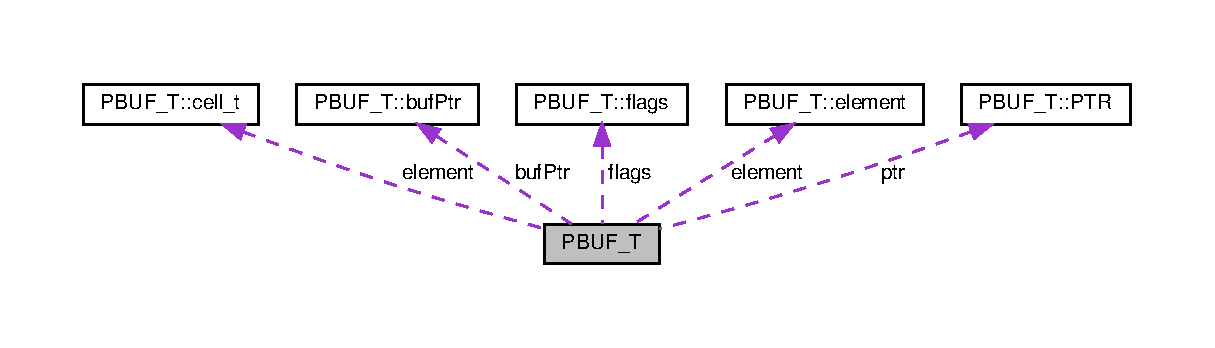
\includegraphics[width=350pt]{structPBUF__T__coll__graph}
\end{center}
\end{figure}
\subsection*{Classes}
\begin{DoxyCompactItemize}
\item 
struct \hyperlink{structPBUF__T_1_1bufPtr}{buf\+Ptr}
\item 
struct \hyperlink{structPBUF__T_1_1cell__t}{cell\+\_\+t}
\item 
struct \hyperlink{structPBUF__T_1_1element}{element}
\item 
struct \hyperlink{structPBUF__T_1_1flags}{flags}
\item 
struct \hyperlink{structPBUF__T_1_1PTR}{P\+TR}
\end{DoxyCompactItemize}
\subsection*{Public Attributes}
\begin{DoxyCompactItemize}
\item 
\mbox{\Hypertarget{structPBUF__T_aef3f97b88f8a21145beaa76799cfcb4b}\label{structPBUF__T_aef3f97b88f8a21145beaa76799cfcb4b}} 
struct \hyperlink{structPBUF__T_1_1flags}{P\+B\+U\+F\+\_\+\+T\+::flags} {\bfseries flags}
\item 
\mbox{\Hypertarget{structPBUF__T_a3b18661739955d1f5e43ef61bd149a4d}\label{structPBUF__T_a3b18661739955d1f5e43ef61bd149a4d}} 
struct \hyperlink{structPBUF__T_1_1bufPtr}{P\+B\+U\+F\+\_\+\+T\+::buf\+Ptr} {\bfseries buf\+Ptr}
\item 
\mbox{\Hypertarget{structPBUF__T_a2b7b4a5242debfa93e5da8e3e7c9ad4b}\label{structPBUF__T_a2b7b4a5242debfa93e5da8e3e7c9ad4b}} 
struct \hyperlink{structPBUF__T_1_1element}{P\+B\+U\+F\+\_\+\+T\+::element} {\bfseries element} \mbox{[}B\+U\+F\+F\+E\+R\+\_\+\+S\+I\+ZE\mbox{]}
\item 
\mbox{\Hypertarget{structPBUF__T_a66bab8f3abac9b03f494a30ec65deea7}\label{structPBUF__T_a66bab8f3abac9b03f494a30ec65deea7}} 
struct \hyperlink{structPBUF__T_1_1PTR}{P\+B\+U\+F\+\_\+\+T\+::\+P\+TR} {\bfseries ptr}
\item 
\mbox{\Hypertarget{structPBUF__T_abc3293776fceb6ddeb3db09a8ce2f2d7}\label{structPBUF__T_abc3293776fceb6ddeb3db09a8ce2f2d7}} 
struct \hyperlink{structPBUF__T_1_1cell__t}{P\+B\+U\+F\+\_\+\+T\+::cell\+\_\+t} {\bfseries element} \mbox{[}B\+U\+F\+F\+E\+R\+\_\+\+S\+I\+ZE\mbox{]}
\item 
\mbox{\Hypertarget{structPBUF__T_aac34deba1ae4ef415285d9e5a6ae27fa}\label{structPBUF__T_aac34deba1ae4ef415285d9e5a6ae27fa}} 
check\+\_\+t {\bfseries activity}
\end{DoxyCompactItemize}


The documentation for this struct was generated from the following files\+:\begin{DoxyCompactItemize}
\item 
src/backup.\+c\item 
src/priority\+\_\+buffer.\+c\end{DoxyCompactItemize}

\hypertarget{structPointerPair}{}\section{Pointer\+Pair Struct Reference}
\label{structPointerPair}\index{Pointer\+Pair@{Pointer\+Pair}}
\subsection*{Public Attributes}
\begin{DoxyCompactItemize}
\item 
\mbox{\Hypertarget{structPointerPair_a2875d2c1a18176e22513cf845e83d85c}\label{structPointerPair_a2875d2c1a18176e22513cf845e83d85c}} 
void $\ast$$\ast$ {\bfseries pointer}
\item 
\mbox{\Hypertarget{structPointerPair_afa4927f6318fe77182704346b634da13}\label{structPointerPair_afa4927f6318fe77182704346b634da13}} 
void $\ast$ {\bfseries old\+\_\+value}
\end{DoxyCompactItemize}


The documentation for this struct was generated from the following file\+:\begin{DoxyCompactItemize}
\item 
test/unity/extras/fixture/src/unity\+\_\+fixture.\+c\end{DoxyCompactItemize}

\hypertarget{structPBUF__T_1_1PTR}{}\section{P\+B\+U\+F\+\_\+T\+:\+:P\+TR Struct Reference}
\label{structPBUF__T_1_1PTR}\index{P\+B\+U\+F\+\_\+\+T\+::\+P\+TR@{P\+B\+U\+F\+\_\+\+T\+::\+P\+TR}}
\subsection*{Public Attributes}
\begin{DoxyCompactItemize}
\item 
\mbox{\Hypertarget{structPBUF__T_1_1PTR_ad30411383d87fea3c1e525e32d765c9c}\label{structPBUF__T_1_1PTR_ad30411383d87fea3c1e525e32d765c9c}} 
index\+\_\+t {\bfseries tail}
\item 
\mbox{\Hypertarget{structPBUF__T_1_1PTR_a8f68df3abc824c389ee598233f4674ba}\label{structPBUF__T_1_1PTR_a8f68df3abc824c389ee598233f4674ba}} 
index\+\_\+t {\bfseries head} \mbox{[}P\+R\+I\+O\+R\+I\+T\+Y\+\_\+\+S\+I\+ZE\mbox{]}
\end{DoxyCompactItemize}


The documentation for this struct was generated from the following file\+:\begin{DoxyCompactItemize}
\item 
src/priority\+\_\+buffer.\+c\end{DoxyCompactItemize}

\hypertarget{structstateMachine__t}{}\section{state\+Machine\+\_\+t Struct Reference}
\label{structstateMachine__t}\index{state\+Machine\+\_\+t@{state\+Machine\+\_\+t}}
\subsection*{Public Attributes}
\begin{DoxyCompactItemize}
\item 
\mbox{\Hypertarget{structstateMachine__t_a9f499c095594429c8e34ae5c27107b5a}\label{structstateMachine__t_a9f499c095594429c8e34ae5c27107b5a}} 
state\+\_\+t {\bfseries state}
\item 
\mbox{\Hypertarget{structstateMachine__t_a7b3ef4521e2f68efbc13bcb9a8e36efb}\label{structstateMachine__t_a7b3ef4521e2f68efbc13bcb9a8e36efb}} 
void($\ast$ {\bfseries func} )(void)
\end{DoxyCompactItemize}


The documentation for this struct was generated from the following file\+:\begin{DoxyCompactItemize}
\item 
src/cli.\+h\end{DoxyCompactItemize}

\hypertarget{structUNITY__FIXTURE__T}{}\section{U\+N\+I\+T\+Y\+\_\+\+F\+I\+X\+T\+U\+R\+E\+\_\+T Struct Reference}
\label{structUNITY__FIXTURE__T}\index{U\+N\+I\+T\+Y\+\_\+\+F\+I\+X\+T\+U\+R\+E\+\_\+T@{U\+N\+I\+T\+Y\+\_\+\+F\+I\+X\+T\+U\+R\+E\+\_\+T}}
\subsection*{Public Attributes}
\begin{DoxyCompactItemize}
\item 
\mbox{\Hypertarget{structUNITY__FIXTURE__T_ae5650e8bb94e0d9c75913a112277e445}\label{structUNITY__FIXTURE__T_ae5650e8bb94e0d9c75913a112277e445}} 
int {\bfseries Verbose}
\item 
\mbox{\Hypertarget{structUNITY__FIXTURE__T_aaa9feba9c4991248a4107098e40813ac}\label{structUNITY__FIXTURE__T_aaa9feba9c4991248a4107098e40813ac}} 
unsigned int {\bfseries Repeat\+Count}
\item 
\mbox{\Hypertarget{structUNITY__FIXTURE__T_a98e6483802e9ba8c55cd10f9eec36cb3}\label{structUNITY__FIXTURE__T_a98e6483802e9ba8c55cd10f9eec36cb3}} 
const char $\ast$ {\bfseries Name\+Filter}
\item 
\mbox{\Hypertarget{structUNITY__FIXTURE__T_a9480a05bc2d571c0fe5f8a7872082af1}\label{structUNITY__FIXTURE__T_a9480a05bc2d571c0fe5f8a7872082af1}} 
const char $\ast$ {\bfseries Group\+Filter}
\end{DoxyCompactItemize}


The documentation for this struct was generated from the following file\+:\begin{DoxyCompactItemize}
\item 
test/unity/extras/fixture/src/unity\+\_\+fixture\+\_\+internals.\+h\end{DoxyCompactItemize}

\hypertarget{structUNITY__STORAGE__T}{}\section{U\+N\+I\+T\+Y\+\_\+\+S\+T\+O\+R\+A\+G\+E\+\_\+T Struct Reference}
\label{structUNITY__STORAGE__T}\index{U\+N\+I\+T\+Y\+\_\+\+S\+T\+O\+R\+A\+G\+E\+\_\+T@{U\+N\+I\+T\+Y\+\_\+\+S\+T\+O\+R\+A\+G\+E\+\_\+T}}
\subsection*{Public Attributes}
\begin{DoxyCompactItemize}
\item 
\mbox{\Hypertarget{structUNITY__STORAGE__T_a69613e2d9945fc1ce5a4848613828a1f}\label{structUNITY__STORAGE__T_a69613e2d9945fc1ce5a4848613828a1f}} 
const char $\ast$ {\bfseries Test\+File}
\item 
\mbox{\Hypertarget{structUNITY__STORAGE__T_a0d7f8bf6c8a95ebe237d411f1fc7e345}\label{structUNITY__STORAGE__T_a0d7f8bf6c8a95ebe237d411f1fc7e345}} 
const char $\ast$ {\bfseries Current\+Test\+Name}
\item 
\mbox{\Hypertarget{structUNITY__STORAGE__T_a21674715adf3d4d1ac7f0c459887cf9d}\label{structUNITY__STORAGE__T_a21674715adf3d4d1ac7f0c459887cf9d}} 
const char $\ast$ {\bfseries Current\+Detail1}
\item 
\mbox{\Hypertarget{structUNITY__STORAGE__T_a9d821447e216e215911e8726aa986eec}\label{structUNITY__STORAGE__T_a9d821447e216e215911e8726aa986eec}} 
const char $\ast$ {\bfseries Current\+Detail2}
\item 
\mbox{\Hypertarget{structUNITY__STORAGE__T_aaae2021491b025aabcc55edb3ca5bedf}\label{structUNITY__STORAGE__T_aaae2021491b025aabcc55edb3ca5bedf}} 
U\+N\+I\+T\+Y\+\_\+\+L\+I\+N\+E\+\_\+\+T\+Y\+PE {\bfseries Current\+Test\+Line\+Number}
\item 
\mbox{\Hypertarget{structUNITY__STORAGE__T_a144a353d362e1c98bdbc963443b268dc}\label{structUNITY__STORAGE__T_a144a353d362e1c98bdbc963443b268dc}} 
U\+N\+I\+T\+Y\+\_\+\+C\+O\+U\+N\+T\+E\+R\+\_\+\+T\+Y\+PE {\bfseries Number\+Of\+Tests}
\item 
\mbox{\Hypertarget{structUNITY__STORAGE__T_a6a5463da7d0010ce4f9d80ff0647c7d4}\label{structUNITY__STORAGE__T_a6a5463da7d0010ce4f9d80ff0647c7d4}} 
U\+N\+I\+T\+Y\+\_\+\+C\+O\+U\+N\+T\+E\+R\+\_\+\+T\+Y\+PE {\bfseries Test\+Failures}
\item 
\mbox{\Hypertarget{structUNITY__STORAGE__T_ab0ea61a39989b54885e805e6a35ff300}\label{structUNITY__STORAGE__T_ab0ea61a39989b54885e805e6a35ff300}} 
U\+N\+I\+T\+Y\+\_\+\+C\+O\+U\+N\+T\+E\+R\+\_\+\+T\+Y\+PE {\bfseries Test\+Ignores}
\item 
\mbox{\Hypertarget{structUNITY__STORAGE__T_a075c6b1282c77d13bf2cc4501283da41}\label{structUNITY__STORAGE__T_a075c6b1282c77d13bf2cc4501283da41}} 
U\+N\+I\+T\+Y\+\_\+\+C\+O\+U\+N\+T\+E\+R\+\_\+\+T\+Y\+PE {\bfseries Current\+Test\+Failed}
\item 
\mbox{\Hypertarget{structUNITY__STORAGE__T_a88913ed616a6eb58f3b45b281b7b1ff4}\label{structUNITY__STORAGE__T_a88913ed616a6eb58f3b45b281b7b1ff4}} 
U\+N\+I\+T\+Y\+\_\+\+C\+O\+U\+N\+T\+E\+R\+\_\+\+T\+Y\+PE {\bfseries Current\+Test\+Ignored}
\item 
\mbox{\Hypertarget{structUNITY__STORAGE__T_a4456e2d39fb2858a0406594a1606d21c}\label{structUNITY__STORAGE__T_a4456e2d39fb2858a0406594a1606d21c}} 
jmp\+\_\+buf {\bfseries Abort\+Frame}
\end{DoxyCompactItemize}


The documentation for this struct was generated from the following file\+:\begin{DoxyCompactItemize}
\item 
test/unity/src/unity\+\_\+internals.\+h\end{DoxyCompactItemize}

\hypertarget{classunity__to__junit_1_1UnityTestSummary}{}\section{unity\+\_\+to\+\_\+junit.\+Unity\+Test\+Summary Class Reference}
\label{classunity__to__junit_1_1UnityTestSummary}\index{unity\+\_\+to\+\_\+junit.\+Unity\+Test\+Summary@{unity\+\_\+to\+\_\+junit.\+Unity\+Test\+Summary}}
\subsection*{Public Member Functions}
\begin{DoxyCompactItemize}
\item 
\mbox{\Hypertarget{classunity__to__junit_1_1UnityTestSummary_a9c7216043b32f182c07f48bd0e43b888}\label{classunity__to__junit_1_1UnityTestSummary_a9c7216043b32f182c07f48bd0e43b888}} 
def {\bfseries \+\_\+\+\_\+init\+\_\+\+\_\+} (self)
\item 
\mbox{\Hypertarget{classunity__to__junit_1_1UnityTestSummary_afdd46a63352b8ab9acaa8f64ec6c3797}\label{classunity__to__junit_1_1UnityTestSummary_afdd46a63352b8ab9acaa8f64ec6c3797}} 
def {\bfseries run} (self)
\item 
\mbox{\Hypertarget{classunity__to__junit_1_1UnityTestSummary_aa7070ab538f01899a2188a62bdca09ee}\label{classunity__to__junit_1_1UnityTestSummary_aa7070ab538f01899a2188a62bdca09ee}} 
def {\bfseries set\+\_\+targets} (self, target\+\_\+array)
\item 
\mbox{\Hypertarget{classunity__to__junit_1_1UnityTestSummary_a1d9761b8e561dc10ce2997b30a497f68}\label{classunity__to__junit_1_1UnityTestSummary_a1d9761b8e561dc10ce2997b30a497f68}} 
def {\bfseries set\+\_\+root\+\_\+path} (self, path)
\end{DoxyCompactItemize}
\subsection*{Static Public Member Functions}
\begin{DoxyCompactItemize}
\item 
\mbox{\Hypertarget{classunity__to__junit_1_1UnityTestSummary_a8af06f2da95b1ebb819e3c83e37f0700}\label{classunity__to__junit_1_1UnityTestSummary_a8af06f2da95b1ebb819e3c83e37f0700}} 
def {\bfseries usage} (err\+\_\+msg=None)
\end{DoxyCompactItemize}
\subsection*{Public Attributes}
\begin{DoxyCompactItemize}
\item 
\mbox{\Hypertarget{classunity__to__junit_1_1UnityTestSummary_af238e0e3f19b3843e37d36980377ed24}\label{classunity__to__junit_1_1UnityTestSummary_af238e0e3f19b3843e37d36980377ed24}} 
{\bfseries report}
\item 
\mbox{\Hypertarget{classunity__to__junit_1_1UnityTestSummary_a8af33e4fc6faed23b2a7035121a855e5}\label{classunity__to__junit_1_1UnityTestSummary_a8af33e4fc6faed23b2a7035121a855e5}} 
{\bfseries total\+\_\+tests}
\item 
\mbox{\Hypertarget{classunity__to__junit_1_1UnityTestSummary_aa81410197141a91aeb663058c0c77fcb}\label{classunity__to__junit_1_1UnityTestSummary_aa81410197141a91aeb663058c0c77fcb}} 
{\bfseries failures}
\item 
\mbox{\Hypertarget{classunity__to__junit_1_1UnityTestSummary_a2098fb414a6325f8caa816b6b7fe2f4d}\label{classunity__to__junit_1_1UnityTestSummary_a2098fb414a6325f8caa816b6b7fe2f4d}} 
{\bfseries ignored}
\item 
\mbox{\Hypertarget{classunity__to__junit_1_1UnityTestSummary_a6d9d8a1b4a93d9ed2b0d9d86408f190c}\label{classunity__to__junit_1_1UnityTestSummary_a6d9d8a1b4a93d9ed2b0d9d86408f190c}} 
{\bfseries targets}
\item 
\mbox{\Hypertarget{classunity__to__junit_1_1UnityTestSummary_a4784068dcc7cfacf63c95bf8bde05a3e}\label{classunity__to__junit_1_1UnityTestSummary_a4784068dcc7cfacf63c95bf8bde05a3e}} 
{\bfseries root}
\item 
\mbox{\Hypertarget{classunity__to__junit_1_1UnityTestSummary_ae73ffcabd682b592454f35c230de4bf1}\label{classunity__to__junit_1_1UnityTestSummary_ae73ffcabd682b592454f35c230de4bf1}} 
{\bfseries test\+\_\+suites}
\end{DoxyCompactItemize}


The documentation for this class was generated from the following file\+:\begin{DoxyCompactItemize}
\item 
test/unity/auto/unity\+\_\+to\+\_\+junit.\+py\end{DoxyCompactItemize}

\hypertarget{classunity__test__summary_1_1UnityTestSummary}{}\section{unity\+\_\+test\+\_\+summary.\+Unity\+Test\+Summary Class Reference}
\label{classunity__test__summary_1_1UnityTestSummary}\index{unity\+\_\+test\+\_\+summary.\+Unity\+Test\+Summary@{unity\+\_\+test\+\_\+summary.\+Unity\+Test\+Summary}}
\subsection*{Public Member Functions}
\begin{DoxyCompactItemize}
\item 
\mbox{\Hypertarget{classunity__test__summary_1_1UnityTestSummary_a7d10482c28be1ca8844eafb7bb2d0516}\label{classunity__test__summary_1_1UnityTestSummary_a7d10482c28be1ca8844eafb7bb2d0516}} 
def {\bfseries \+\_\+\+\_\+init\+\_\+\+\_\+} (self)
\item 
\mbox{\Hypertarget{classunity__test__summary_1_1UnityTestSummary_a191111866f7267d605db2f8793ef9a1a}\label{classunity__test__summary_1_1UnityTestSummary_a191111866f7267d605db2f8793ef9a1a}} 
def {\bfseries run} (self)
\item 
\mbox{\Hypertarget{classunity__test__summary_1_1UnityTestSummary_a5a8af2531586e22b4315e5d09d283cb7}\label{classunity__test__summary_1_1UnityTestSummary_a5a8af2531586e22b4315e5d09d283cb7}} 
def {\bfseries set\+\_\+targets} (self, target\+\_\+array)
\item 
\mbox{\Hypertarget{classunity__test__summary_1_1UnityTestSummary_ae03b008285e29a16d2069120878a2c96}\label{classunity__test__summary_1_1UnityTestSummary_ae03b008285e29a16d2069120878a2c96}} 
def {\bfseries set\+\_\+root\+\_\+path} (self, path)
\item 
\mbox{\Hypertarget{classunity__test__summary_1_1UnityTestSummary_a066f34e5b57d43f0d2397b0e84f5d92b}\label{classunity__test__summary_1_1UnityTestSummary_a066f34e5b57d43f0d2397b0e84f5d92b}} 
def {\bfseries usage} (self, err\+\_\+msg=None)
\item 
\mbox{\Hypertarget{classunity__test__summary_1_1UnityTestSummary_a9baaa8a7f8b862b125f8991c359b2252}\label{classunity__test__summary_1_1UnityTestSummary_a9baaa8a7f8b862b125f8991c359b2252}} 
def {\bfseries get\+\_\+details} (self, result\+\_\+file, lines)
\item 
\mbox{\Hypertarget{classunity__test__summary_1_1UnityTestSummary_ae79303d5a81b382b06c557d6c5bf72e8}\label{classunity__test__summary_1_1UnityTestSummary_ae79303d5a81b382b06c557d6c5bf72e8}} 
def {\bfseries parse\+\_\+test\+\_\+summary} (self, summary)
\end{DoxyCompactItemize}
\subsection*{Public Attributes}
\begin{DoxyCompactItemize}
\item 
\mbox{\Hypertarget{classunity__test__summary_1_1UnityTestSummary_a3e9af40b0081ce3e86ddc63e1fbfa043}\label{classunity__test__summary_1_1UnityTestSummary_a3e9af40b0081ce3e86ddc63e1fbfa043}} 
{\bfseries report}
\item 
\mbox{\Hypertarget{classunity__test__summary_1_1UnityTestSummary_abd63a450624526e498bdc1499078f124}\label{classunity__test__summary_1_1UnityTestSummary_abd63a450624526e498bdc1499078f124}} 
{\bfseries total\+\_\+tests}
\item 
\mbox{\Hypertarget{classunity__test__summary_1_1UnityTestSummary_a67dd44048def2d9bde0385dad9495666}\label{classunity__test__summary_1_1UnityTestSummary_a67dd44048def2d9bde0385dad9495666}} 
{\bfseries failures}
\item 
\mbox{\Hypertarget{classunity__test__summary_1_1UnityTestSummary_a65e84f84c4ebb04f5da3affb20366fe9}\label{classunity__test__summary_1_1UnityTestSummary_a65e84f84c4ebb04f5da3affb20366fe9}} 
{\bfseries ignored}
\item 
\mbox{\Hypertarget{classunity__test__summary_1_1UnityTestSummary_aad532f6e4d7b4af23abd0410aecbfb51}\label{classunity__test__summary_1_1UnityTestSummary_aad532f6e4d7b4af23abd0410aecbfb51}} 
{\bfseries targets}
\item 
\mbox{\Hypertarget{classunity__test__summary_1_1UnityTestSummary_a8cda0aae4f52ce974faace17a99eff79}\label{classunity__test__summary_1_1UnityTestSummary_a8cda0aae4f52ce974faace17a99eff79}} 
{\bfseries root}
\end{DoxyCompactItemize}


The documentation for this class was generated from the following file\+:\begin{DoxyCompactItemize}
\item 
test/unity/auto/unity\+\_\+test\+\_\+summary.\+py\end{DoxyCompactItemize}

%--- End generated contents ---

% Index
\backmatter
\newpage
\phantomsection
\clearemptydoublepage
\addcontentsline{toc}{chapter}{Index}
\printindex

\end{document}
